\documentclass[11pt]{article}
\usepackage[a4paper,margin=18mm]{geometry}
\usepackage[no-math]{fontspec}
\setmainfont{Latin Modern Roman}
\usepackage{amsmath,amssymb,amsthm,xfrac,xspace,hyperref,graphicx,comment}
\excludecomment{DefTralics}
\providecommand{\dpl}{\displaystyle}
\providecommand{\backmatter}{}
\providecommand{\loccit}{\emph{loc. cit.}}

\providecommand{\bibliofont}{\small}
\newcommand{\ie}{i.e.,\xspace}
\newcommand{\eg}{e.g.,\xspace}
\newcommand{\etc}{etc.\xspace}
\newcommand{\cf}{cf.\xspace}
\newcommand{\resp}{resp.\xspace}
\newcommand{\smaller}{\small}
\newcommand{\Subsection}{\subsection}
\newcommand{\Subsubsection}{\subsubsection}
\newcommand{\skpt}{\smallskip}
\emergencystretch=3em
\newfontfamily\jepbibapostrophefont[Path=/usr/share/fonts/truetype/noto/,ItalicFont=NotoSerif-Regular.ttf,BoldFont=NotoSerif-Regular.ttf,BoldItalicFont=NotoSerif-Regular.ttf]{NotoSerif-Regular.ttf}
\catcode`\ʼ=\active
\defʼ{{\jepbibapostrophefont\char"02BC}}

% Begin literal retained input author-preamble.tex
\usepackage[scr=rsfs,cal=euler]{mathalfa}

% Literal retained local macro bbm
\RequirePackage{fontspec}
\newfontfamily\jepbbmonefont[Path=/usr/share/fonts/truetype/noto/,ItalicFont=NotoSansMath-Regular.ttf,BoldFont=NotoSansMath-Regular.ttf,BoldItalicFont=NotoSansMath-Regular.ttf]{NotoSansMath-Regular.ttf}
\DeclareRobustCommand{\mathbbm}[1]{%
\begingroup\def\jepobservedarg{#1}\def\jepallowedarg{1}%
\ifx\jepobservedarg\jepallowedarg
\mathord{\text{\jepbbmonefont\upshape\char"1D7D9}}%
\else\PackageError{bbm}{Unsupported mathbbm argument}{Only the source-observed digit1 is admitted by this scoped renderer.}%
\fi\endgroup}


\multlinegap0pt
\hyphenation{because deformed dimen-sion-al involves sym-met-riza-tion}
\AtBeginDocument{%
\renewcommand{\labelitemi}{$\scriptscriptstyle\bullet$}%
}
\let\epsilon\varepsilon
\newcommand\mto{\mathchoice{\longmapsto}{\mapsto}{\mapsto}{\mapsto}}
\newcommand\hto{\mathrel{\lhook\joinrel\to}}
\newcommand{\onto}{\mathchoice{\to\hspace*{-5mm}\to}{\to\hspace*{-2.85mm}\to}{\to\hspace*{-3mm}\to}{\to\hspace*{-3mm}\to}}

\newcommand{\GL}{\mathrm{GL}}
\newcommand{\SL}{\mathrm{SL}}
\newcommand{\SH}{\mathrm{SH}}
\newcommand{\rU}{\mathrm{U}}


\usepackage{tensor}
\graphicspath{{wen_figures}}

\newtheorem{thm}{Theorem}[section]
\newtheorem*{main}{Main Theorem}
\newtheorem{prop}[thm]{Proposition}
\newtheorem{lem}[thm]{Lemma}
\newtheorem{cor}[thm]{Corollary}

\theoremstyle{definition}
\newtheorem{defn}[thm]{Definition}
\newtheorem{rem}[thm]{Remark}
\newtheorem*{nota}{Notation}

\newcommand{\qqq}{\mathfrak{q}}
\newcommand{\ddd}{\mathfrak{d}}
\newcommand{\QQ}{\mathbb{Q}}
\newcommand{\RR}{\mathbb{R}}
\newcommand{\ZZ}{\mathbb{Z}}
\newcommand{\Hilb}{\mathrm{Hilb}}
\newcommand{\CC}{\mathbb{C}}
\newcommand{\PP}{\mathcal{P}}
\newcommand{\Hom}{\mathrm{Hom}}
\newcommand{\Rep}{\mathrm{Rep}}
\newcommand{\gl}{\mathfrak{gl}}
\newcommand{\hh}{\mathfrak{h}}
\newcommand{\ppp}{\mathfrak{p}}
\newcommand{\VV}{\mathcal{V}}
\newcommand{\NN}{\mathbb{N}}
\newcommand{\OO}{\mathcal{O}}
\newcommand{\UU}{\mathcal{U}}
\newcommand{\DD}{\mathcal{D}}
\newcommand{\WW}{\mathcal{W}}
\newcommand{\AAA}{\mathcal{A}}
\newcommand{\WWo}{\WW^\circ}
\newcommand{\MM}{\mathcal{M}}
\newcommand{\SHH}{\mathcal{S}\ddot{\mathcal{H}}}
\newcommand{\HH}{\ddot{\mathcal{H}}}
\newcommand{\git}{/\kern-.35em/}
\newcommand{\KK}{\mathbb{K}}
\newcommand{\Proj}{\mathrm{Proj}}
\newcommand{\quot}{\mathrm{quot}}
\newcommand{\core}{\mathrm{core}}
\newcommand{\Sym}{\mathrm{Sym}}
\newcommand{\FF}{\mathbb{F}}
\newcommand{\Span}[1]{\mathrm{span}\{#1\}}
\newcommand{\UTor}{\rU_{\qqq,\ddd}(\ddot{\mathfrak{sl}}_\ell)}
\newcommand{\Sss}{\mathcal{S}}
\newcommand{\Hecke}{\mathcal{H}}
\newcommand{\ee}{\boldsymbol{s}}
\newcommand{\xx}{\boldsymbol{x}}
\newcommand{\del}{\partial}
\newcommand{\ad}{\mathrm{ad}}
\newcommand{\tr}{\mathrm{tr}}
\newcommand{\rrr}{\mathfrak{r}}

% End literal retained input author-preamble.tex

\graphicspath{{wen_figures/}}
\begin{document}
\begin{center}{\Large Stable item 2518}\end{center}
\paragraph{Source and attribution.}
Joshua Jeishing Wen, \emph{Quantum Harish-Chandra isomorphism for the double affine Hecke algebra of GL$_n$}, Journal de l’École polytechnique — Mathématiques 13 (2026), publisher version, DOI 10.5802/jep.326. \href{https://jep.centre-mersenne.org/articles/10.5802/jep.326/}{Publisher article}. Authors' text: \href{https://creativecommons.org/licenses/by/4.0/}{CC BY 4.0}.
\paragraph{Editorial problem boundary.}
Prove exactly original Theorem5.20: over $K=\mathbb C(q,t)$ for the printed Jordan quiver and one-dimensional framing, the constructed generic radial-parts map identifies the quantum Hamiltonian reduction with the faithful polynomial-representation image of spherical $\mathrm{GL}_n$ DAHA. Retain the full new quantum-trace/degeneration and Verma restricted-action/moment/Pieri/generic-specialization core. Native2239 prints a self-referential base-change summary,2244 prints $t^{pm 1}$ literally, and2336 prints $\mathfrak{rad}_k$ in the generic inclusion; preserve these alongside the exact1966--1970 setup,2185 coefficient ring,2238 invariant quotient and all four actual $\mathfrak{rad}_\alpha$ generator identities2341--2344. No definition, exponent or subscript is repaired. The generic proof uses arbitrarily large integral $k$ in the common $k>2n$ generator range; the separate printed all-$k>n$ specialization assertion is unselected. The original drawing-exercise label2131 for ribbon-isotopy associativity is retained with the full product/action diagrams, and the unproved action on the entire tHom space2195 is not selected; only the fully authored restricted action is used. No modular-transformation Appendix outcome or arbitrary numerical-parameter specialization is selected. The32 exact source unit/one-dimensional representation glyphs are rendered by a scoped installed Noto Sans Math U+1D7D9 renderer with ordinary mathord spacing, original-size adaptation and unknown-argument rejection; this typography substitution is disclosed. The two U+02BC apostrophes in the original bibliography names use scoped installed Noto Serif punctuation.
\paragraph{Difficulty (editorial): H3.}
The published ribbon-category, Macdonald and PBW prerequisites do not themselves construct the generic radial-parts action because the required Verma modules have no coevaluation. The author supplies new admissible-diagram and restricted-action constructions, verifies the full quantum moment reduction, and proves Pieri preservation and compatibility at infinitely many integral specializations. The remaining generic isomorphism then uses the fully retained local invariant/classical-degeneration dimension and finite-generation/localization arguments, rather than being a formal relabeling of the finite-dimensional theorem.
\paragraph{Editorial transcription note.}
Original author language, mathematics and ordering are preserved. Publisher front matter is replaced by this independent article wrapper. Bibliography is recovered from matching cached publisher HTML, including its TeX formulas. No new proof or mathematical repair is supplied. Surrounding original results are retained for conservative context and are not extra selected corpus claims.
\clearpage

% Begin literal retained input author-body.tex
\section{Introduction}
This paper proves a quantum/multiplicative analogue of the \textit{Harish-Chandra isomorphism}, a result at the source of many fruitful directions of research.
For a complex reductive group $G$ with Lie algebra $\mathfrak{g}$, Cartan subalgebra $\mathfrak{t}$, and Weyl group $W$, the classical isomorphism is concerned with the ring of differential operators $D(\mathfrak{g})$.
Harish-Chandra's \textit{radial parts} map \cite{HCInvDiff} is a homomorphism $D(\mathfrak{g})^G\to D(\mathfrak{t})^W$ that is in some sense a restriction to $\mathfrak{t}$ ``performed with extra steps''.
It was proved to be surjective by Wallach \cite{WallachInv} and Levasseur--Stafford \cite{LevStafJams}, and the latter also determined its kernel \cite{LevStafKer}: the adjoint action induces a homomorphism $\mu:\mathfrak{g}\to D(\mathfrak{g})$ and the kernel is the $G$ invariants of the left ideal $\mathfrak{I}:= D(\mathfrak{g})\mu(\mathfrak{g})$.
Altogether, we~have a description of $D(\mathfrak{t})^W$ as a \textit{quantum Hamiltonian reduction}:
\[
\left[ D(\mathfrak{g})\big/\mathfrak{I} \right]^G\cong D(\mathfrak{t})^W.
\]
The radial parts map is of fundamental importance in the application of rings of differential operators to geometric representation theory (see references cited above).

In the case $G=\GL_n$, this construction admits a 1-parameter deformation, discovered by Etingof--Ginzburg \cite{EtGinz}.
The smash product $D(\mathfrak{h})\rtimes W$ can be deformed via a parameter $c$ to the \textit{rational Cherednik algebra} $H_n(c)$ of the symmetric group~$\Sigma_n$; $D(\mathfrak{h})^W$ is then replaced with the \textit{spherical subalgebra} $\SH_n(c)$.
On the other side, we~consider $D(\mathfrak{gl}_n\times\CC^n)$.
The adjoint and vector representations give a map $\mu:\mathfrak{gl}_n\to D(\mathfrak{gl}_n\times\CC^n)$, and the deformation parameter $c$ appears in the ideal via the trace character $\tr:\mathfrak{gl}_n\to\CC$:
\begin{align*}
\mathfrak{I}_c&:=D(\mathfrak{gl}_n\times\CC^n)\big((\mu-c\tr)(\mathfrak{gl}_n) \big),\\
\mathfrak{A}_c&:= \bigl[ D(\mathfrak{gl}_n\times\CC^n)\big/\mathfrak{I}_c \bigr]^G.
\end{align*}
The \textit{deformed Harish-Chandra isomorphism} was proved by Gan--Ginzburg \cite{GanGinz}:
\begin{equation}
\mathfrak{A}_c\cong \SH_n(c).
\label{DefHC}
\end{equation}
$\mathfrak{A}_c$ is a natural quantization of the Hilbert scheme $n$ points in $\CC^2$, constructed via Hamiltonian reduction as a \textit{Nakajima quiver variety} for the Jordan quiver:
\begin{equation}
\begin{array}{c}
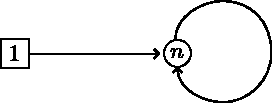
\includegraphics[scale=.8]{../assets/2518/wen_figures/Jordan.pdf}
\end{array}
\label{Jordan}
\end{equation}
Various constructions exist \cite{BFG, GorStaff2, KashRouq} to microlocalize modules for $\mathfrak{A}_c$ into coherent sheaves on the Hilbert scheme, and the isomorphism \eqref{DefHC} allows a rich interplay between such sheaves and representations of $H_n(c)$; in particular, $H_n(c)$ itself microlocalizes to Haiman's \textit{Procesi bundle} \cite{HaimPoly}.

The ladder of deformation affords us more rungs\footnote{Let us that mention that the intermediate step relating differential operators on $\GL_n$ and the \textit{trigonometric} DAHA was done by Finkelberg--Ginzburg \cite{FGCurve}.}---the rational Cherednik algebra is itself a degeneration of the double affine Hecke algebra (DAHA) $\HH_n(q,t)$, an algebra that has appeared across many fields since its initial discovery and application by Cherednik to solving conjectures from the theory of Macdonald polynomials \cite{ChereAnnals}.
It is natural to ask if there is an analogue of the Harish-Chandra isomorphism for $\HH_n(q,t)$ and, more specifically, its spherical subalgebra $\SHH_n(q,t)$.
One can view the ring $D(\mathfrak{gl}_n)$ as $\CC[\mathfrak{gl}_n]\otimes\CC[\mathfrak{gl}_n]$ with a nontrivial commutation relation between the two tensorands.
It is almost immediately obvious that $D(\mathfrak{gl}_n)$ would need to be replaced by an algebra quantizing $\CC[\GL_n]\otimes\CC[\GL_n]$; this is no longer the coordinate ring of a cotangent bundle and thus there is no quantization via differential operators that is available to us ``out of the box''.
Moreover, to perform quantum Hamiltonian reduction, the algebra structure of the quantization needs to be equivariant with respect to whatever symmetry object replaces $\GL_n$.

The correct quantization was defined by Varagnolo--Vasserot \cite{VarVassRoot}: this is their ring of \textit{quantum differential operators} on $\GL_n$, which we denote by $\DD$.
Here, $\GL_n$-equivariance is replaced with equivariance with respect to the quantized universal enveloping algebra $\UU:=\rU_q(\mathfrak{gl}_n)$.
As a $\UU$-module, $\DD$ is isomorphic to the tensor product of two copies of $\OO:=\OO_q(\GL_n)$, an equivariant version of functions on quantum $\GL_n$.
One can construct $\OO$ from the braided monoidal category of finite-dimensional $\UU$-modules via a braided analogue of Tannakian reconstruction discovered by Majid \cite{MajidBraided}, and it is also a localization of what is called the \textit{reflection equation algebra} \cite{DonMudRET}.
$\DD$ also appeared in prior work of Alekseev--Schomerus \cite{AlekScho} on quantizations of character varieties.

Varagnolo--Vasserot also address the other necessary ingredients, but we follow the definitions of Jordan in his construction of \textit{quantized multiplicative quiver varieties} \cite{JordanMult}.
Out of the same quiver data \eqref{Jordan}, this yields a $\CC(q,t)$-algebra $\mathcal{A}_t$ through a Hopf-algebraic version of quantum Hamiltonian reduction.
Our main result is the following:

\begin{main}
The quantized multiplicative quiver variety $\mathcal{A}_t$ for the quiver data~\eqref{Jordan} is isomorphic as a $\CC(q,t)$-algebra to the spherical $\GL_n$-DAHA $\SHH_n(q,t)$.
\end{main}

Thus, the two algebras are isomorphic for generic values of the parameters~$q$ and~$t$.
Prior to our result, the analogous isomorphism was proved in the following cases:
\begin{itemize}
\item when $q=1$ \cite{ObDAHA};
\item when $q$ is a root of unity of sufficiently large order \cite{VarVassRoot};
\item formally over the ring $\CC[\![\hbar]\!]$ where $q=e^\hbar$ \cite{JordanMult};
\item for any $q\in\CC^\times$ and $n=2$ \cite{BalJor}.
\end{itemize}

Our strategy follows the well-established pattern from the rational case \cite{GanGinz, EGGO}.
Both sides of the isomorphism are invariant subalgebras, and thus one does not have a presentation for either; from a general perspective, one may be curious about techniques for proving two algebras are isomorphic without generators and relations.
In the rational case, the scheme of proof goes as follows:
\begin{enumerate}
\item\label{enum:1} embed $\SH_n(c)$ into a ring of differential operators via a \textit{Dunkl representation};
\item\label{enum:2} map $\mathfrak{A}_c$ to that same ring via a deformed analogue of the Harish-Chandra radial parts map;
\item\label{enum:3} show that the radial parts map is injective and surjects onto the image of $\SH_n(c)$.
\end{enumerate}
$\SHH_n(q,t)$ has an analogue of \eqref{enum:1}, the \textit{Dunkl-Cherednik} embedding into a ring of difference operators.
Step \eqref{enum:2} is not straightforward, but Varagnolo--Vasserot \cite{VarVassRoot} gave a brilliant definition for a \textit{quantum radial parts map}.
Namely, the equivariance of $\mathcal{A}_t$ ensures that it acts on certain spaces of intertwiners, and Etingof--Kirillov have identified the weighted traces of these intertwiners with Macdonald polynomials \cite{EtKirQuant}. We~perform step \eqref{enum:3} first for the case $t=q^k$, wherein we use work of Jordan \cite{JordanMult} to perform a classical degeneration $q\mto 1$.

Finally, leveraging the $t=q^k$ case to general $t$ requires some care because the Etingof--Kirillov construction for general $t$ uses Verma modules.
Our approach to step~\eqref{enum:2} at $t=q^k$ involves the diagrammatic calculus afforded by the ribbon category structure of the category of finite-dimensional $\UU$-modules.
Much of this structure persists for Verma modules because they are highest weight; however, being infinite-dimensional, they lack a coevaluation map.
This prevents a straightforward application of our approach to the radial parts map to the case of general $t$.
Nonetheless, in~\ref{GenPar}, we~define a diagrammatic action of $\mathcal{A}_t$ on Etingof--Kirillov intertwiners for general~$t$ by turning part of the diagrams upside-down.
This construction of the radial parts map for generic parameters specializes compatibly to the $t=q^k$ case, and step~\eqref{enum:3} follows essentially from Nakayama's Lemma.

\subsubsection*{Further directions}
While it is unclear to us if a geometric story as in the rational case can be repeated here, the multiplicative setting is interesting due to its relation to character varieties for the torus.
In \cite{AlekScho} as well as the more recent \cite{BBJ1,BBJ2}, $\AAA_t$ has been realized as a quantized character variety. We~have added an appendix that tracks down how the $\SL_2(\ZZ)$-action of the DAHA is manifested in $\AAA_t$, which may be interesting from a topological perspective.
Let us note the similarities to conjectures of Morton--Samuelson \cite{MortSamDAHA} concerning DAHAs and skeins (proved in \cite{BCMN}).

Shortly after the initial posting of this paper, we~received the extremely interesting work \cite{GJV}, which initiates a quantum analogue of Springer theory through the beautiful idea of $q$-deforming the Hotta--Kashiwara $D$-module \cite{HottKash}.
In type $A$, the authors are indeed able to relate their construction to Weyl group representations.
Critical to this result is the isomorphism between $\AAA_q$ and a spherical DAHA via Jordan's \textit{elliptic Schur--Weyl duality} \cite{JordanEll,JorVaz}, which is only available in type $A$.
On the other hand, we~can also obtain such an isomorphism via the radial parts map at $t=q$, wherein both algebras act on characters.
This approach generalizes to other types, although significant challenges remain in establishing such an isomorphism.

\section{Double affine Hecke algebras}

In this section, we~review the $\GL_n$ DAHA and associated structures.
Our main reference is \cite{ChereDAHA}, although in order to make better contact with Etingof--Kirillov theory, we~follow the conventions from \cite{KirLec}.

\subsection{Definition}
Let $R:=\CC[q^{\pm1},t^{\pm1}]$ and $K:=\CC(q,t)$.
The $\GL_n$-DAHA $\HH_n(q,t)$ is the $K$-algebra with generators
\[
\{T_i,
X_j^{\pm 1},
\pi^{\pm 1}\, |\,i=1,\ldots, n-1\hbox{ and } j=1,\ldots, n\}
\]
and relations
\begin{equation*}
\begin{aligned}
&(T_i-t)(T_i+t^{-1})=0;&&X_iX_j=X_jX_i; \\
&T_iT_{i+1}T_i=T_{i+1}T_iT_{i+1};&& T_iT_j=T_jT_i\hbox{ for }j\not=i, i+1;\\
&T_iX_j=X_jT_i\hbox{ for }j\not=i, i+1; && T_iX_iT_i=X_{i+1}; \\
&\pi T_i=T_{i+1}\pi; && \pi^n T_i=T_i\pi^n;\\
&\pi X_i=X_{i+1}\pi;&& \pi X_n=q^{-2}X_1\pi.
\end{aligned}
\end{equation*}
We can also define this as an $R$-algebra, which we denote by $\HH^R_n(q,t)$.

\subsubsection{Y-generators}\label{YGen}
The elements
\begin{equation}
Y_i:= T_i\cdots T_{n-1}\pi^{-1} T_1^{-1}\cdots T_{i-1}^{-1}
\label{YDef}
\end{equation}
for $i=1,\ldots,n$ generate a polynomial subalgebra.
They furnish an alternative presentation of $\HH_n(q,t)$, now with generators
\[
\left\{ T_i, X_j^{\pm 1}, Y_j^{\pm 1} \, | \, i=1,\ldots, n-1\hbox{ and }j=1,\ldots, n\right\}
\]
and relations
\begin{equation}
\begin{aligned}
&(T_i-t)(T_i+t^{-1})=0;\\
&T_iT_{i+1}T_i=T_{i+1}T_iT_{i+1};&& T_iT_j=T_jT_i\hbox{ for }j\not=i, i+1;\\
&X_iX_j=X_jX_i; && Y_iY_j=Y_jY_i;\\
&T_i X_i T_i=X_{i+1}\hbox{ for }i\not=n; && T_i^{-1}Y_iT_i^{-1}=Y_{i+1}\hbox{ for }i\not=n;\\
&T_iX_j=X_jT_i\hbox{ for }j\not=i, i+1;&&T_iY_j=Y_jT_i\hbox{ for }j\not=i, i+1;\\
&Y_1\cdots Y_nX_j=q^2X_jY_1\cdots Y_n;&& X_1\cdots X_nY_j=q^{-2}Y_jX_1\cdots X_n;\\
&X_1Y_2=Y_2T^2_1X_1.
\end{aligned}
\label{DAHAY}
\end{equation}
We note that this presentation is also valid for $\HH_n^R(q,t)$.
From these relations, we~can define a bigrading on $\HH_n^R(q,t)$ by setting:
\[
\deg(X_j^{\pm 1})= (\pm 1,0),\quad
\deg(Y_j^{\pm 1})= (0,\pm 1),\quad
\deg(T_i)= (0,0).
\]

\subsubsection{Symmetrizer}\label{Symmetrizer}
The subalgebra $\Hecke_n(t)$ of $\HH_n(q,t)$ generated by $T_1,\ldots, T_{n-1}$ is isomorphic to the usual Hecke algebra for the symmetric group $\Sigma_n$ with parameter~$t$.
As such, one can make sense of elements $T_w\in\Hecke_n(t)$ for any $w\in \Sigma_n$.
Specifically, first let $s_{i}\in\Sigma_n$ be the $i$th adjacent transposition.
For any reduced expression $w=s_{i_1}\cdots s_{i_a}$, the element
\[
T_w:=T_{i_1}\cdots T_{i_a}
\]
is independent of the reduced expression.
Letting $\ell(w)=a$ denote the length, define the symmetrizer
\[
\tilde{\ee}:=\sum_{w\in\Sigma_n}t^{\ell(w)}T_w.
\]
It will be useful to note the following:
\begin{align}
T_i\tilde{\ee}=\tilde{\ee} T_i&= t\tilde{\ee}\quad\text{for all $i$,}\label{EAbsorb}\\
\sum_{w\in \Sigma_n}s^{\ell(w)}&=[n]_s!,\nonumber\\[
-3pt]
\tilde{\ee}^2&=[n]_{t^2}!\tilde{\ee},\label{EIdem}
\end{align}
where
\[
[\pm k]_s=\frac{1-s^{\pm k}}{1-s^{\pm 1}},\quad [k]_s!=[k]_s[k-1]_s\cdots [1]_s
\]
for $k\in\NN$.
From \eqref{EIdem},
\[
\ee:=\frac{\tilde{\ee}}{[n]_{t^2}!}
\]
is an idempotent.

\subsubsection{Triangular decomposition}
For a vector $v=(v_1,\ldots, v_n)\in\ZZ^n$, denote the monomial
\[
Y^{v}:=Y_1^{v_1}\cdots Y_n^{v_n}.
\]
The following is \cite[Th.\,2.3(ii)]{ChereAnnals}:
\begin{thm}
Any $H\in\HH_n^R(q,t)$ can be uniquely written as
\begin{equation}
H=\sum_{\substack{w\in\Sigma_n\\ v\in\ZZ^n}}Y^vf_{v,w}(X^{\pm 1}_1,\ldots,X^{\pm 1}_n)T_w
\label{DAHAPBW}
\end{equation}
for some Laurent polynomials $\{f_{v,w}\}$ with coefficients in $R$.
\end{thm}

\begin{cor}\label{DAHAFree}
$\HH_n^R(q,t)$ is a free $R$-module.
\end{cor}

\subsection{Spherical DAHA}
The \textit{spherical subalgebra} $\SHH_n(q,t)$ is defined as
\[
\SHH_n(q,t):=\ee\HH_n(q,t)\ee\subset\HH_n(q,t).
\]
We denote the localizations $\tilde{R}:=R[(1-t^{2k})^{-1}]_{k>0}$ and $\HH^{\tilde{R}}_n(q,t):=\tilde{R}\otimes \HH^R_n(q,t)$.
Note that $\ee\in \HH^{\tilde{R}}_n(q,t)$, and we define
\[
\SHH_n^R(q,t):=\ee\HH_n^{\tilde{R}}(q,t)\ee.
\]
We then make sense of the specialization $t=q^k$ by setting
\begin{align*}
\SHH_n^R(q,q^k)&:=\SHH_n^R(q,t)\big|_{t=q^k},\\
\SHH(q,q^k)&:=\CC(q)\otimes\SHH_n^R(q,q^k).
\end{align*}

\subsubsection{Bigrading revisited}\label{DAHABigrad}
Multiplying both sides of \eqref{DAHAPBW} by $\ee$ and absorbing the~$T_w$ into $\ee$ using \eqref{EAbsorb}, we~can see that $\SHH_n^R(q,t)$ is spanned by elements of the~form
\[
\ee \Bigl(\sum_{v\in\ZZ^n}Y^vf(X_1^{\pm 1},\ldots, X_n^{\pm 1})\Bigr)\ee.
\]
For such an element as above that is homogeneous with respect to the bigrading, we~can see from \eqref{DAHAY} that its bidegree can be discerned by commuting with
\begin{equation}
\begin{aligned}
\ee\boldsymbol{X}_n^{\pm1}\ee&:=\ee X_1^{\pm 1}\cdots X_n^{\pm 1}\ee,\\
\hbox{ and }\ee\boldsymbol{Y}_n^{\pm 1}\ee&:=\ee Y_1^{\pm 1}\cdots Y_n^{\pm 1}\ee.
\end{aligned}
\label{DAHADet}
\end{equation}
\begin{prop}
$H\in\SHH_n^R(q,t)$ has bidegree $(a,b)$ if and only if
\begin{align*}
\left(\ee \boldsymbol{X}_n\ee\right) H \left(\ee \boldsymbol{X}_n^{-1}\ee\right)&= q^{-2a}H,&
\left(\ee \boldsymbol{Y}_n\ee\right) H \left(\ee \boldsymbol{Y}_n^{-1}\ee\right)&= q^{2b}H.
\end{align*}
\end{prop}

Let $\HH_n^R(q,t)_{\textrm{IV}}\subset\HH_n^R(q,t)$ denote the subalgebra generated by
\[
\{T_i, X_j, Y^{-1}_j\, |\, i=1,\ldots, n-1\hbox{ and }j=1,\ldots, n\},
\]
\ie we restrict to positive powers of $X$-generators and negative powers of $Y$-generators (the ``fourth quadrant'' in the bigrading). We~then set
\[
\SHH_n^R(q,t)_{\textrm{IV}}:=\ee\bigl(\HH_n^R(q,t)_{\textrm{IV}}\bigr)\ee\subset\SHH_n^R(q,t).
\]
The subalgebras $\SHH_n(q,t)_{\mathrm{IV}}$, $\SHH_n^R(q,q^k)_{\mathrm{IV}}$, and $\SHH_n(q,q^k)_{\mathrm{IV}}$ are defined similarly.
Let $\mathcal{S}^R_{\mathrm{IV}}[a,b]$ denote the homogeneous piece of $\SHH_n^R(q,t)_{\mathrm{IV}}$ of bidegree $(a,b)$ and likewise for
\[
\mathcal{S}_{t,\mathrm{IV}}[a,b]\subset\SHH_n(q,t)_{\mathrm{IV}},\quad
\mathcal{S}_{q^k,\mathrm{IV}}[a,b]\subset\SHH_n(q,q^k)_{\mathrm{IV}}.
\]

Finally, let
\[
\CC[\boldsymbol{x}_n,\boldsymbol{y}_n]:=\CC[x_1,\ldots, x_n, y_1,\ldots, y_n].
\]
The symmetric group $\Sigma_n$ acts on $\CC[\boldsymbol{x}_n,\boldsymbol{y}_n]$ by permuting subscripts.
$\CC[\boldsymbol{x}_n,\boldsymbol{y}_n]$ is also bigraded, where $\deg(x_i)=(1,0)$ and $\deg(y_i)=(0,1)$.
Denote by $\CC[\boldsymbol{x}_n,\boldsymbol{y}_n]^{\Sigma_n}_{a,b}$ the subspace of invariant homogeneous elements of bidegree $(a,b)$.

\begin{prop}\label{IVRank}
We have
\[
\dim_{K}\mathcal{S}_{t,\mathrm{IV}}[a,-b]=\dim_{\CC(q)}\mathcal{S}_{q^k,\mathrm{IV}}[a,-b]=\dim_\CC \CC[\boldsymbol{x}_n,\boldsymbol{y}_n]^{\Sigma_n}_{a,b}.
\]
\end{prop}

\begin{proof}
$\mathcal{S}^R_{\mathrm{IV}}[a,b]$ is a direct summand of the free $R$-module $\HH_n^R(q,t)_{\mathrm{IV}}$ (Corollary~\ref{DAHAFree}).
Therefore, it is also free, and the dimensions of $\mathcal{S}_{t,\mathrm{IV}}[a,b]$ and $\mathcal{S}_{q^k,\mathrm{IV}}[a,b]$ are both equal to its rank.
To compute this rank, we~can set $q=t=1$, in~which case
\[
\HH_n^R(q,t)_{\mathrm{IV}}\big|_{q=t=1}\cong \CC[\boldsymbol{x}_n, \boldsymbol{y}_n]\rtimes\CC[\Sigma_n],\quad
\SHH_n^R(q,t)_{\mathrm{IV}}\big|_{q=t=1}\cong \CC[\boldsymbol{x}_n, \boldsymbol{y}_n]^{\Sigma_n},
\]
where $x_i$ and $y_i$ are the images of $X_i$ and $Y_i^{-1}$, respectively.
\end{proof}

\subsubsection{Generators}\label{Gen}
We use ideas from the proofs of \cite[Prop.\,2.5]{SchiffVassMac} and \cite[Lem.\,5.2]{FFJMM} to produce nice generating sets.
For $r=1,\ldots, n$, Let $e_r$ denote the $r$th elementary symmetric polynomial in $n$ variables and set
\begin{equation}
\begin{aligned}
e_r(\boldsymbol{X}_n^{\pm 1})&:=e_r(X_1^{\pm 1},\ldots, X_n^{\pm 1}),\\
e_r(\boldsymbol{Y}_n^{\pm 1})&:=e_r(Y_1^{\pm 1},\ldots, Y_n^{\pm 1}).
\end{aligned}
\label{ElemXY}
\end{equation}
\begin{lem}[{\cite[Lem.\,A.15.2]{VarVassRoot}}]\label{GenLem}
We have the following:
\begin{enumerate}
\item\label{GenLem1} $\SHH_n(q,t)_{\mathrm{IV}}$ is generated by
\begin{equation}
\left\{ \boldsymbol{s} e_r(\boldsymbol{X}_n)\boldsymbol{s},\boldsymbol{s} e_r(\boldsymbol{Y}_n^{-1})\boldsymbol{s}\, \middle|\, r=1,\ldots, n \right\}
\label{IVGen}
\end{equation}
and $\SHH_n(q,t)$ is generated by the set \eqref{IVGen} along with $\ee \boldsymbol{X}_n^{-1}\ee$ and $\ee \boldsymbol{Y}_n\ee$.
\item\label{GenLem2} The analogous statement holds for $\SHH_n(q,q^k)_{\mathrm{IV}}$ and $\SHH_n(q,q^k)$ for $k>2n$.
\end{enumerate}
\end{lem}

\begin{proof}
For $(a,b)\in\ZZ_{\ge 0}^2$, let
\[
P_{a,-b}=\ee\Bigl(\sum_{i=1}^nX_i^aY_i^{-b}\Bigr)\ee.
\]
First note that by a classical theorem of Weyl \cite{WeylInv}, the invariant polynomial ring $\CC[\boldsymbol{x}_n,\boldsymbol{y}_n]^{\Sigma_n}$ is generated by power sums of the form:
\[
p_{a,b}:=\sum_{i=1}^n x_i^ay_i^{b}=P_{a,-b}\big|_{q=t=1}.
\]
Moreover, by the identity
\[
p_{a,b}=\sum_{i=1}^n(-1)^{i-1}e_i(x_1,\ldots, x_n)p_{a-i,b},
\]
the $p_{a,b}$ with $0\le a\le n$ generate $\CC[\boldsymbol{x}_n,\boldsymbol{y})_n]^{\Sigma_n}$.
Thus, the $P_{a,b}$ with $0\le a\le n$ generate $\SHH_n^R(q,t)_{\mathrm{IV}}$ modulo the ideal $(q-1, t-1)$.
By applying Nakayama's lemma to each (finite rank) bigraded piece, we~get that they generate $\SHH_n(q,t)$ and $\SHH_n(q,q^k)$.

Next, note that $P_{1,0}=\ee e_1(\boldsymbol{X}_n)\ee$ and $P_{0,-1}=\ee e_1(\boldsymbol{Y}_n^{-1})\ee$.
By \eqref{YDef}, $Y_i$ becomes the $q^2$-shift operator on $X_i$ at $t=1$. We~thus have
\begin{align}
\nonumber
\ad\left(P_{1,0} \right)^a\cdot P_{0,-1}&= (1-q^{-2})^aP_{a, -1},\\
\ad\left(P_{0,-1} \right)^b \cdot P_{a, -1}&= (q^{-2a}-1)^bP_{a, -1-b},
\label{PGen}
\end{align}
where $\ad\left(X \right)$ is the adjoint operator:
\[
\ad\left(X \right)=[X,-].
\]
In the case of $\SHH_n(q,t)$, we~have that after localizing to $\CC(q)[t^{\pm 1}]$, any $P_{a,-b}$ with $a,b>0$ can be written in terms of $\ee e_1(\boldsymbol{X}_n)\ee$ and $\ee e_1(\boldsymbol{Y}_n^{-1})\ee$ modulo the ideal $(t-1)$. We~include the other elementary symmetric polynomials to cover the cases $a$ or $b=0$.
The result follows by again apply Nakayama's Lemma to each bigraded piece.
For $\SHH_n(q,q^k)$, we~need to specialize $q=e^{2\pi i/k}$ in order to have $t=1$.
Equation \eqref{PGen} becomes problematic once $a\ge 2k$, but we obtain all $0\le a\le n$ once $k> 2n$.
\end{proof}

\subsection{Polynomial representation}\label{PolRep}
While Lemma \ref{GenLem} gives generators for $\SHH_n(q,t)$ and $\SHH_n(q,q^k)$, we~do not have relations; in compensation, we~have instead a faithful representation.

\subsubsection{Demazure-Lusztig operators}
Let $K[\xx_n^\pm]:=K[x_1^{\pm 1},\ldots x_{n}^{\pm 1}]$ be the ring of Laurent polynomials in $n$ variables. We~similarly use the abbreviation $R[\xx_n^\pm]$.
The symmetric group $\Sigma_n$ acts on both rings by permuting variables, and as before, we~let $s_i\in\Sigma_n$ denote the usual adjacent transposition.

\begin{thm}[{\cite[Th.\,2.3]{ChereAnnals}}]
The following defines a faithful representation $\mathfrak{r}$ of $\HH_{n}^R(q,t)$ on $R[\xx_n^\pm]$: for $f\in K[\xx_n^\pm]$,
\begin{align*}
\mathfrak{r}(T_i)&=ts_i+(t-t^{-1})\frac{s_i-1}{x_i/x_{i+1}-1},\\
\rrr(X_i)f&=x_if,\\
\rrr(\pi)f(x_1,x_2,\ldots, x_n)&=f(x_2,x_3,\ldots, x_n, q^{-2}x_1).
\end{align*}
This representation remains faithful on any specialization of $(q,t)$ so long as $q$ is not sent to a root of unity.
\end{thm}

We will abuse notation and use $\rrr$ to also denote its versions obtained via base-change from $R$.
From the formula for $\rrr(T_i)$, we~can see that
\[
f\in K[\xx_n^\pm]^{\Sigma_n}\hbox{ if and only if }\rrr(T_i)f=tf
\]
for all $i$.
It follows from \eqref{EAbsorb} that the restriction of $\rrr$ to $\SHH_{n}(q,t)$ and $\SHH_n^R(q,t)$ preserves the subring $\Lambda_n^\pm(q,t):=K[\xx_n^\pm]^{\Sigma_n}$. We~similarly define $\Lambda_n^\pm(q)$ in the obvious~way.

The following is well known:
\begin{prop}\label{MacGen}
The elements $\ee e_r(\boldsymbol{X}_n^{\pm 1})\ee$ and $\ee e_r(\boldsymbol{Y}_n^{\pm 1})\ee$ act on $f\in\Lambda^\pm_n(q,t)$ by:
\begin{align*}
\rrr\left(\ee e_r(\boldsymbol{X}_n^{\pm 1})\ee\right) f&=e_r(x_1^{\pm 1},\ldots, x_n^{\pm 1})f,\\
\rrr\left(\ee e_r(\boldsymbol{Y}_n^{\pm 1})\ee\right) f&=\sum_{I\subset\{1,\ldots, n\}}\biggl(\prod_{\substack{i\in I\\ j\not\in I}}\frac{t^2\left(\sfrac{x_i}{x_j}\right)^{\pm 1}-1}{\left(\sfrac{x_i}{x_j}\right)^{\pm 1}-1}\biggr)\prod_{i\in I}T_{q^2, x_i}^{\pm 1} f,
\end{align*}
where $T_{q^2, x_i}f(x_1,\ldots, x_i,\ldots,x_n)=f(x_1,\ldots, q^2x_i,\ldots, x_n)$.
\end{prop}

\subsubsection{Macdonald polynomials}
We will need a nice basis for the representation of $\SHH_n(q,t)$ on $\Lambda^\pm_n(q,t)$.
A natural starting point is the basis of \textit{monomial symmetric functions}: for $\lambda=(\lambda_1,\ldots, \lambda_n)\in\ZZ^n$,
\[
m_\lambda:=\sum_{w\in\Sigma_n/\mathrm{Stab}(\lambda)}x^{w\lambda},
\]
where $\Sigma_n$ acts on $\ZZ^n$ by permutations and for $\mu=(\mu_1,\ldots, \mu_n)\in\ZZ^n$,
\[
x^\mu=x_1^{\mu_1}x_2^{\mu_2}\cdots x_n^{\mu_n}.
\]
We say that $\lambda\in\ZZ^n$ is \textit{dominant} if $\lambda_1\ge\lambda_2\ge\cdots\ge\lambda_n$; it is easy to see that the $m_\lambda$ for dominant $\lambda$ provide a basis of $\Lambda_n^\pm(q,t)$.
\begin{thm}\label{MacThm}
We have the following:
\begin{enumerate}
\item\label{MacThm1} For each dominant $\lambda$, there exists a unique $P_\lambda(q,t)\in\Lambda_n^\pm(q,t)$ satisfying
\begin{itemize}
\item for $f\in\Lambda_n^\pm(q,t)$,
\[
\rrr\left(\ee f(Y_1,\ldots, Y_n)\ee \right)P_\lambda(q,t)=f\left(q^{2\lambda_1}t^{n-1},q^{2\lambda_2}t^{n-3},\ldots,q^{2\lambda_n}t^{1-n}\right)P_\lambda(q,t);
\]
\item the coefficient of $m_\lambda$ is $1$.
\end{itemize}
Moreover, $\left\{ P_\lambda(q,t) \right\}$ form a basis of $\Lambda_n^\pm(q,t)$.
\item\label{MacThm2} For any integer $k>0$, $P_\lambda(q,t)$ can be specialized to $t=q^k$.
\end{enumerate}
\end{thm}

\begin{proof}
Part \eqref{MacThm1} is classical.
For \eqref{MacThm2}, one can consider the \textit{tableaux sum formula} for $P_\lambda(q,t)$ (\cf \cite[VI.6]{MacBook}).
\end{proof}

$P_\lambda(q,t)$ is the \textit{Macdonald polynomial} associated to $\lambda$.

\begin{rem}
When $\lambda$ is a partition (i.e., $\lambda_n\ge 0$), our $P_\lambda(q,t)$ is actually the $P_\lambda(q^2,t^2)$ found in \cite{MacBook}.
As stated in the start of this section, we~make this choice to better align with the Etingof-Kirillov approach to Macdonald polynomials.
\end{rem}

\section{Quantum groups}

\subsection{Quantum enveloping algebra}
In this subsection, we~review the algebra
\[
\mathcal{U}:=\rU_q(\gl_n)
\]
and some of its basic structures.

\subsubsection{Roots and weights}
Let $\epsilon_i\in \RR^n$ be the $i$th coordinate vector.
The \textit{root system}~$R$ is the set $\left\{ \epsilon_i-\epsilon_j \right\}$, and the set of \textit{positive roots} $R^+$ is the subset where $i<j$.
Within~$R^+$, we~call the $n-1$ elements
\[
\alpha_i=\epsilon_i-\epsilon_{i+1}\quad\text{for }i=1,\ldots, n-1
\]
the \textit{simple roots}.
The \textit{root lattice} $Q$ is the lattice spanned by $R$, and we denote by~$Q^+$ the semigroup generated by $R^+$. We~equip $\RR^n$ with the usual symmetric pairing $\langle-,-\rangle$ for which $\left\{ \epsilon_i \right\}$ is an orthonormal basis.

The set of \textit{weights} is the subset
\[
\bigl\{ \omega\in\RR^n\, |\, \langle\omega,\alpha\rangle\in\ZZ\hbox{ for all }\alpha\in R \bigr\}.
\]
For $i=1,\ldots, n$, we~let
\[
\omega_i:=\epsilon_1+\epsilon_2+\cdots+\epsilon_i
\]
denote the \textit{$i$th fundamental weight}.
The lattice spanned by $\left\{ \omega_i \right\}$ is called the \textit{weight lattice} $P$, which is equal to the lattice spanned by $\left\{ \epsilon_i \right\}$.
For $\lambda, \mu\in P$, we~order $\lambda\ge\mu$ if $\lambda-\mu\in Q^+$.
A weight is \textit{dominant} if it pairs non-negatively with all roots.
Let $P^+\subset P$ denote the subset of dominant elements.
This is \textit{not} the set of dominant weights but rather the subset of dominant weights whose coefficient for $\omega_n$ is an integer.
Finally, we~set
\begin{align*}
\rho&:=\Bigl(\frac{n-1}{2}, \frac{n-3}{2},\ldots,\frac{1-n}{2} \Bigr),\\
\delta&:=(n-1, n-2,\ldots, 0).
\end{align*}
Both satisfy $\langle\rho, \alpha_i\rangle =\langle\delta,\alpha_i\rangle=1$ for all $i$ and $\langle\rho,\omega_n\rangle=\langle \delta,\omega_n\rangle=0$.
Note that $2\rho\in P$ but $\rho\not\in P$ if $n$ is even.

\subsubsection{Definition}
$\mathcal{U}$ is the $\CC(q)$-algebra with generators
\[
\left\{ E_i, F_i, q^h\, |\, i=1,\ldots, n-1\hbox{ and }h\in P \right\}
\]
and relations
\begin{gather*}
q^{\vec{0}}=1,\,q^{h_1}q^{h_2}=q^{h_1+h_2},\\
q^hE_iq^{-h}=q^{\langle\alpha_i,h\rangle}E_i,\,q^hF_iq^{-h}=q^{-\langle\alpha_i,h\rangle}F_i,\\
E_iF_j-F_jE_i=\delta_{ij}\dfrac{q^{\alpha_i}-q^{-\alpha_i}}{q-q^{-1}},\\
E_i^2E_{i+1}-(q+q^{-1})E_iE_{i+1}E_i+E_iE_{i+1}^2=0,\\
F_i^2F_{i+1}-(q+q^{-1})F_iF_{i+1}F_i+F_iF_{i+1}^2=0,
\end{gather*}
where $\delta_{ij}$ is the Kronecker delta. We~can endow it with a Hopf algebra structure where the coproduct $\Delta$, counit $\epsilon$, and antipode $S$ are given by
\begin{gather*}
\Delta(E_i)=E_i\otimes q^{\alpha_i}+1\otimes E_i,\hspace{.5cm}\Delta(F_i)=F_i\otimes 1+q^{-\alpha_i}\otimes F_i,\hspace{.5cm}\Delta(q^h)=q^h\otimes q^h;\\
\epsilon(E_i)=\epsilon(F_i)=0,\hspace{.5cm}\epsilon(q^h)=1;\\
S(E_i)=-E_iq^{-\alpha_i},\hspace{.5cm}S(F_i)=-q^{\alpha_i}F_i,\hspace{.5cm}S(q^h)=q^{-h}.
\end{gather*}
For coproducts, we~will use \textit{Sweedler notation}:
\[
\Delta(x)=x_{(1)}\otimes x_{(2)}.
\]
With this Hopf algebra structure, $\mathcal{U}$ acts on itself via the \textit{adjoint} action: for $u,v\in\UU$,
\[
\ad_v u:=v_{(1)}uS (v_{(2)}).
\]
Finally, we~will denote by $\mathcal{U}_c$ the same algebra equipped with the co-opposite coalgebra structure.

\subsection{R-matrix}\label{RMatrix}
The \textit{universal R-matrix} $\mathcal{R}$ is an invertible element in a suitable completion of $\mathcal{U}^{\otimes 2}$. We~will vaguely write
\[
\mathcal{R}=\sum_s\tensor[_s]{r}{}\otimes \tensor[]{r}{_s}
\]
and even employ an Einstein-like notation: $\mathcal{R}=\tensor[_s]{r}{}\otimes \tensor[]{r}{_s}$.
Let $\mathcal{R}_{xy}$ denote the tensor where $\tensor[_s]{r}{}$ is inserted in the $x$th tensorand and $\tensor[]{r}{_s}$ is inserted in the $y$th tensorand, and let $b:\mathcal{U}^{\otimes 2}\to\mathcal{U}^{\otimes 2}$ denote the tensor flip.
The following equations distinguish $\mathcal{R}$:
\begin{gather}
(\Delta\otimes 1)\mathcal{R}=\mathcal{R}_{13}\mathcal{R}_{23},\,(1\otimes\Delta)\mathcal{R}=\mathcal{R}_{13}\mathcal{R}_{12},\label{RMatrixCo}\\
b\Delta(h)=\mathcal{R}\Delta(h)\mathcal{R}^{-1}.\label{RMatrixFlip}
\end{gather}
Some consequences of \eqref{RMatrixCo} are:
\begin{gather}
(\epsilon\otimes 1)\mathcal{R}=(1\otimes\epsilon)\mathcal{R}=1\label{RMatrixCounit},\\
(S\otimes 1)\mathcal{R}=(1\otimes S)\mathcal{R}=\mathcal{R}^{-1}\label{RMatrixInverse},\\
\mathcal{R}_{12}\mathcal{R}_{13}\mathcal{R}_{23}=\mathcal{R}_{23}\mathcal{R}_{13}\mathcal{R}_{12}.\label{YangBaxter}
\end{gather}
Equation \eqref{YangBaxter} is called the \textit{quantum Yang-Baxter equation}.
Finally, we~recall a factorization of $\mathcal{R}$.
Let $\UU^+$ be the subspace of $\UU$ spanned by products of $\left\{ E_i \right\}$ and $\UU^-$ be the subspace spanned by products of $\left\{ F_i \right\}$. We~then have
\begin{equation}
\mathcal{R}=q^{-\sum \epsilon_i\otimes \epsilon_i}(1\otimes 1+\mathcal{R}^*),
\label{RFactor}
\end{equation}
where $\mathcal{R}^*$ is an element of a suitable completion of $\UU^+\otimes\UU^-$.

$\mathcal{R}$ is an infinite sum, but its action on tensors of highest weight representations is well-defined.
For two representations $V$ and $W$ of $\mathcal{U}$, let $b_{V,W}:V\otimes W\to W\otimes V$ be the tensor flip.
As a result of \eqref{RMatrixFlip}, we~have that the composition
\[
\beta_{V,W}:=b_{V,W}\mathcal{R}\big|_{V,W}:V\otimes W\to W\otimes V
\]
is an isomorphism of $\mathcal{U}$-modules. We~note that
\[
\beta_{V,W}^{-1} = b_{W, V}\mathcal{R}^{-1}_{21}\big|_{W,V}.
\]

\subsubsection{Vector representation}
Let $\mathbb{V}:=V_{\omega_1}\cong \CC^n$ be the vector representation of $\mathcal{U}$. We~denote by $E_j^i$ the matrix unit sending
\[
E_{j}^ie_j=e_i.
\]
The specialized R-matrix $R':=\mathcal{R}\big|_{\mathbb{V},\mathbb{V}}$ has the form
\begin{equation*}
R'=q\sum_i E_{i}^i\otimes E_{i}^i+\sum_{i\not=j}E_{i}^i\otimes E_{j}^j+(q-q^{-1})\sum_{i<j}E_{i}^j\otimes E_{j}^i.
\end{equation*}
In accordance with \cite{JordanMult}, we~will more often work with the transposed version:
\begin{equation}
R=q\sum_i E_{i}^i\otimes E_{i}^i+\sum_{i\not=j}E_{i}^i\otimes E_{j}^j+(q-q^{-1})\sum_{i>j}E_{i}^j\otimes E_{j}^i.
\label{VecRMatrix}
\end{equation}

\begin{rem}
Because our R-matrix $R'$, which is dictated by the coproduct $\Delta$, is different from that of \cite{JordanMult}, some of our formulas will differ from those of loc.\,cit., \eg \eqref{WeylPres}.
\end{rem}

\subsubsection{Symmetric and exterior powers}
One can check that $R$ satisfies the \textit{Hecke condition}:
\begin{equation}
(\beta_{\mathbb{V},\mathbb{V}}-q)(\beta_{\mathbb{V},\mathbb{V}}+q^{-1})=0.
\label{HeckeCond}
\end{equation}
In the tensor power $\mathbb{V}^{\otimes m}$, let $\mathbb{V}^i$ denote the $i$th tensorand.
The Yang-Baxter equation \eqref{YangBaxter} and the Hecke condition \eqref{HeckeCond} imply that the map
\[
T_i\mto \beta_{\mathbb{V}^i,\mathbb{V}^{i+1}}
\]
yields a representation of the $\Sigma_m$ Hecke algebra $\Hecke_m(q)$ on $\mathbb{V}^{\otimes m}$.
Similar to \ref{Symmetrizer}, we~can $q$-symmetrize and $q$-antisymmetrize by applying the operators
\[
\sum_{w\in\Sigma_m}q^{\ell(w)}T_w\quad\text{and}\quad
\sum_{w\in\Sigma_m}(-q)^{-\ell(w)}T_w
\]
respectively to $\mathbb{V}^{\otimes m}$.
The results are denoted by $S_q^m\mathbb{V}$ and $\wedge_q^m\mathbb{V}$.
Since $\beta_{\mathbb{V},\mathbb{V}}$ is an isomorphism of $\mathcal{U}$-modules, these symmetric and exterior powers are also $\mathcal{U}$-modules.

We call $\mathbbm{1}_1:=\wedge^n_q\mathbb{V}^n$ the \textit{determinant representation}.
It is one-dimensional, and thus $\UU$ acts via a character that we denote by $\chi$:
\begin{equation}
\begin{aligned}
\chi(E_i)&=\chi(F_i)=0,\\
\chi(q^{h})&=q^{\langle h,\omega_n\rangle}.
\end{aligned}
\label{DetForm}
\end{equation}
The action on the tensor powers $\mathbbm{1}_k:=(\wedge^n_q\mathbb{V})^{\otimes k}$ is then via $\chi^k$. We~similarly define $\mathbbm{1}_{-1}:=\wedge_q^n\mathbb{V}^*$ and $\mathbbm{1}_{-k}$.

\subsubsection{Drinfeld element}
Define the \textit{Drinfeld element} as
\[
u:=m(S\otimes 1)\mathcal{R}_{21}=S(\tensor[]{r}{_s})\tensor[_s]{r}{},
\]
where $m$ is the multiplication map.
This is an infinite sum defined in a suitable completion of $\mathcal{U}$.
The following is proved in \cite{DrinAlmost}:
\begin{prop}
The Drinfeld element $u$ satisfies:
\begin{align}
u^{-1}&=m(S^{-1}\otimes 1)\mathcal{R}_{21}^{-1}=\tensor[]{r}{_s}\tensor[_s]{r}{}\label{DrinInv},\\
S^2(x)&=u xu^{-1}\label{DrinEle},\\
\Delta(u)&= (\mathcal{R}_{12}\mathcal{R})^{-1}(u\otimes u).\label{DrinCo}
\end{align}
\end{prop}

\subsection{Representations}\label{Reps}
We now turn our attention to the category $\mathcal{C}$ of finite dimensional $\mathcal{U}$-modules with weights lying in $P$.
$\mathcal{C}$ is semisimple with simple objects indexed by $P^+$; for $\lambda\in P^+$, we~denote the corresponding irreducible representation by $V_\lambda$.
Since $\mathcal{U}$ is a Hopf algebra, $\mathcal{C}$ is a monoidal category.
The constructions from the previous subsection involving the R-matrix endow $\mathcal{C}$ with the structure of a \textit{ribbon category}.
As worked out in \cite{ReshTurRibbon}, such categories come with a graphical calculus for working with morphisms.
Here, we~will review this calculus as presented in \cite[\S 2.3]{BakKir}.

\subsubsection{Arrows}
We will depict a morphism $f: V\to W$ of $\mathcal{U}$-modules as an upward oriented arrow decorated with a coupon marked by $f$.
When $V= W$ and $f$ is the identity, we~will omit the coupon:
\[
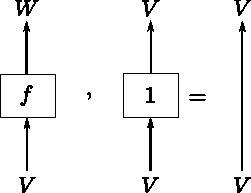
\includegraphics[scale=.8]{../assets/2518/wen_figures/morphisms.pdf}
\]
Tensor product of objects and morphisms will be denoted by horizontal juxtaposition:
\[
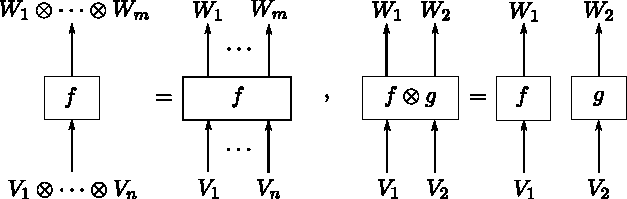
\includegraphics[scale=.8]{../assets/2518/wen_figures/tensors.pdf}
\]

\subsubsection{Duality}
For $V\in\mathcal{C}$, we~endow $V^*$ with the structure of a $\mathcal{U}$-module via
\[
x\cdot f(v)=f(S(x)v)
\]
for $x\in \mathcal{U}$, $f\in V^*$, and $v\in V$. We~set $(V\otimes W)^*= W^*\otimes V^*$ as they are isomorphic $\mathcal{U}$-modules under the natural tensor flip.
In our graphical calculus, we~will denote~$V^*$ using $V$ but use \textit{downward} pointing arrows.
Note that $V$ and $V^{**}$ are isomorphic under the \textit{nontrivial} isomorphism $S^2$.
It is easy to see that
\[
S^2(x) = \ad_{q^{2\rho}}(x).
\]
Since $\Delta(q^{2\rho})= q^{2\rho}\otimes q^{2\rho}$, we~can use $q^{2\rho}: V\to V^{**}$ to identify the two modules in a manner that respects tensor products. We~will do so and write $V$ instead of $V^{**}$, which will always imply a twist by $q^{-2\rho}$.

\subsubsection{Evaluation and coevaluation}
Let $\{ v_i\}$ be a basis of $V$ with corresponding dual basis $\{ v^i\}$ and let $\mathbbm{1}\in\mathcal{C}$ be the trivial representation.
The canonical maps
\begin{align*}
c&\mto cv_i\otimes v^i\in V\otimes V^*,\\
V^*\otimes V\ni v^i\otimes v_j&\mto \delta_{ij},
\end{align*}
are homomorphisms $\mathrm{coev}_V:\mathbbm{1}\to V\otimes V^*$ and $\mathrm{ev}_V:V^*\otimes V\to\mathbbm{1}$, respectively.
If $V$ is irreducible, they are the unique such homomorphisms.
Graphically, we~will omit depicting $\mathbbm{1}$; $\mathrm{ev}_V$ and $\mathrm{coev}_V$ appear as caps and cups oriented towards the left:
\[
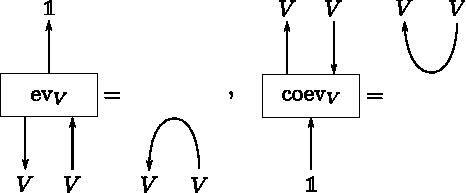
\includegraphics[scale=.8]{../assets/2518/wen_figures/cupcap.pdf}
\]

The ordering of tensor factors matters in $\mathrm{ev}_V$ and $\mathrm{coev}_V$.
To define maps with the opposite ordering, we~will use $q^{2\rho}$ to identify $V$ and $V^{**}$.
\begin{align*}
c&\mto cv^i\otimes q^{-2\rho}v_i\in V^*\otimes V,\\
V\otimes V^*\ni q^{-2\rho}v_i\otimes v^j&\mto \delta_{ij}.
\end{align*}
We denote these maps by $\mathrm{qcoev}_V$ and $\mathrm{qev}_V$, respectively.
Graphically, they will be depicted as cups and caps with orientations opposite from before:
\[
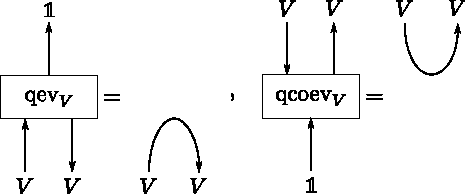
\includegraphics[scale=.8]{../assets/2518/wen_figures/qcupcap.pdf}
\]

\subsubsection{Adjunction}
The caps and cups allow us to define (right) adjoints.
For a morphism $f:V\to W$, $f^*:W^*\to V^*$ is given by
\[
f^*:=(\mathrm{ev}_W\otimes 1_{V^*})(1_{W^*}\otimes f\otimes 1_{V^*})(1_{W^*}\otimes\mathrm{coev}_V)
\]
\[
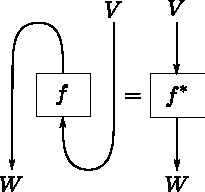
\includegraphics[scale=.8]{../assets/2518/wen_figures/adjoint.pdf}
\]
Note that the adjoint of the identity map of $V$ is the identity map of $V^*$.

\subsubsection{Braiding}
We will depict $\beta_{V,W}$ and $\beta_{V,W}^{-1}$ as braid crossings:
\[
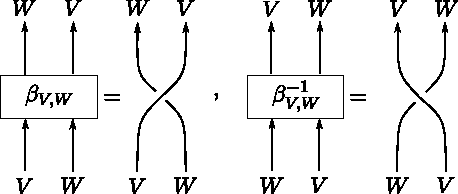
\includegraphics[scale=.8]{../assets/2518/wen_figures/braid.pdf}
\]
The quantum Yang-Baxter equation \eqref{YangBaxter} implies that $\beta_{V,W}$ endows $\mathcal{C}$ with the structure of a braided monoidal category.

\subsubsection{Ribbon structure}
By \eqref{DrinEle}, $u$ gives an isomorphism $V\to V^{**}$ and thus $q^{-2\rho}u$ is an automorphism of $V$, \ie it is central. We~define the \textit{ribbon element} $\nu$ by
\[
\nu := \left(q^{-2\rho}u\right)^{-1}=u^{-1}q^{2\rho}.
\]
Formula \eqref{DrinCo} implies that $\nu$ satisfies
\begin{equation}
\Delta(\nu)=\mathcal{R}_{21}\mathcal{R}(\nu\otimes\nu).
\label{RibbonCo}
\end{equation}
The following was computed in \cite{DrinAlmost}:
\begin{prop}\label{DrinProp}
On $V_\lambda$, $u$ acts as $q^{-\langle\lambda,\lambda+2\rho\rangle}q^{2\rho}$.
Thus, the ribbon element $\nu$ acts by the scalar $q^{\langle\lambda,\lambda+2\rho\rangle}$.
\end{prop}
Using \eqref{DrinInv}, we~can see that $\nu$ can be drawn in two ways:
\begin{equation}
\begin{array}{c}
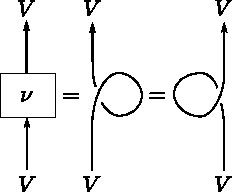
\includegraphics[scale=.8]{../assets/2518/wen_figures/ribbon.pdf}
\end{array}
\label{ribbonloop}
\end{equation}
Correspondingly, we~note that $\nu^{-1}$ can also be drawn in two ways:
\begin{equation}
\begin{array}{c}
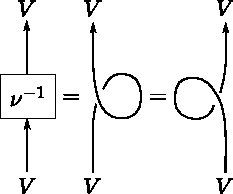
\includegraphics[scale=.8]{../assets/2518/wen_figures/ribboninv.pdf}
\end{array}
\label{ribbonloopinv}
\end{equation}

It is not quite true that morphisms in $\mathcal{C}$ only depend on the isotopy type of its diagram in $\RR^3$ under the graphical calculus.
Rather, we~should view each strand as a ribbon with a front side and back side, and we require the front side to always face the reader at the start and end of the ribbon.
The back side may appear in the middle if the loop given by $\nu$ appears, in~which case the ribbon in twisted twice.
Our graphical calculus assigns to each morphism in $\mathcal{C}$ a \textit{$\mathcal{C}$-colored ribbon tangle}.
\begin{thm}[\cite{ReshTurRibbon}]
A morphism in $\mathcal{C}$ only depends on the isotopy type of its associated tangle.
\end{thm}
We refer the reader to the original source as well as \cite{BakKir} for details.
In practice, we~will instead work with strands but keep track of loops representing $\nu$.

\subsection{Reflection equation algebra}
Here, we~introduce a quantization of the Hopf algebra of functions on $\GL_n$. We~would like this Hopf algebra to be a $\mathcal{U}=\rU_q(\mathfrak{gl}_n)$-module, and, critically, we~want its structure maps to be $\UU$-homomorphisms.
This requires a braided variant of Tannakian reconstruction, defined by Majid \cite{MajidBraided}.
The resulting algebra is a localization of what is known as the \textit{reflection equation algebra}.

\subsubsection{Majid reconstruction}
Recall that $\mathcal{C}$ is the category of finite-dimensional $\UU$-modules with weights in $P$. We~define the $\UU$-module $\OO$ as a space of matrix elements:
\begin{equation}
\OO:=\Bigl(\bigoplus_{V\in\mathcal{C}}V^*\otimes V \Bigr)\Bigm/\Bigl\langle f^*(w^*)\otimes v-w^*\otimes f(v)\Bigm|
\begin{array}{l}
v\in V, w^*\in W^*,\\
f\in\mathrm{Hom}_{\GL_n}(V,W)
\end{array}
\Bigr\rangle.
\label{Coend}
\end{equation}
For the categorically-minded, $\OO$ is the \textit{coend} of the identity functor of $\mathcal{C}$.
By considering for $f$ in \eqref{Coend} the projections onto irreducible representations, we~obtain an analogue of the Peter--Weyl Theorem:
\begin{equation}
\OO=\bigoplus_{\lambda\in P^+} V_\lambda^*\otimes V_\lambda.
\label{qPeterWeyl}
\end{equation}
As we will see below, we~can use operations on representations to define a Hopf algebra structure on $\OO$ that recovers at $q=1$ the classical Hopf algebra structure on the ring of functions on $\GL_n$.

\begin{itemize}
\item \textit{Coalgebra structure:}
The coalgebra structure is identical to that of the classical case.
For $v^*\otimes v\in V^*\otimes V$, we~define the coproduct $\nabla(v^*\otimes v)$ as
\begin{gather*}
\nabla(v^*\otimes v)=v^*\otimes \mathrm{coev}_V(1)\otimes v
\\
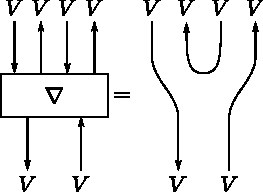
\includegraphics[scale=.8]{../assets/2518/wen_figures/coproduct.pdf}
\end{gather*}
The evaluation map $\mathrm{ev}_V$ on $V^*\otimes V$ yields the counit.
\item \textit{Algebra structure:}
In the classical case, the product structure entails permuting tensorands.
To make such an operation a $\UU$-morphism, we~utilize the braiding.
For $v^*\otimes v\in V^*\otimes V$ and $w^*\otimes w\in W^*\otimes W$,
\begin{gather}
m(v^*\otimes v\otimes w^*\otimes w) = \tensor[]{r}{_t}\tensor[]{r}{_s}w^*\otimes \tensor[_t]{r}{}v^*\otimes\tensor[_s]{r}{}v\otimes w
\label{TwistProd}
\\ \notag
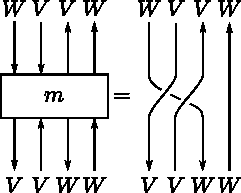
\includegraphics[scale=.8]{../assets/2518/wen_figures/product.pdf}
\end{gather}
The inclusion $\mathbbm{1}\to\mathbbm{1}^*\otimes\mathbbm{1}\in\OO$ provides the unit.
\item \textit{Antipode:} The antipode $\iota$ is given by
\begin{gather}
\iota(v^*\otimes v)= \nu \tensor[]{r}{_s} v\otimes \tensor[_s]{r}{}v^*
\label{Antipode}
\\ \notag
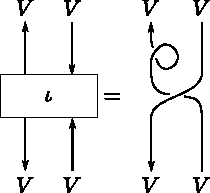
\includegraphics[scale=.8]{../assets/2518/wen_figures/antipode.pdf}
\end{gather}
We note that the relations for the coend \eqref{Coend} are necessary to show that $\iota$ is an antipode.
For example, in~computing $m\circ(1\otimes\iota)\circ\nabla$, we~use the coend relation in the first equality below:
\[
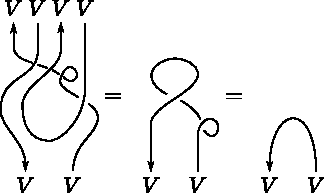
\includegraphics[scale=.8]{../assets/2518/wen_figures/antirel.pdf}
\]
In the last equality, recall that $\nu$ and $\nu^{-1}$ each have two diagrammatic presentations, given by \eqref{ribbonloop} and \eqref{ribbonloopinv}, respectively.
\end{itemize}

\subsubsection{Generating matrix}\label{RMatrixRE}
Since the finite-dimensional representations of $\mathcal{U}$ can be built out of tensor functors applied to the vector representation $\mathbb{V}$, it is perhaps unsurprising that $\OO$ has a presentation written in terms of matrix elements of $\mathbb{V}$.
The generators of this presentation are a set of symbols $\left\{ m_{j}^i\, |\, i,j=1,\ldots n \right\}$. We~arrange them into a matrix $M=(M_{j}^i)$ where
\[
M^i_j=E_j^i\otimes m^i_j.
\]
\begin{defn}\label{REAlgDef}
The \textit{reflection equation algebra} $\mathfrak{R}$ is generated by $\left\{ m^i_j \right\}$ and has relations
\begin{equation}
R_{21}M_{13}R_{12}M_{23}=M_{23}R_{21}M_{13}R_{12}.
\label{RE}
\end{equation}
\end{defn}

\begin{thm}[\cite{DonMudRET}]
The map $m_j^i\mto e^i\otimes e_j$ gives an embedding from $\mathfrak{R}$ to~$\OO$.
It is an isomorphism after inverting a central element of $\mathfrak{R}$ called the quantum determinant $\det_q(M)$, which is mapped to $\mathrm{qcoev}_{\mathbbm{1}_1}(1)$.
\end{thm}
Equation \eqref{RE} is known as the \textit{reflection equation}.
For an explicit formula for the quantum determinant, see \cite{JorWhite}.

We will abuse notation and conflate $\mathfrak{R}$ with its image in $\OO$.
Let $M^{-1}:=(1\otimes\iota)(M)$.
By the definition of the antipode, we~have:
\[
M^{-1}M=MM^{-1}=I.
\]
\begin{cor}\label{REInv}
$\OO$ is generated by $\det_q(M)$ and the entries of $M^{-1}$.
\end{cor}

\begin{proof}
First, note that
\begin{gather*}
\textstyle\iota(\det_q(M))=\iota^{-1}(\det_q(M))=\det_q(M)^{-1}
\\
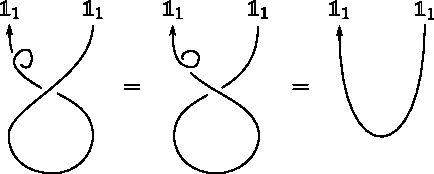
\includegraphics[scale=.8]{../assets/2518/wen_figures/detinv.pdf}
\end{gather*}
Thus, by writing $\det_q(M)$ in terms of the entries of $M$ and applying $\iota$, we~obtain an expression for $\det_q(M)^{-1}$ in terms of the entries of $M^{-1}$.
Similarly, we~can write the entries of $(1\otimes \iota^{-1})(M)$ in terms of the entries of $M$ and $\det_q(M)^{-1}$.
Applying $\iota$, we~obtain an expression for the entries of $M$ in terms of those of $M^{-1}$ and $\det_q(M)$.
\end{proof}

\subsubsection{Killing form}\label{Kill}
Matrix elements give functionals on $\UU$ in the natural way: for $v^*\otimes v\in V^*\otimes V$ and $x\in \UU$:
\[
(v^*\otimes v)(x)=v^*(xv).
\]
A quantum analogue of the Killing form would allow us to view matrix elements as sitting inside the enveloping algebra.
The canonical tensor for such a form is given by $\mathcal{R}_{21}\mathcal{R}$.
\begin{thm}[\cite{JosLetztLocal}]\label{KappaThm}
The map $\kappa:\OO\to \mathcal{U}$ given by
\[
\kappa(v^*\otimes v)=((v^*\otimes v)(-)\otimes 1)\mathcal{R}_{21}\mathcal{R}
\]
is a $\mathcal{U}$-equivariant algebra embedding, where $\mathcal{U}$ is endowed with the adjoint action.
\end{thm}

Observe that the map $V^*\otimes V\otimes W\to W$ given by
\[
v^*\otimes v\otimes w\mto \kappa(v^*\otimes v)(w)
\]
is the morphism in $\mathcal{C}$ depicted by the following diagram:
\[
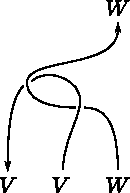
\includegraphics[scale=.8]{../assets/2518/wen_figures/kappa1.pdf}
\]

We will depict $\kappa(\OO)$ by replacing the strand for $W$ above by a dotted line oriented upwards---a ``ghost strand''.
Our graphical calculus is still valid for such strands because it holds for any choice of representation $W$ ``filling in'' the ghost strand; by the quantum analogue of a theorem of Harish-Chandra \cite{HCLie}, any $x\in\UU$ that acts trivially on all $W\in\mathcal{C}$ is necessarily zero.
Multiplying left-to-right in $\kappa(\OO)$ corresponds to stacking ghost strands top-to-bottom.
For example, that $\kappa$ is an algebra map follows from the manipulation below:
\[
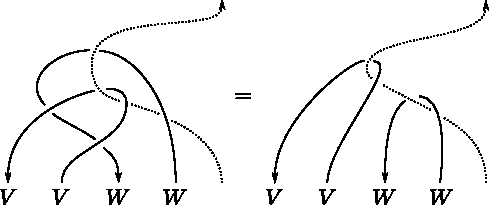
\includegraphics[scale=.8]{../assets/2518/wen_figures/kappa2.pdf}
\]
Finally, it can be useful to know that $\kappa\circ\iota$ yields the opposite crossing:
\[
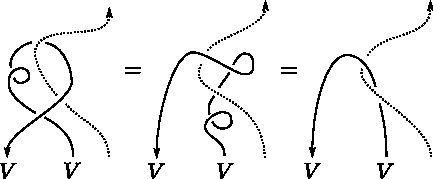
\includegraphics[scale=.8]{../assets/2518/wen_figures/kappainv.pdf}
\]

Theorem \ref{KappaThm} omits any statement about coalgebra structures because $\kappa$ does not intertwine $\nabla$ with $\Delta$.
By considering the action of $\kappa(v^*\otimes v)$ on a tensor product of modules, we~see that $\Delta\circ\kappa$ merely doubles the dotted strand. We~can force an instance of $\kappa$ for each dotted strand using $\nabla$ and some braidings:
\[
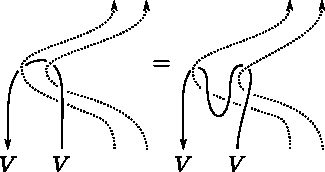
\includegraphics[scale=.8]{../assets/2518/wen_figures/kappa3.pdf}
\]
Properly comprehending the diagram on the right, we~get:

\begin{prop}[\protect{\cite[Ex.\,1.3.3(c)]{VarVassRoot}}]\label{Coideal}
Let $\left\{ v_i \right\}\subset V$ and $\left\{ v^i \right\}\subset V^*$ be dual bases.
For $v^*\otimes v\in V^*\otimes V$, we~have
\begin{equation}
(\Delta\circ\kappa)(v^*\otimes v)= \kappa(v^*\otimes v_i)\tensor[]{r}{_s}\tensor[]{r}{_t}\otimes\kappa(\tensor[_s]{r}{}v^i\otimes\tensor[_t]{r}{}v).
\label{DeltaKappa}
\end{equation}
In particular, $\kappa(\OO)$ is a left coideal subalgebra of $\mathcal{U}$, \ie
\begin{align*}
(\Delta\circ\kappa)(\OO)&\subset \mathcal{U}\otimes\kappa(\OO).
\end{align*}
\end{prop}

\subsection{Etingof--Kirillov theory}\label{EtKirThy}
Equipped with a notion of functions on quantum $\GL_n$, we~move on to a realization of Macdonald polynomials as spherical functions on the quantum group.
This was discovered by Etingof and Kirillov, Jr. \cite{EtKirQuant}. We~conclude this section by making contact with $\SHH_n(q,q^k)$.

\subsubsection{Traces of intertwiners}
Let $U\in\mathcal{C}$. We~will be concerned with the space of homomorphisms
\[
I(V_\lambda, U):=\mathrm{Hom}_{\mathcal{U}}(V_\lambda,V_\lambda\otimes U)
\]
also called \textit{intertwiners}.
Let $v_\lambda\in V_\lambda$ be a highest weight vector and $U[0]$ denote the zero weight space.
For an intertwiner $\Phi$, set
\[
\langle\Phi\rangle=(v_\lambda^*\otimes 1_U)\Phi(v_\lambda)\in U[0].
\]
\begin{prop}[\cf 3.1 in \cite{EtLatBook}]\label{IntHigh}
The map $\Phi\mto\langle\Phi\rangle$ is an injective map $I(V_\lambda,U)\hto U[0]$.
\end{prop}

To extract a Laurent polynomial from this, we~take the weighted trace over $V_\lambda$:
\[
\Phi\mto\varphi:=\mathrm{tr}_{V_\lambda}(\Phi(q^{2\mu})).
\]
Viewing this as a function of $\mu\in P$ and setting $x_i=q^{2\langle\epsilon_i,-\rangle}$, we~obtain a Laurent polynomial in the variables $\{ x_i \}_{i=1}^n$ valued in $U[0]$.
From Proposition \ref{IntHigh}, it follows that the trace map is injective because the intertwiner is determined by the coefficient of $x_1^{\lambda_1}\cdots x_n^{\lambda_n}$.

We would prefer to work instead with what can be called $U$-spherical functions on quantum $\GL_n$.
This amounts to applying quantum coevaluation maps:
\begin{align*}
I(V_\lambda, U)&\cong (V_\lambda^*\otimes V_\lambda\otimes U)^{\mathcal{U}}\\
\Phi&\mto(1_{V_\lambda^*}\otimes\Phi)\circ(\mathrm{qcoev}_{V_{\lambda}})=:\tensor[_\cup]{\Phi}{}
\end{align*}
\[
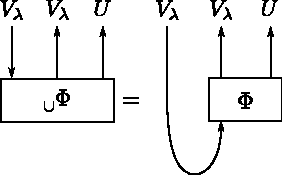
\includegraphics[scale=.8]{../assets/2518/wen_figures/Twine1.pdf}
\]
Since $q^{2\rho}$ and $q^{2\mu}$ are both group like, we~have
\begin{equation}
\varphi=(\mathrm{ev}_{V_\lambda}\otimes 1_U)\bigl((q^{-2\mu-2\rho}\otimes 1_{V_{\lambda}\otimes U})\tensor[_\cup]\Phi{}\bigr).
\label{TraceSphere}
\end{equation}
This has a clear graphical interpretation in terms of closing the loop between the~$V_\lambda$ strands, but we will refrain from drawing it as the insertion of $q^{-2\mu}$ breaks $\UU$\nobreakdash-equi\-variance.

\subsubsection{Macdonald polynomials revisited}
Now, fix $k\in\ZZ_{\ge 0}$. We~will consider the case
\[
U=\rU_k:=S_q^{n(k-1)}\mathbb{V}\otimes\mathbbm{1}_{-(k-1)}.
\]
$\rU_k[0]$ is one-dimensional, spanned by the vector whose tensorand in $S_q^{nk}\mathbb{V}$ is the $q$\nobreakdash-symmetrization of
\[
\left(e_1\otimes e_2\otimes\cdots\otimes e_n\right)^{\otimes{k-1}}.
\]
Fixing a vector $u_0\in \rU_k[0]$, we~can identify $\rU_k[0]$ with $\CC(q)$.
Recall that\vspace*{-3pt}
\[
\delta=(n-1,n-2,\ldots, 0).
\]

\begin{thm}[\cite{EtKirQuant}]\label{EtKirMac}
We have the following:
\begin{enumerate}
\item\label{EtKirMac1} For $\lambda\in P^+$, $I(V_\lambda,\rU_k)$ is nonzero if and only if $\lambda-(k-1)\delta$ is dominant.
For $\lambda\in P^+$, set\vspace*{-3pt}
\[
V_\lambda^k:=V_{\lambda+(k-1)\delta}.
\]
Thus, for $\lambda\in P^+$, there exists a unique nonzero intertwiner\vspace*{-3pt}
\[
\Phi^{k}_\lambda:V_{\lambda}^k\to V_{\lambda}^k\otimes \rU_{k}
\]
with $\langle\Phi^{k}_\lambda\rangle=u_0$.
\item\label{EtKirMac2} Let $\varphi^{k}_\lambda$ be the weighted trace $\mathrm{tr}_{V_{\lambda}}(\Phi^k_\lambda(q^{2\mu}))$. We~have:\vspace*{-3pt}
\[
P_\lambda(q, q^{k})=\varphi^k_{\lambda}\big/\varphi^k_{0}.
\]
\end{enumerate}
\end{thm}

\subsubsection{Spherical DAHA generators}\label{EtKirDAHA}
Recall the generators of $\SHH_n(q,q^k)$ from Lemma \ref{GenLem} (\cf also \eqref{DAHADet} and \eqref{ElemXY}). We~have two natural actions of $\OO^\UU$ on the Macdonald polynomials.
Let $\mathrm{ch}_{V_{\pi}}$ denote the character of $V_\pi$.
The first action is through insertion via $\kappa$:

\begin{thm}[\cite{EtKirQuant}]
We have
\[
\Phi^k_{\lambda}(\kappa(\mathrm{qcoev}_{V^*_\pi}(1))-)=q^{-|\pi|(n-1)}\mathrm{ch}_{V_{\pi}}(q^{2(\lambda+k\delta)})\Phi_{\lambda}^k.
\]
\end{thm}

This induces the same action on the weighted trace.
In terms of spherical functions, this corresponds to:\vspace*{-3pt}
\[
(\kappa(\mathrm{qcoev}_{V_\pi}(1))\otimes 1_{V_{\lambda}\otimes \rU_k})\tensor[_\cup]{\Phi}{}_{\lambda}^k=q^{-|\pi|(n-1)}\mathrm{ch}_{V_{\pi}}(q^{2(\lambda+k\delta)})\tensor[_\cup]{\Phi}{}_\lambda^k
\]
\[
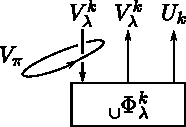
\includegraphics[scale=.8]{../assets/2518/wen_figures/Twine2.pdf}
\]
Note that the discrepancy between $V_\pi$ and $V_\pi^*$ comes from the change in orientation on the circle when bending the left leg of $\tensor[_\cup]{\Phi}{}_\lambda^k$ down to obtain $\Phi_\lambda^k$.
In particular, we~obtain the $q^{-r(n-1)}\rrr\left(\ee e_r(\boldsymbol{Y}_n^{-1})\ee \right)$ when $V_\pi=\wedge_q^r\mathbb{V}^*$ and $q^{-n(n-1)}\rrr(\ee \boldsymbol{Y}_n\ee)$ when $V_\pi=\mathbbm{1}_1$.

For the second action, consider the multiplication map:\vspace*{-3pt}
\[
m\otimes 1_{\rU_k}:\OO\otimes\OO\otimes \rU_k\to \OO\otimes \rU_k.
\]
Since it is a $\mathcal{U}$-homomorphism, it restricts to a map\vspace*{-3pt}
\[
\OO^\UU\otimes (\OO\otimes \rU_k)^{\mathcal{U}} \to (\OO\otimes \rU_k)^{\mathcal{U}} = \bigoplus_{\lambda\in P^+} (V_\lambda^*\otimes V_\lambda\otimes \rU_k)^{\mathcal{U}}.
\]
We can depict $(m\otimes 1_{\rU_k})(\mathrm{qcoev}_{V_\pi}(1)\otimes \tensor[_\cup]{\Phi}{}_\lambda^k)$ diagrammatically as:
\[
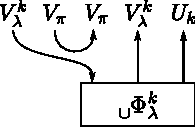
\includegraphics[scale=.8]{../assets/2518/wen_figures/Twine3.pdf}
\]
Converting to the weighted trace as in \eqref{TraceSphere} yields $\mathrm{ch}_{V_\pi}(x_1,\ldots x_n)\varphi_\lambda^k$.
Here, we~obtain $\rrr\left(\ee e_r(\boldsymbol{X}_n)\ee \right)$ when $V_\pi=\wedge_q^r\mathbb{V}$ and $\rrr\left(\ee \boldsymbol{X}_n^{-1}\ee \right)$ when $V_\pi = \mathbbm{1}_{-1}$.

\section{Quantum differential operators}

\subsection{Varagnolo--Vasserot double}\label{QDO}
Out of our quantum ring of functions $\OO$, we~would like to define a notion of quantum differential operators with very specific equivariance properties.
Let us catalog the $\mathcal{U}$-actions on $\OO$:
\begin{enumerate}
\item \textit{Left coregular action:} $g\triangleright(v^*\otimes v)=gv^*\otimes v$ (this is an action of the co-opposite $\mathcal{U}_c$);
\item \textit{Right coregular action:} $g\triangleleft(v^*\otimes v)=v^*\otimes gv$;
\item \textit{Coadjoint action:} $g\bowtie(v^*\otimes v)=g_{(1)}v^*\otimes g_{(2)}v$.
\end{enumerate}
We have been mainly concerned with the coadjoint action, for which the Hopf algebra structure maps are homomorphisms.
Our goal is to construct a smash product between~$\OO$ and $\kappa(\OO)$ utilizing the left coregular action, but we would like all structure maps to be equivariant with respect to the coadjoint action on $\OO$ and the adjoint action on~$\kappa(\OO)$.

\subsubsection{Drinfeld twist}
The left and right coregular actions give an action of $\UU_c\otimes\UU$ on $\OO$.
However, the braidings in \eqref{TwistProd} prevent the product from being a $\UU_c\otimes\UU$-homomorphism.
This can be fixed by altering the coproduct of $\UU_c\otimes\UU$ using Drinfeld's twisting procedure \cite{DrinQuasi}.
First, let $\Delta_2$ denote the coproduct of $\UU_c\otimes\UU$:
\[
\Delta_2(g\otimes h)=g_{(2)}\otimes h_{(1)}\otimes g_{(1)}\otimes h_{(2)}.
\]
Let $\widetilde{\UU}^2$ denote the algebra $\UU_c\otimes\UU$ endowed with coproduct
\begin{align*}
\widetilde{\Delta}_2(g\otimes h)&:=(\mathcal{R}_{13}\mathcal{R}_{23})^{-1}\Delta_2(g\otimes h)(\mathcal{R}_{13}\mathcal{R}_{23})\\
&\hphantom{:}= \mathcal{R}_{23}^{-1}(g_{(1)}\otimes h_{(1)}\otimes g_{(2)}\otimes h_{(2)})\mathcal{R}_{23}
\intertext{and antipode}
\widetilde{S}_2(g\otimes h)&=\mathcal{R}_{21}\big(S(g)\otimes S(h)\big)\mathcal{R}_{21}^{-1}.
\end{align*}
With these structures, $\widetilde{\UU}^2$ is a Hopf algebra in a suitably completed sense. We~will use an embellished Sweedler notation for $\widetilde{\Delta}_2$:
\[
\widetilde{\Delta}_2(g\otimes h)=\tilde{g}_{(1)}\otimes\tilde{h}_{(1)}\otimes\tilde{g}_{(2)}\otimes\tilde{h}_{(2)}.
\]

\begin{prop}
The multiplication map $m$ of $\OO$ is a $\widetilde{\UU}^2$-homomorphism.
\end{prop}

\begin{proof}
This follows from the calculation:
\begin{align*}
&m\bigl(\widetilde{\Delta}_2(g\otimes h)(v^*\otimes v\otimes w^*\otimes w)\bigr)\\
&=\beta_{V^*\otimes V, W^*}\bigl(\mathcal{R}_{23}^{-1}(g_{(1)}v^*\otimes h_{(1)}\tensor[_s]{r}{} v\otimes g_{(2)}\tensor[]{r}{_s}w^*\otimes h_{(2)}w)\bigr)\\
&=\tensor[]{r}{_t}g_{(2)}\tensor[]{r}{_s}w^*\otimes \tensor[_t]{r}{} g_{(1)}v^*\otimes h_{(1)}\tensor[_s]{r}{}v\otimes h_{(2)}w\\
&=g_{(1)}\tensor[]{r}{_t}\tensor[]{r}{_s}w^*\otimes g_{(2)}\tensor[_t]{r}{}v^*\otimes h_{(1)}\tensor[_s]{r}{}v\otimes h_{(2)}w\\
&=(g\otimes h)m(v^*\otimes v\otimes w^*\otimes w).\qedhere
\end{align*}
\end{proof}

\subsubsection{Three embeddings}
Corresponding to the three actions of $\UU$ on $\OO$, there are three embeddings of $\UU$ into $\widetilde{\UU}^2$.
First, let us consider the subalgebras $\UU\otimes 1$ and $1\otimes\UU$.
It is clear that the restrictions of the $\widetilde{\UU}^2$-action on $\OO$ to these two subalgebras respectively yield the left and right coregular actions. We~have that\vspace*{-3pt}
\begin{equation}
\begin{aligned}
\widetilde{\Delta}_2(g\otimes 1)&=g_{(1)}\otimes \tensor[_s]{r}{}\tensor[_t]{r}{}\otimes S(\tensor[]{r}{_s})g_{(2)}\tensor[]{r}{_t}\otimes 1\\
&= g_{(1)}\otimes \tensor[_s]{r}{}\otimes \ad_{S(\tensor[]{r}{_s})} (g_{(2)})\otimes 1.
\end{aligned}
\label{SubCoproductL}
\end{equation}
Thus, $\UU\otimes 1$ is a left coideal subalgebra, and so by Theorem \ref{KappaThm} and Proposition \ref{Coideal}, $\kappa(\OO)\otimes 1$ is a left coideal subalgebra as well.

Next, view the coproduct as a map $\Delta:\UU\to\widetilde{\UU}^2$.
Observe that by \eqref{RMatrixCo},\vspace*{-3pt}
\begin{align}
\nonumber
(\widetilde{\Delta}_2\circ\Delta)(g)&=g_{(1)}\otimes g_{(2)}\otimes g_{(3)}\otimes g_{(4)},\\
\label{TildeAdjoint}
(1\otimes\widetilde{S})(\widetilde{\Delta}_2\circ\Delta)(g)&=g_{(1)}\otimes g_{(2)}\otimes S(g_{(4)})\otimes S(g_{(3)}).
\end{align}
From these equations, we~can see that $\Delta$ is in fact a Hopf algebra morphism.
Moreover, from \eqref{TildeAdjoint}, we~can see that the adjoint action of $\Delta(\UU)$ on $\widetilde{\UU}^2$ preserves $\UU\otimes 1$, on which it acts by the usual adjoint action on $\UU$.

\subsubsection{Smash product}
Now consider the smash product $\OO\rtimes\widetilde{\UU}^2$.
This is the tensor product $\OO\otimes\widetilde{\UU}^2$ subject to the relation that for $v^*\otimes v\in\OO$ and $g\otimes h\in\widetilde{\UU}^2$,\vspace*{-3pt}
\begin{equation}
(g\otimes h)(v^*\otimes v)=(\tilde{g}_{(1)}v^*\otimes\tilde{h}_{(1)}v)(\tilde{g}_{(2)}\otimes\tilde{h}_{(2)}).
\label{SmashProdDef}
\end{equation}
We will abuse notation and use $\OO$ and $\widetilde{\UU}^2$ to denote $\OO\otimes 1\otimes 1$ and $1\otimes \widetilde{\UU}^2$, respectively.
Since $\kappa(\OO)\otimes 1\subset\widetilde{\UU}^2$ is a left coideal, the subspace $\OO\rtimes(\kappa(\OO)\otimes 1)$ is in fact a subalgebra. We~denote by $\partial_\triangleright$ the embedding $\OO\to1\otimes\kappa(\OO)\otimes 1\subset\OO\rtimes\widetilde{\UU}^2$.

\begin{defn}[\cite{VarVassRoot}]
The \textit{Varagnolo--Vasserot algebra of quantum differential operators} $\DD$ is the subalgebra $\OO\rtimes\partial_\triangleright(\OO)$ of the smash product $\OO\rtimes\widetilde{\UU}^2$.
\end{defn}

The Varagnolo--Vasserot algebra does indeed satisfy our desired equivariance.
Letting $\widetilde{\UU}^2$ act on itself via the adjoint action, $\OO\rtimes\widetilde{\UU}^2$ is a $\widetilde{\UU}^2$-module-algebra.
Restricting this action to $\Delta(\UU)\subset\widetilde{\UU}^2$, we~obtain an action of $\UU$ on $\DD$ that gives the coadjoint action on $\OO$ and the adjoint action on $\partial_\triangleright(\OO)$. We~will also use $\bowtie$ to denote this $\UU$ action on $\DD$.

Finally, we~note that by \eqref{SubCoproductL}, commuting $\partial_\triangleright(\OO)$ past $\OO$ in $\DD$ does not cleanly incorporate the left coregular action because the right tensorand of $\OO$ is also affected.
However, the discrepancy has a diagrammatic interpretation that is cleaner than the symbolic formula gotten by combining \eqref{DeltaKappa} and \eqref{SubCoproductL}:
\begin{gather}
\partial_\triangleright(v^*\otimes v)(w^*\otimes w)= \big(\partial_\triangleright(v^*\otimes v_i)\tensor[]{r}{_s}\tensor[]{r}{_t} w^*\otimes \tensor[_u]{r}{}\tensor[_v]{r}{}w\big)\big(S(\tensor[]{r}{_u})\partial_\triangleright(\tensor[_s]{r}{}v^i\otimes\tensor[_t]{r}{}v)\tensor[]{r}{_v}\big)\notag
\\
\begin{array}{c}
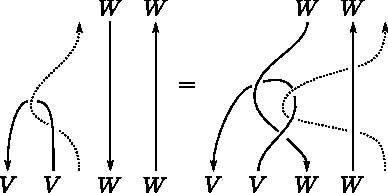
\includegraphics[scale=.7]{../assets/2518/wen_figures/smash.pdf}
\end{array}
\label{Smash}
\end{gather}

\subsubsection{Basic representation}
The smash product $\OO\rtimes\widetilde{\UU}^2$ has an action on $\OO$, where~$\OO$ acts by multiplication and $\widetilde{\UU}^2$ acts via the left and and right coregular actions.
This action is $\widetilde{\UU}^2$-equivariant.
Moreover, from the definition of the smash product \eqref{SmashProdDef}, we~have that $\OO$ is an induced representation:
\begin{equation}
\OO\cong\OO\rtimes\widetilde{\UU}^2\big/\OO\rtimes\widetilde{\UU}^2\bigl(\widetilde{\UU}^2-\epsilon(\widetilde{\UU}^2)\bigr).
\label{BasicRep}
\end{equation}
We call the representation $\OO$ and its restriction to $\DD$ the \textit{basic representation}.
$\OO$ is then a $\UU$-equivariant $\DD$-module (using the $\bowtie$ action).
Note that even though the smash product relations do not cleanly incorporate the left coregular action, $\partial_{\triangleright}(\OO)$ does indeed act on $\OO$ via the left coregular action.
This follows from \eqref{SubCoproductL} and \eqref{BasicRep}.

\subsection{Monodromy matrices}
Recall the generating matrix $M$ for $\OO$ given in \ref{RMatrixRE}.
Let $\{a^i_j\}$ denote a copy of $\{m^i_j\}$ given by $\OO\subset\DD$ and let $\{b^i_j\}$ denote another copy given by $\{\partial_\triangleright(m^i_j)\}$. We~define the matrices $A$, $B$, $A^{-1}$, and $B^{-1}$ by:
\begin{align*}
A_j^i&= E_j^i\otimes a_j^i, & (A^{-1})^i_j&= E_j^i\otimes \iota(a^i_j),\\
B_j^i&= E_j^i\otimes b_j^i, & (B^{-1})_j^i&= E_j^i\otimes\iota(b^i_j):=E_j^i\otimes\partial_\triangleright(\iota(m^i_j)).
\end{align*}

\subsubsection{Determinant bigrading}\label{QDet}
We set:
\begin{align*}
\textstyle\det_q(A)&:=\mathrm{qcoev}_{\mathbbm{1}_1}(1)\otimes 1\in\OO\otimes 1\subset\DD,\\
\textstyle\det_q(B)&:=\partial_{\triangleright}\mathrm{qcoev}_{\mathbbm{1}_1}(1)\in 1\otimes\kappa(\OO)\subset\DD.
\end{align*}
As in \ref{RMatrixRE}, these elements can be written in terms of the entries of $A$ and $B$, respectively.
Moreover, $\det_q(A)$ commutes with $\OO\otimes 1$ and $\det_q(B)$ commutes with $1\otimes\kappa(\OO)$.
Their commutation relations with elements from their respective ``opposite'' tensor factors are also nice.

First note that, from the factorization \eqref{RFactor} and the formulas \eqref{DetForm} for the determinant representation, we~have:
\begin{equation}
\begin{array}{c}
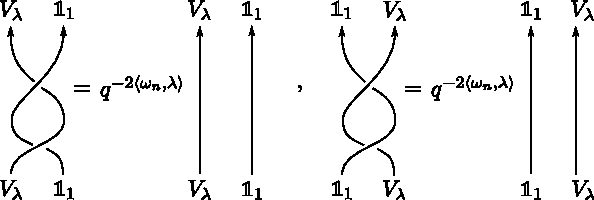
\includegraphics[scale=.8]{../assets/2518/wen_figures/detrel.pdf}
\end{array}
\label{detrel}
\end{equation}
Using these local relations on \eqref{Smash}, one can see that $\det_q(B)$ satisfies:
\[
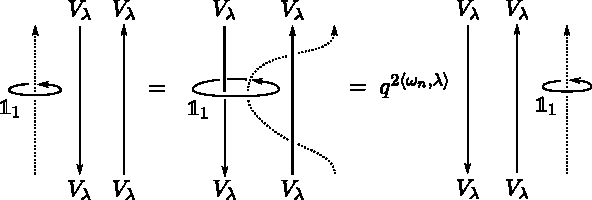
\includegraphics[scale=.8]{../assets/2518/wen_figures/detb.pdf}
\]
Similarly, $\det_q(A)$ satisfies:
\[
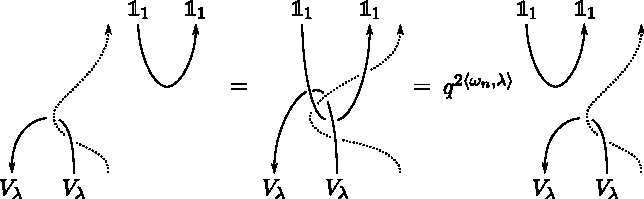
\includegraphics[scale=.8]{../assets/2518/wen_figures/deta.pdf}
\]
Thus, we~can define an internal bigrading on $\DD$: $x\in\DD$ is homogeneous of \hbox{degree}~$(a,b)$~if
\[
\textstyle\det_q(B)x=q^{2a} x\textstyle\det_q(B),\quad
\textstyle\det_q(A)x=q^{-2b} x\textstyle\det_q(A).
\]
The entries of $A$ and $B$ have degrees $(1,0)$ and $(0,1)$, respectively.

\subsubsection{Double R-matrix presentation}
The following is \cite[Prop.\,1.8.3(b)]{VarVassRoot}:

\begin{prop}\label{DoublePres}
Let $\DD_+$ be the algebra with generators given by the entries of $A$ and $B$ and relations
\begin{align}
\begin{split}
R_{21}A_{13}R_{12}A_{23}&=A_{23}R_{21}A_{13}R_{12},\\
R_{21}B_{13}R_{12}B_{23}&=B_{23}R_{21}B_{13}R_{12},\\
R_{21}B_{13}R_{12}A_{23}&=A_{23}R_{12}B_{13}R_{21}^{-1}.
\end{split}
\label{ABPres}
\end{align}
The elements $\{\det_q(A),\det_q(B)\}$ generate an Ore set in $\DD_+$ and $\DD$ is isomorphic to its localization.
\end{prop}

The novel third relation is a rewriting of \eqref{Smash}, \cf \cite[A.5]{VarVassRoot}.
This algebra was defined prior to \cite{VarVassRoot} by Alekseev and Schomerus \cite{AlekScho} as an intermediate step to constructing their quantized character variety for the once-punctured torus.
There, the $A$- and $B$-matrices respectively quantize monodromy matrices along the $a$- and $b$-cycles of the torus.

\subsection{Quantum Weyl algebra}\label{QWeyl}
A reference for this section is \cite{GiaZhaQW}.
The \textit{quantum Weyl algebra} of rank $n$, denoted $\WW$, is the $\CC(q)$-algebra with generators
\[
\left\{ \xi_i, \del_i\,|\, 1\le i\le n\right\}
\]
and relations
\begin{align}
\begin{split}
\xi_i\xi_j&= q\xi_j\xi_i\quad\text{for }i>j,\\
\del_i\del_j&=q^{-1}\del_j\del_i\quad\text{for }i>j,\\
\del_i\xi_j&=q\xi_j\del_i\quad\text{for }i\not=j,\\
\del_i\xi_i&=1+q^2\xi_i\del_i+(q^2-1)\sum_{j<i}\xi_j\del_j.
\end{split}\label{WeylPres}
\end{align}
If we set $\deg \xi_i=1$ and $\deg\del_i=-1$, then the relations \eqref{WeylPres} respect the grading. We~denote by $\WW_0$ the subalgebra of degree 0 elements.

\begin{rem}
In \cite{JordanMult}, there is a parameter $t$ that the author then sets to $t=1$ (\cf Remark 3.11 of loc.\,cit.).
Here, we~instead set $t=q^{-1}$.
This affects the formula for the moment map later in \ref{WMoment}.
\end{rem}

\subsubsection{Equivariance}
$\WW$ has an RTT-type presentation (\cf \cite[Ex.\,4.9]{JordanMult}): if we define the vectors
\begin{align*}
\vec{\xi}&:= \sum_{i=1}^n e^i\otimes \xi_i
=
\begin{pmatrix}
\xi_1 & \xi_2 & \cdots & \xi_n
\end{pmatrix}\!,
\\
\vec{\del}&:=\sum_{i=1}^ne_i\otimes \del_i
=
\begin{pmatrix}
\partial_1\\
\partial_2\\
\vdots\\
\partial_n
\end{pmatrix}
\end{align*}
in $\mathbb{V}\otimes\WW$ then relations \eqref{WeylPres} can be rewritten as
\begin{equation*}
\begin{aligned}
q\vec{\xi}_{13}\vec{\xi}_{23}&=\vec{\xi}_{23}\vec{\xi}_{13}R,\\
q\vec{\del}_{13}\vec{\del}_{23}&=R\vec{\del}_{23}\vec{\del}_{13},\\[-6pt]
q^{-1}\vec{\del}_{23}\vec{\xi}_{13}&=\vec{\xi}_{13}R\vec{\del}_{23}+q^{-1}\sum_{i=1}^n e^i\otimes e_i\otimes 1.
\end{aligned}
\end{equation*}
This algebra can be written as a quotient of the tensor algebra $\mathcal{T}(\mathbb{V}\oplus\mathbb{V}^*)$ by images of the braidings and evaluations.
Here, $\del_i$ corresponds to $e^i\in\mathbb{V}^*$ and $\xi_i$ corresponds to $e_i\in\mathbb{V}$.
Consequently, we~have:
\begin{prop}\label{WeylEquiv}
$\WW$ is a $\UU$-module-algebra.
\end{prop}
We denote the $\UU$-action on $\WW$ by $\bullet$.
Note that the degree is given by the action of $q^{\omega_n}$.
Since $q^{\omega_n}$ is central in $\UU$, it follows that $\WW_0$ is a $\UU$-submodule.

\subsubsection{Functional representation}
Let $\WW_{\xi}$ be the subalgebra generated by $\left\{ \xi_i \right\}$.
As~a $\UU$-module, the subalgebra $\WW_{\xi}$ is isomorphic to the \textit{quantum symmetric algebra} of~$\mathbb{V}$:
\[
S_q\mathbb{V}:=\bigoplus_{m=0}^\infty S_q^m\mathbb{V}.
\]
The ordered monomials
\[
\xi_1^{k_1}\cdots \xi_{n-1}^{k_{n-1}}\xi_n^{k_n}
\]
form a basis of $S_q\mathbb{V}$ (\cf Theorem \ref{JorBasis} below). We~can extend the natural multiplication action of $\WW_\xi$ to one of the entirety of $\WW$ by setting
\begin{equation*}
\del_i(\xi_1^{k_1}\xi_{2}^{k_{2}}\cdots \xi_{i}^{k_i}\cdots \xi_n^{k_n})=(q\xi_{1})^{k_{1}}(q\xi_{2})^{k_{2}}\cdots [k_i]_{q^2}\xi_i^{k_{i}-1}\xi_{i+1}^{k_{i+1}}\cdots \xi_n^{k_n}.
\end{equation*}
This action is merely the one induced by quotienting $\mathcal{T}(\mathbb{V}\oplus\mathbb{V}^*)$ by the left ideal generated by $\mathbb{V}^*$.
As such, this action is $\UU$-equivariant.
The action of $\WW_0$ on $S_q\mathbb{V}$ preserves each piece $S_q^m\mathbb{V}$.

\subsubsection{Difference operators}\label{WeylDiff}
It will be useful to interpret the functional representation in terms of difference operators in commuting variables.
Let
\[
\CC(q)[\boldsymbol{z}_n]:=\CC(q)[z_1,\ldots, z_n]
\]
and let $T_{q,z_i}$ denote the $q$-shift operator:
\[
T_{q,z_i}z_j=q^{\delta_{i,j}}z_j.
\]
For an integer vector $\lambda=(\lambda_1,\ldots,\lambda_n)\in\ZZ^n$, we~define
\[
z^\lambda:=z_1^{\lambda_1}\cdots z_n^{\lambda_n},\quad
T_\lambda:=T_{q,z_1}^{\lambda_1}\cdots T_{q,z_n}^{\lambda_n}.
\]
Consider the following rings of difference operators:
\begin{align*}
\mathbb{D}_q(\boldsymbol{z}_n)&= \Bigl\{ \textstyle\sum_{\lambda,\mu\in\ZZ^n}a_{\lambda,\mu}z^\lambda T_\mu\Bigm|
\begin{array}{l}
a_{\lambda,\mu}\in \CC(q) \\
\hbox{and only finitely many }a_{\lambda,\mu}\not=0
\end{array}
\Bigr\},\\
\mathbb{D}_q^+(\boldsymbol{z}_n)&= \Bigl\{ D\in \mathbb{D}_q(\boldsymbol{z}_n)\Bigm|
\begin{array}{l}
Df\in\CC(q)[\boldsymbol{z}_n]\\
\hbox{for all }f\in\CC(q)[\boldsymbol{z}_n]
\end{array}
\Bigr\}.
\end{align*}

\begin{prop}
$\CC(q)[\boldsymbol{z}_n]$ is a faithful representation of $\mathbb{D}_q^+(\boldsymbol{z}_n)$.
\end{prop}

The map
\[
\xi_1^{k_1}\cdots \xi_n^{k_n}\mto z_1^{k_1}\cdots z_n^{k_n}
\]
induces a vector space isomorphism $S_q\mathbb{V}\cong\CC(q)[\boldsymbol{z}_n]$.
Carrying over the actions of $\UU$ and $\WW$, we~obtain homomorphisms of both algebras into $\mathbb{D}_q^+(\boldsymbol{z}_n)$, both of which we denote by $\mathfrak{qdiff}$:
\begin{equation}
\begin{aligned}
\mathfrak{qdiff}(q^{\epsilon_i})&= T_{q,z_i},&
\mathfrak{qdiff}(\xi_i)&=z_i T_{q, z_1}\cdots T_{q,z_{i-1}},\\
\mathfrak{qdiff}(E_i)&= \frac{z_{i}}{z_{i+1}}\Bigl(\frac{T_{q,z_{i+1}}-T_{q, z_{i+1}}^{-1}}{q-q^{-1}} \Bigr),&
\mathfrak{qdiff}(\partial_i)&= z_i^{-1}T_{q,z_1}\cdots T_{q,z_{i-1}}\Bigl(\frac{T_{q,z_i}^2-1}{q^2-1} \Bigr),\\
\mathfrak{qdiff}(F_i)&= \frac{z_{i+1}}{z_i}\Bigl(\frac{T_{q,z_i}-T_{q, z_i}^{-1}}{q-q^{-1}} \Bigr).
\end{aligned}
\label{QDiffMap}
\end{equation}
Since $\CC(q)[\boldsymbol{z}_n]\cong S_q\mathbb{V}$ is a faithful $\mathbb{D}^+_q(\boldsymbol{z}_n)$-module, the fact that $S_q\mathbb{V}$ is a $\UU$-equivariant $\WW$-module implies that $\mathfrak{qdiff}$ pieces together into an algebra homomorphism out of the smash product:
\[
\mathfrak{qdiff}:\WW\rtimes\UU\to\mathbb{D}^+_q(\boldsymbol{z}_n).
\]

\subsection{Quantum Hamiltonian reduction}
To perform quantum Hamiltonian reduction, we~will need a notion of quantum moment maps in our Hopf-algebraic setting.
Let $H$ be a Hopf algebra acting on an algebra $A$ such that $A$ is an $H$-module-algebra.
If we denote this action by
\[
(-)\blacktriangleright(-):H\otimes A\to A,
\]
then a \textit{quantum moment map} (in the sense of \cite{VarVassRoot}) for the action is an algebra homomorphism $\mu:H\to A$ such that for $h\in H$ and $a\in A$,
\begin{equation}
\mu(h)a=(h_{(1)}\blacktriangleright a)\mu(h_{(2)}).
\label{QMMDef}
\end{equation}
More generally, we~can define quantum moment maps for the action of a left coideal subalgebra $H'\subset H$,
In our case, we~will be working with $H=\UU$ and $H'=\kappa(\OO)$.

\subsubsection{Moment map for $\DD$}
The following is \cite[Prop.\,1.8.3(a)]{VarVassRoot} and \cite[Prop.\,7.21]{JordanMult}:

\begin{prop}
The map $\mu_\DD:\kappa(\OO)\to\DD$ given by
\begin{equation}
(1\otimes \mu_\DD\circ\kappa)(M)=BA^{-1}B^{-1}A
\label{MomentDEq}
\end{equation}
is a quantum moment map for the $\bowtie$-action restricted to the left coideal subalgebra $\kappa(\OO)\subset\UU$.
Moreover, it is $\UU$-equivariant.
\end{prop}

We emphasize that we are viewing $\kappa(\OO)$ as a left coideal subalgebra of $\UU$.
Thus, in~\eqref{QMMDef}, we~are are taking the coproduct $\Delta$ instead of $\nabla$.

\begin{prop}\label{DBasic}
For $f\in\OO$ viewed as an element of the basic representation, we~have
\[
\mu_\DD(x) f=\kappa(x)\bowtie f.
\]
\end{prop}

\begin{proof}
This was shown in the proof of Proposition 1.8.2(c) of \cite{VarVassRoot}, but we give a diagrammatic proof.
It suffices to consider entries of the generating matrix $M$.
Using \eqref{Antipode} and \eqref{Smash}, we~calculate the entries of $BA^{-1}B^{-1}A$ images of the following a morphism, working right to left:
\begin{align}
&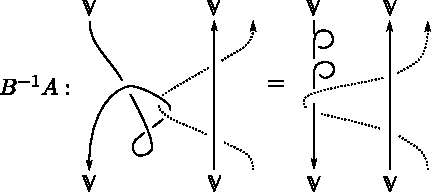
\includegraphics[scale=.8]{../assets/2518/wen_figures/DMoment1.pdf}\nonumber\\
&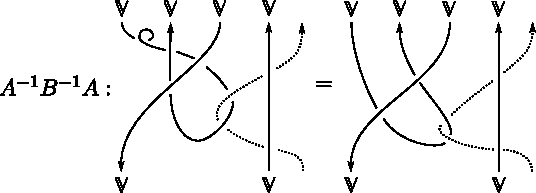
\includegraphics[scale=.8]{../assets/2518/wen_figures/DMoment2.pdf}\nonumber\\
&\begin{array}{c}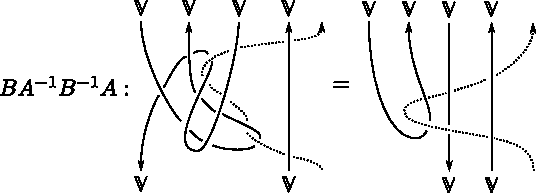
\includegraphics[scale=.8]{../assets/2518/wen_figures/DMoment4.pdf}\end{array}
\label{DMomentDia}
\end{align}
Acting on $V^*\otimes V\subset\OO$, we~obtain
\[
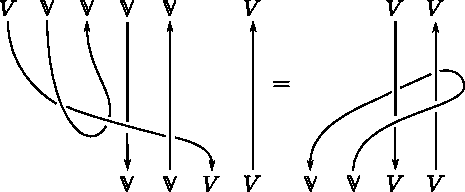
\includegraphics[scale=.8]{../assets/2518/wen_figures/DMoment5.pdf}
\]
upon applying the coend relation \eqref{Coend}.
\end{proof}

\subsubsection{Moment map for $\WW$}\label{WMoment}
The following was proved by Jordan \cite{JordanMult}:

\begin{prop}
The action of the left coideal subalgebra $\kappa(\mathfrak{R})\subset\UU$ on $\WW$ has a quantum moment map
\[
\mu_\WW(m^i_j)= \delta_{i,j}+(1-q^{-2})\del_i\xi_j.
\]
This map is $\UU$-equivariant.
The powers of $\mu_\WW(\det_q(M))$ form an Ore set.
Let $\WWo$ denote the localization at those powers.
Then $\mu_\WW$ extends to a quantum moment map for $\kappa(\OO)$ into $\WWo$.
\end{prop}

Note that the image of $\mu_\WW$ lies in the degree zero part $\WWo_0$.

\begin{prop}\label{WBasic}
We have for $f\in S_q\mathbb{V}$,
\[
\mu_\WW(m^i_j) f=\kappa(m^i_j)\bullet f.
\]
\end{prop}

\begin{proof}
We view $S_q\mathbb{V}$ as the quotient of $\WW$ by the left ideal $I_\del$ generated by $\{ \del_i\}$.
By Proposition \ref{Coideal}, we~have
\[
\mu_\WW(m^i_j)f=\sum_{k}\left(\kappa(m^i_k)\tensor[]{r}{_s} \bullet f\right)\mu_\WW\big(\ad_{\tensor[_s]{r}{}}(m^k_{j})\big).
\]
The equivariance of $\mu_\WW$ implies
\[
\mu_\WW\big(\ad_{\tensor[_s]{r}{}}(m^k_{j})\big)=\tensor[_s]{r}{}\bullet\mu_\WW(m^k_j).
\]
On the other hand, using relations for $\WW$, we~have that after quotienting by $I_\del$,
\[
\mu_\WW(m^k_j) +I_\del=\delta_{k,j}+I_\del.
\]
The proposition follows once we note that $I_\del$ is closed under the $\UU$-action.
\end{proof}

\begin{cor}\label{QDiffMoment}
Recall the map $\mathfrak{qdiff}$ \eqref{QDiffMap}. We~have:
\[
\mathfrak{qdiff}\circ\kappa = \mathfrak{qdiff}\circ\mu_\WW.
\]
\end{cor}

\begin{cor}
The functional representation $S_q\mathbb{V}$ is preserved under the action of the localization $\WWo$.
\end{cor}

\subsubsection{Reduction}\label{Reduct}
Finally, we~consider the tensor product algebra
\[
\MM:=\DD\otimes\WWo
\]
in the braided monoidal category of locally-finite $\UU$-modules.
Thus, the product involves $\mathcal{R}$: for $a_1,a_2\in\DD$ and $b_1,b_2\in\WWo$,
\[
(a_1\otimes b_1)(a_2\otimes b_2)=a_1(\tensor[]{r}{_s}\bowtie a_2)\otimes (\tensor[_s]{r}{}\bullet b_1)b_2.
\]
With this braiding, $\MM$ is a $\UU$-module algebra and thus $\MM^\UU$ is an algebra.

Next, we~collate the moment maps into one for $\MM$. We~define
\[
\mu_{\MM}:=(\mu_\DD\otimes\mu_\WW)\circ(\kappa\otimes\kappa)\circ\nabla:\OO\to\MM.
\]
It is a $\UU$-equivariant algebra homomorphism (each of its components are).
The following is \cite[Prop.\,3.10]{GanJorSaf}, which features a nice diagrammatic proof:

\begin{prop}\label{TensorMoment}
The map $\mu_{\MM}:\OO\to\MM$ is a quantum moment map.
\end{prop}

Recall the determinant character $\chi^k$ defined in \eqref{DetForm}. We~will abuse notation and use $\chi^k$ to also denote the induced character $\chi^k\circ\kappa$ of $\OO$.
In terms of the generating matrix $M$ of $\OO$, we~can use the factorization of $\mathcal{R}$ \eqref{RFactor} to deduce
\[
(1\otimes\chi^k)(M)=q^{-2k}I.
\]

\begin{defn}
Let $\mathcal{I}_k\subset\MM$ be the following left ideal:
\[
\mathcal{I}_k:=\MM\bigl((1\otimes\mu_{\MM})(M)-q^{-2(k-1)}I \bigr).
\]
The \textit{quantized multiplicative quiver variety} is defined to be $\AAA_k:=\big(\MM\big/\mathcal{I}_k\big)^\UU$.
\end{defn}

\begin{prop}[\cite{VarVassRoot,GanJorSaf}]\label{RedAlgProp}
$\AAA_k$ is an algebra.
\end{prop}

\subsubsection{Radial parts map}
Denote by
\[
\left(\OO\otimes S_q\mathbb{V} \right)^{\chi^k}
\]
the subspace where $\UU$ acts by the character $\chi^k$.
From the Peter-Weyl decomposition for $\OO$ \eqref{qPeterWeyl}, we~can see that $q^{\omega_n}$ acts trivially on $\OO$.
Thus,
\[
(\OO\otimes S_q\mathbb{V})^{\chi^k}=(\OO\otimes S_q^{nk}\mathbb{V})^{\chi^k}.
\]
We can further identify
\[
(\OO\otimes S_q^{nk}\mathbb{V})^{\chi^k}\cong (\OO\otimes \rU_k)^\UU=\bigoplus_{\lambda\in P^+}(V_\lambda^*\otimes V_\lambda\otimes \rU_k)^{\UU}.
\]
By Theorem \ref{EtKirMac}, we~can identify the last space with $\Lambda_n^\pm(q)$ by taking the weighted trace.

$\MM$ acts on the tensor product representation $\OO\otimes S_q\mathbb{V}$, where this tensor product representation is taken in the braided monoidal category of locally-finite $\UU$-modules.
Therefore, the action involves the braiding between $\WWo$ and $\OO$ and the action map is $\UU$\nobreakdash-equi\-variant.
This action on $\OO\otimes S_q\mathbb{V}$ then restricts to an action of $\MM^\UU$ on $(\OO\otimes S_q\mathbb{V})^{\chi^k}$.

\begin{prop}\label{AkFact}
For $k\ge 0$, the action of $\MM^\UU$ on $\left(\OO\otimes S_q\mathbb{V} \right)^{\chi^k}$ factors to an action of $\AAA_{k+1}$.
\end{prop}

\begin{proof}
We first show that $\mu_\MM(m^i_j)$ acts on $\OO\otimes S_q\mathbb{V}$ as $\kappa(m^i_j)$ (\ie via the $\UU$-action).
Let $\mathfrak{a}_\MM$ be the action map of $\MM$ on $\OO\otimes S_q\mathbb{V}$.
Using Propositions \ref{DBasic} and \ref{WBasic}, we~have:
\[
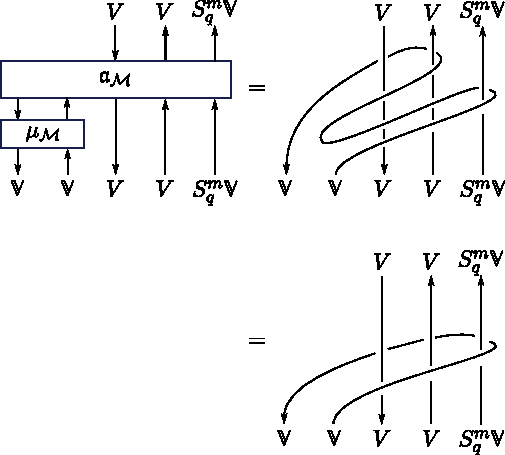
\includegraphics[scale=.8]{../assets/2518/wen_figures/MMoment.pdf}
\]
It follows that the restricted action map
\[
\mathfrak{a}_\MM:\MM\otimes\left(\OO\otimes S_q\mathbb{V} \right)^{\chi^k}\to\OO\otimes S_q\mathbb{V}
\]
factors through $\mathcal{I}_{k+1}$.
The result follows from taking invariants of $\MM\big/\mathcal{I}_{k+1}$.
\end{proof}

\begin{defn}
We denote the representation map by $\mathfrak{rad}_k:\AAA_k\to\mathrm{End}\left(\Lambda_n^\pm(q) \right)$ and called it the \textit{quantum radial parts map}.
\end{defn}

\begin{prop}\label{DAHAContain}
For $k>n$, the image of $\mathfrak{rad}_k$ contains the image of $\SHH_n(q,q^k)$ under $\rrr$:
\[
\mathfrak{rad}_k\left(\AAA_k \right)\supset\rrr\bigl(\SHH_n(q,q^k) \bigr).
\]
Moreover, this inclusion respects the bigradings.
\end{prop}

\begin{proof}
Recall the generators of $\SHH_n(q,q^k)$ from Lemma \ref{GenLem} (in the case $k>n$).
Our analysis in \ref{EtKirDAHA} shows that
\begin{equation}
\begin{aligned}
\mathfrak{rad}_k\bigl(\mathrm{qcoev}_{\wedge_q^r\mathbb{V}}(1) \bigr)&= \rrr\bigl(\ee e_r(\boldsymbol{X}_n)\ee \bigr),\\
\mathfrak{rad}_k\bigl(\partial_\triangleright\mathrm{qcoev}_{\wedge_q^r\mathbb{V}^*}(1) \bigr)&= q^{r(n-1)}\rrr\bigl(\ee e_r(\boldsymbol{Y}^{-1}_n)\ee \bigr),\\
\mathfrak{rad}_k\bigl(\textstyle\det_q(A)^{-1}\bigr)&= \rrr\bigl(\ee \boldsymbol{X}^{-1}_n\ee \bigr),\\
\mathfrak{rad}_k\bigl(\textstyle\det_q(B)\bigr)&= q^{-n(n-1)}\rrr\bigl(\ee \boldsymbol{Y}_n\ee \bigr).
\end{aligned}
\label{RadGen}
\end{equation}
The last two imply the statement about bigradings.
\end{proof}

\section{Isomorphism}

\subsection{Classical degeneration}\label{ClassDegen}
Recall that $\DD_+\subset\DD$ is the subalgebra generated by the entries of $A$ and $B$ (so we exclude those of $A^{-1}$ and $B^{-1}$).
From the relations~\eqref{ABPres} and the formula \eqref{VecRMatrix} for $R$, we~can expect that $\DD_+$ becomes the commutative ring $\CC[\mathfrak{gl}_n\times\mathfrak{gl}_n]$ when $q\mto1$.
Similarly, the quantum Weyl algebra $\WW$ \eqref{WeylPres} should degenerate to the usual Weyl algebra $D(\CC^n)$.
Here, we~review work of Jordan \cite{JordanMult} that makes this precise and we enhance these results to address invariants.

\subsubsection{Lattices}
Let
\[
\MM_+:=\DD_+\otimes\WW
\]
(as in \ref{Reduct}, we~mean the \textit{braided} tensor product of algebras).
As in \cite{JordanMult}, we~define a \textit{standard monomial} in $\MM_+$ to be a product
\begin{equation}
a^{i_1}_{j_1}\cdots a^{i_{\alpha}}_{j_{\alpha}}
b^{k_1}_{\ell_1}\cdots b^{k_{\beta}}_{\ell_{\beta}}
\xi_{r_1}\cdots \xi_{r_\gamma}
\del_{s_1}\cdots\del_{s_\delta},
\label{StandardMon}
\end{equation}
where if $u<v$,
\begin{equation}
\begin{aligned}
&i_u<i_v\hbox{ or }\left(i_u=i_v\hbox{ and }j_u\le j_v\right),\\
&k_u<k_v\hbox{ or }\left(\ell_r=\ell_s\hbox{ and }j_u\le j_v\right),\\
&r_u\le r_v,\\
&s_u\le s_v,
\end{aligned}
\label{StandardIndices}
\end{equation}
whenever such indices are present.

\begin{thm}[\cite{JordanMult}]\label{JorBasis}
Let $\MM_{+,\ZZ}\subset\MM_+$ be the $\CC[q^{\pm 1}]$-subalgebra generated by the generators $\{a^i_j, b^k_\ell, \xi_r, \del_s\}$.
The standard monomials form a basis of $\MM_{+,\ZZ}$.
Thus,
\[
\bigl[ \CC[q^{\pm1}]\big/(q-1) \bigr]\otimes_{\CC[q^{\pm 1}]}\MM_{+,\ZZ}\cong \CC[\mathfrak{gl}_n\times\mathfrak{gl}_n]\otimes D(\CC^n),
\]
where $D(\CC^n)$ is the Weyl algebra.
\end{thm}

For technical reasons, we~will need a slight alteration of this result.
First, we~consider instead the subalgebra $\DD_{\mathrm{IV}}\subset\DD$ generated by the entries of $A$ and $B^{-1}$ and correspondingly set
\[
\MM_{\mathrm{IV}}:=\DD_{\mathrm{IV}}\otimes\WW.
\]
Next, we~will replace $\partial_i$ with
\[
\widetilde{\partial}_i:=(1-q^{-2})\partial_i.
\]
We then define a standard monomial to be
\[
a^{i_1}_{j_1}\cdots a^{i_{\alpha}}_{j_{\alpha}}
\iota(b^{k_{\beta}}_{\ell_{\beta}})\cdots \iota(b^{k_1}_{\ell_1})
\xi_{r_1}\cdots \xi_{r_\gamma}
\widetilde{\del}_{s_1}\cdots\widetilde{\del}_{s_\delta},
\]
where the indices still satisfy \eqref{StandardIndices} when $u<v$.

Let
\[
\mathfrak{M}:=\mathfrak{gl}_n\times\mathfrak{gl_n}\times\CC^n\times\left(\CC^n\right)^*.
\]

\begin{cor}\label{StandardCor}
Let $\MM_{\mathrm{IV},\ZZ}\subset\MM_{\mathrm{IV}}$ be the $\CC[q^{\pm 1}]$-subalgebra generated by
\[
\bigl\{a^i_j, \iota(b^i_j), \xi_r, \widetilde{\del}_s \bigr\}.
\]
The standard monomials form a basis of $\MM_{\mathrm{IV,\ZZ}}$.
Moreover,
\[
\bigl[ \CC[q^{\pm 1}]\big/ (q-1) \bigr]\otimes_{\CC[q^{\pm 1}]}\MM_{\mathrm{IV},\ZZ}\cong \CC[\mathfrak{M}].
\]
\end{cor}

\begin{proof}
The basis statement is clear because $\iota$ is an algebra anti-automorphism---we can map $\MM_+$ isomorphically to $\MM_{\mathrm{IV}}$ within $\DD\otimes\WW$ in a manner that sends standard monomials to standard monomials.
Finally, note that from \eqref{WeylPres}, we~have:
\[
\widetilde{\partial}_i\xi_i= (1-q^{-2})+q^2\xi_i\widetilde{\partial}_i+(q^2-1)\sum_{k>i}\xi_k\widetilde{\partial}_k.
\]
Therefore, $\left[ \CC[q^{\pm 1}]\big/(q-1) \right]\otimes_{\CC[q^{\pm 1}]}\MM_{\mathrm{IV},\ZZ}$ is a commutative ring.
\end{proof}

Thus, whenever we perform $q\mto 1$ degeneration in $\mathcal{M}_{\mathrm{IV}}$, it will always be with respect to this basis of standard monomials.
Namely, for any subspace $V\subset\MM_{\mathrm{IV}}$, we~define:
\begin{align}
V_\ZZ&:= V\cap \MM_{\mathrm{IV},\ZZ},\\
V_{q=1}&:=\Bigl\{f_1(1)M_1+\cdots +f_m(1)M_m\Bigm|
\begin{array}{l}
f_1(q)M_1+\cdots+f_m(q)M_m\in V_\ZZ\hbox{ for}\\
\hbox{standard monomials }M_1,\ldots ,M_m
\end{array}
\Bigr\}.
\label{DegenDef}
\end{align}

\begin{prop}\label{DimProp}
For a finite-dimensional subspace $V\subset\MM_{\mathrm{IV}}$, we~have:
\begin{equation}
\dim_{\CC(q)}V= \mathrm{rank}_{\CC[q^{\pm 1}]}V_\ZZ =\dim_{\CC}V_{q=1}.
\label{DimBound}
\end{equation}
\end{prop}

\begin{proof}
This follows from the fact that $\MM_{\mathrm{IV,\ZZ}}$ is free and $\CC[q^{\pm 1}]$ is a PID.
\end{proof}

\subsubsection{Invariants}
We endow $\CC[\mathfrak{M}]=\CC\left[\mathfrak{gl}_n\times\mathfrak{gl}_n\times\CC^n\times\left(\CC^n\right)^*\right]$ with the following $\GL_n$-action:
for the natural coordinate functions $(X,Y,i,j)$ on $\mathfrak{M}$ and $g\in \GL_n$, let
\[
g(X,Y,i,j)=(g^{-1}Xg, g^{-1}Yg, (g^{-1})i, jg).
\]
Here, we~view the last factor $j$ as a row vector.
$U(\mathfrak{gl}_n)$ then acts on $\CC[\mathfrak{M}]$ via derivations induced by the coadjoint and vector representations.
By a classic theorem of Weyl \cite{WeylInv}, $\CC[\mathfrak{M}]^{\GL_n}$ is generated by \textit{classical trace functions}:
\begin{equation}
\tr(X^{a_1}Y^{b_1}(i j)^{c_1}\cdots X^{a_m}Y^{b_m}(i j)^{c_m})
\label{ClassTrace}
\end{equation}
for $a_1,b_1,c_1, a_2,b_2, c_2,\ldots, a_m,b_m, c_m\in\ZZ_{\ge 0}$.

We identify $(A,B^{-1},(1-q^{-2})\vec{\partial},\vec{\xi})$ with $(X,Y,i,j)$ in the $q\mto 1$ degeneration as follows:
\begin{equation}
A\mto X,\quad B^{-1}\mto Y,\quad (1-q^{-2})\vec{\partial}\mto i,\quad \vec{\xi}\mto j.
\label{DegenTrans}
\end{equation}
With this, let us define natural quantum versions of \eqref{ClassTrace}.
For $k\ge 0$, we~define the \textit{quantum trace} of $M^k$ as:
\begin{equation}
\tr_q(M^k):=\sum_{1\le i_1,\ldots, i_k\le n} q^{-\langle 2\rho,\epsilon_{i_k}\rangle} m^{i_k}_{i_1}m^{i_1}_{i_2}\cdots m^{i_{k-1}}_{i_{k}}.
\label{QTraceM}
\end{equation}
Similarly, for $a_1,b_1,c_1, a_2,b_2, c_2,\ldots, a_m,b_m, c_m\in\ZZ_{\ge 0}$, we~define
\begin{equation}
\tr_q\left(A^{a_1}B^{-b_1}(\mu_{\WW}(M)-I)^{c_1}\cdots A^{a_m}B^{-b_m}(\mu_{\WW}(M)-I)^{c_m}\right)\in\MM_{\mathrm{IV}}
\label{QTrace}
\end{equation}
as \eqref{QTraceM} with $m_{j}^i$ replaced with $a^{i}_j$, $\iota(b)^{i}_j$, or
\[
\left(\mu_{\WW}(M)-I \right)^i_j=\widetilde{\partial}_i\xi_j,
\]
depending on the location. We~call these \textit{quantum trace elements}.

\begin{prop}\label{QTraceProp}
The quantum traces are elements of $\MM_{\mathrm{IV}}^\UU\cap\MM_{\mathrm{IV,\ZZ}}$ that are sent to their corresponding classical traces when $q\mto 1$.
\end{prop}

\begin{proof}
It is obvious that quantum traces are contained in $\MM_{\mathrm{IV},\ZZ}$ and are sent to~\eqref{ClassTrace} when $q\mto 1$.
To see that they are $\UU$-invariants, observe that they are the image of~$1\in\mathbbm{1}$ under a composition of $\UU$-morphisms:
\begin{enumerate}
\item the map $\mathbbm{1}\to (\mathbb{V}^*\otimes\mathbb{V})^{\otimes k}$ induced by
\[
1\mto \sum_{1\le i_1,\ldots, i_k\le n} q^{-\langle 2\rho,\epsilon_{i_k}\rangle} m^{i_k}_{i_1}\otimes m^{i_1}_{i_2}\otimes \cdots\otimes m^{i_{k-1}}_{i_{k}},
\]
which is depicted diagrammatically as
\[
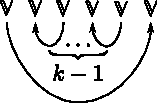
\includegraphics[scale=.8]{../assets/2518/wen_figures/Wilson.pdf}
\]
\item the antipode $\iota$ on tensorands that will correspond to $B^{-1}$ matrix elements;
\item the inclusion into $\MM_{\mathrm{IV}}$ (identity for $A$-matrix elements, $\partial_\triangleright$ for $B^{-1}$-matrix elements, and $\mu_W-\mathrm{ev}_{\mathbb{V}}$);
\item the product in $\MM_{\mathrm{IV}}$.\qedhere
\end{enumerate}
\end{proof}

\begin{lem}\label{InvLem}
For any $\UU$-submodule $V\subset\MM_{\mathrm{IV}}$, $V_{q=1}$ is a $\GL_n$-module.
Furthermore, we~have
\[
[ V^\UU]_{q=1}=[ V_{q=1}]^{\GL_n}.
\]
\end{lem}

\begin{proof}
Observe that $\UU$ acts on standard monomials in a way that preserves the lattice $\MM_{\mathrm{IV},\ZZ}$.
Moreover, because of \eqref{DegenTrans}, the action of $E_i$ and $F_i$ degenerate to the action of their corresponding generators $e_i,f_i\in U(\mathfrak{gl}_n)$ on monomials in $\CC[\mathfrak{M}]$.
Finally, the degeneration preserves the weight.
Thus, $V_{q=1}$ is a $\GL_n$-module and we have the containment
\[
[ V^\UU]_{q=1}\subset[ V_{q=1}]^{\GL_n}.
\]

For the other containment, let $v\in V_\ZZ$ be a lift of $\mathfrak{v}\in \left[ V_{q=1} \right]^{\GL_n}$. We~can write $\mathfrak{v}$ in terms of classical traces.
Let $\tr_q^\mathfrak{v}\in\MM_{\mathrm{IV},\ZZ}$ be the element where every classical trace is replaced with its quantum version. We~can write
\[
v=\tr_q^\mathfrak{v}+(q-1)w
\]
for some $w\in\MM_{\mathrm{IV,\ZZ}}$.
Since $\tr_q^{\mathfrak{v}}$ is $\UU$-invariant, we~have that
\[
E_iv=(q-1)E_iw,\quad F_iv= (q-1)F_i w
\]
for all $i$.
If $v\not\in V^\UU$, then one of the expressions above is nonzero and $w\in V$ due to complete reducibility ($\MM_{\mathrm{IV}}$ is locally-finite).
It then follows that $\tr_q^{\mathfrak{v}}$ is an element of $V^\UU\cap\MM_{\mathrm{IV},\ZZ}$ that lifts $\mathfrak{v}$.
\end{proof}

We can combine \eqref{DimBound} with Lemma \ref{InvLem} to obtain:
\begin{prop}\label{DInvProp}
For a finite-dimensional $\UU$-submodule $V\subset\MM_{\mathrm{IV}}$,
\begin{equation}
\dim_{\CC(q)} V^\UU = \dim_\CC[ V_{q=1}]^{\GL_n}.
\label{InvBound}
\end{equation}
\end{prop}

\subsection{The case $t=q^k$}\label{qkCase}
By Proposition \ref{DAHAContain}, $\AAA_k$ is at least as large as $\SHH_n(q,q^k)$.
Our strategy to handle the $t=q^k$ case is to show that $\AAA_k$ is also no bigger than $\SHH_n(q,q^k)$.
Of course, this is but an impressionistic statement---we will need to make it precise.

\subsubsection{Mise en place}
We begin with a little result that allows us to focus on $\DD$:

\begin{lem}\label{DGenerate}
The image of the composition
\[
\DD^\UU\hto\MM^\UU\to\AAA_k
\]
becomes all of $\AAA_k$ after performing a localization.
\end{lem}

\begin{proof}
First note that by considering the action of $q^{\omega_n}$, any $\UU$-invariant of $\MM$ must have degree zero in its $\WW$ component, \ie
\begin{align*}
\MM^\UU&=\left(\DD\otimes\WW_0^\circ \right)^\UU,\\
\mathcal{I}_k^\UU&= \left(\mathcal{I}_k\cap\DD\otimes\WW_0^\circ \right)^\UU.
\end{align*}
From multiplication \textit{on the left}, we~have
\begin{equation}
\DD\otimes\WW_0\Bigl(\delta_{i,j}+(q-q^{-1})\del_i\xi_j -q^{-2k}\sum_i(A^{-1}BAB^{-1})_j^i\Bigr)\subset\mathcal{I}_k\cap\DD\otimes\WW_0.
\label{MomentDGenerate}
\end{equation}
On the other hand, $\WW_0$ is generated by $\{\del_i\xi_j\}$.
For any $w\in\WW_0$ and $x\in\DD$, we~can use the R-matrix to move $w$ to the right:
\[
wx=(\tensor[]{r}{_s}\bowtie x)(\tensor[_s]{r}{}\bullet w).
\]
We can then use \eqref{MomentDGenerate} to write $\tensor[_s]{r}{}\bullet w$ in terms of $\DD$ in the quotient
\[
\DD\otimes\WW_0\big/(\mathcal{I}_k\cap\DD\otimes\WW_0).
\]
Therefore, the map
\[
\DD\hto\DD\otimes\WW_0\to\DD\otimes\WW_0\big/(\mathcal{I}_k\cap\DD\otimes\WW_0)
\]
is surjective.
Since all the $\UU$-modules involved are locally-finite, taking $\UU$-invariants is exact.
After doing so, $\det_q(M)$ can be written in terms of elements of $\DD^\UU$. We~localize the image at that latter expression.
\end{proof}

\begin{cor}\label{ALocCor}
$\AAA_k$ is a localization of $\AAA_{k,\mathrm{IV}}:=\DD_{\mathrm{IV}}^\UU\big/(\DD_{\mathrm{IV}}\cap\mathcal{I}_k)^\UU$.
\end{cor}

We can thus focus on $\mathcal{D}_{\mathrm{IV}}$ and $\AAA_{k,\mathrm{IV}}$.
The left ideal $\mathcal{I}_k$ is generated by elements with homogeneous determinant bigrading, and so $\AAA_k$ and $\AAA_{k,\mathrm{IV}}$ are also bigraded.
Let $\AAA_{k,\mathrm{IV}}[a,b]$ denote its bidegree $(a,b)$ piece.
Recall our notation from Section~\ref{DAHABigrad}.
Proposition \ref{DAHAContain} implies that
\begin{equation}
\dim_{\CC(q)}\AAA_{k,\mathrm{IV}}[a,-b]\ge\dim_{\CC(q)}\mathcal{S}_{q^k,\mathrm{IV}}[a,-b]=\dim_\CC\CC\left[ \boldsymbol{x}_n,\boldsymbol{y}_n \right]^{\Sigma_n}_{a,b}.
\label{ABig}
\end{equation}
We will use classical degeneration, as covered in \ref{ClassDegen}, to obtain the opposite bound.

\subsubsection{Almost commuting variety}
Let $\mathfrak{M}_{\mathrm{ac}}\subset\mathfrak{M}=\CC\bigl[\mathfrak{gl}_n\times\mathfrak{gl}_n\times\CC^n\times(\CC^n)^*\bigr]$ be the closed subscheme with ideal generated by the entries of
\begin{equation}
[X,Y]-ij,
\label{ACEquation}
\end{equation}
where $(X,Y,i,j)$ are the usual coordinates of $\mathfrak{M}$.
The following results are proved by Gan--Ginzburg \cite{GanGinz}:
\begin{thm}
The projection map $p:\mathfrak{M}\to\mathfrak{gl}_n\times\mathfrak{gl_n}$ induces an isomorphism:
\begin{equation}
\CC[\mathfrak{M}_{\mathrm{ac}}]^{\GL_n}\cong\bigl(\CC[\mathfrak{gl}_n\times\mathfrak{gl}_n]\big/I\bigr)^{\GL_n}
\cong \CC[\boldsymbol{x}_n,\boldsymbol{y}_n]^{\Sigma_n},
\label{ACIso}
\end{equation}
where $I$ is the ideal generated by the equations $[X,Y]=0$ and the second isomorphism is induced by restriction to diagonal matrices.
\end{thm}

$\mathfrak{M}_{\textrm{ac}}$ is called the \textit{almost commuting variety}.
We can endow $\CC[\mathfrak{M}]$ with a bigrading where the entries of $X$ have bidegree $(1,0)$ and those of $Y$ have bidegree $(0,1)$.
The ideal \eqref{ACEquation} identifies elements of bidegree $(1,1)$ with those of bidegree $(0,0)$, so $\CC[\MM_{\mathrm{ac}}]$ inherits this bigrading.
Let $\CC\langle X,Y\rangle\subset\CC[\mathfrak{M}_{\mathrm{ac}}]$ denote the subalgebra generated by the entries of $X$ and $Y$ and let $\CC\langle X,Y\rangle^{\GL_n}_{a,b}$ denote the bidegree $(a,b)$ piece of the invariant subalgebra.
Tracing through the isomorphism \eqref{ACIso}, we~have:
\begin{cor}\label{ACCor}
For each bidegree $(a,b)$,
\[
\dim_\CC\CC\langle X,Y\rangle_{a,b}^{\GL_n}=\dim_\CC\CC[\boldsymbol{x}_n,\boldsymbol{y}_n]^{\Sigma_n}_{a,b}.
\]
\end{cor}

\begin{lem}\label{ACLem}
There is an algebra homomorphism
\[
\psi:\CC[\mathfrak{M}_{\mathrm{ac}}]\to\left(\MM_{\mathrm{IV}}\right)_{q=1}\big/\left(\mathcal{I}_k\cap\MM_{\mathrm{IV}}\right)_{q=1}
\]
that restricts to a surjection
\[
\psi:\CC\langle X,Y\rangle\onto\left(\DD_{\mathrm{IV}} \right)_{q=1}\big/\left(\mathcal{I}_k\cap\DD_{\mathrm{IV}}\right)_{q=1}
\]
which respects bigradings.
\end{lem}

\begin{proof}
From \textit{left} multiplication on the generators of $\mathcal{I}_k$, we~can see that
\begin{equation}
\MM_{\mathrm{IV}}\big((B^{-1}A)^i_j+(B^{-1}A)^i_\ell\widetilde{\partial}_{\ell}\xi_j-q^{-2k}(AB^{-1})^i_j\big)\subset\mathcal{I}_k\cap\MM_{\mathrm{IV}}.
\label{ACContain}
\end{equation}
Let $(A,B^{-1},\vec{\xi},\vec{\partial})$ denote the coordinates of $\mathrm{Spec}\left(\MM_{\mathrm{IV}}\right)_{q=1}\cong\mathfrak{M}$ and $(X,Y, i, j)$ denote the coordinates for another copy of $\mathfrak{M}$.
Upon setting $q=1$, the containments \eqref{ACContain} imply that
\[
\left(X,Y,i, j\right)\mto(A, B^{-1}, B^{-1}A\vec{\partial},\vec{\xi},)
\]
induces the desired homomorphism $\psi$.
\end{proof}

\begin{thm}\label{qkCaseThm}
For $k>n$, the radial parts map $\mathfrak{rad}_k$ gives an isomorphism
\[
\AAA_k\cong\SHH_n(q,q^k).
\]
\end{thm}

\begin{proof}
By Lemma \ref{GenLem}, equations \eqref{RadGen}, and Corollary \ref{ALocCor}, it suffices to show that $\mathfrak{rad}_k$ restricts to an isomorphism
\[
\AAA_{k,\mathrm{IV}}\cong\SHH_n(q,q^k)_{\mathrm{IV}},
\]
because localization is exact.
To that end, we~just need to provide the opposite bound to \eqref{ABig}.
Applying Propositions \ref{DimProp} and \ref{DInvProp} and Lemma \ref{InvLem}, we~have
\begin{align}
\dim_{\CC(q)}\AAA_{k,\mathrm{IV}}[a,b]&=\dim_{\CC(q)}\DD_{\mathrm{IV}}^\UU[a,b]-\dim_{\CC(q)}\mathcal{I}_k\cap\DD_{\mathrm{IV}}^\UU[a,b]\nonumber\\
&= \dim_{\CC}\left(\DD_{\mathrm{IV}}[a,b]_{q=1} \right)^{\GL_n}-\dim_{\CC}\left(\mathcal{I}_k\cap\DD_{\mathrm{IV}}[a,b]_{q=1}\right)^{\GL_n}\nonumber\\
&= \dim_{\CC}\bigl[ \left(\DD_{\mathrm{IV}}\right)_{q=1}\big/(\mathcal{I}_k\cap\DD_{\mathrm{IV}})_{q=1} \bigr]^{\GL_n}_{a,b},\label{qklastinequal}
\end{align}
where in the final line, the subscript denotes the bidegree $(a,b)$ piece.
Finally, we~can combine Corollary \ref{ACCor} and Lemma \ref{ACLem} to bound \eqref{qklastinequal} above by $\dim_\CC\CC[\boldsymbol{x}_n,\boldsymbol{y}_n]_{a,b}^{\Sigma_n}$.
\end{proof}

\subsection{Generic parameters}\label{GenPar}
Now we introduce the variable $t$ and establish the isomorphism over $K=\CC(q,t)$.
Let $\UU_t:=K\otimes\UU$. We~will base change $\UU$ and all its modules to $\UU_t$ but still denote them by the same symbols to avoid notational clutter.
Let $\alpha$ be a parameter such that $t=q^\alpha$; we introduce it for stylistic/notational reasons so as to neatly replace the integer $k$.
All constructions below can be described fully in terms of $t$ rather than $\alpha$.

\subsubsection{Etingof--Kirillov theory at $t$}
In order to extend \ref{EtKirThy}, we~need a suitable generalization of $S_q^{nk}\mathbb{V}$, and moreover it should be a representation of $\WWo_0$.
Recall the notation from \ref{WeylDiff}, wherein we translated the actions of $\UU$ and $\WW$ on $S_q\mathbb{V}$ to ones on the polynomial ring $\CC(q)[\boldsymbol{z}_n]:=\CC(q)[z_1,\ldots,z_n]$.
From this we constructed an algebra homomorphism
\[
\mathfrak{qdiff}:\WW\rtimes\UU\to\mathbb{D}_q(\boldsymbol{z}_n),
\]
where $\mathbb{D}_q(\boldsymbol{z}_n)$ is a ring of difference operators.
Using Corollary \ref{QDiffMoment} and the $\UU$\nobreakdash-equi\-variance of $\mu_\WW$, we~can extend $\mathfrak{qdiff}$ to $\WWo\rtimes\UU$ by setting
\[
\mathfrak{qdiff}(\mu_\MM(\textstyle\det_q(M))^{-1})=(\mathfrak{qdiff}\circ\kappa)(\textstyle\det_q(M)^{-1})=\mathfrak{qdiff}(q^{2\omega_n}).
\]
We will abuse notation and use $\mathfrak{qdiff}$ to also denote its base change to $K$.

Let $W_\alpha$ be the $K$-vector space spanned by ``monomials'' of the form
\[
\bigl\{z_1^{k_1+\alpha-1}z_2^{k_2+\alpha-1}\cdots z_n^{k_n+\alpha-1}\bigm| (k_1,\ldots, k_n)\in\ZZ^n \bigr\}.
\]
We emphasize that the $k_i$ are now allowed to be negative.
$\mathbb{D}_q(\boldsymbol{z}_n)$ naturally acts on this space by
\begin{align*}
z_i\bigl(z_1^{k_1+\alpha-1}\cdots z_n^{k_n+\alpha-1}\bigr)&= z_1^{k_1+\alpha-1}\cdots z_i^{k_i+1+\alpha-1}\cdots z_n^{k_n+\alpha-1},\\
T_{q,z_i} \bigl(z_1^{k_1+\alpha-1}\cdots z_n^{k_n+\alpha-1}\bigr)&= q^{k_i-1}tz_1^{k_1+\alpha-1}\cdots z_n^{k_n+\alpha-1}.
\end{align*}
Therefore, we~obtain an action of $\WWo\rtimes\UU_t$ on $W_\alpha$.
In particular, the $\WWo$-action is $\UU_t$-equivariant.
From the formulas \eqref{QDiffMap} for $\mathfrak{qdiff}$, it is clear that $\WWo_0\rtimes\UU$ preserves the subspace
\[
W^0_\alpha:=
\mathrm{span}_{K}\Bigl\{z_1^{k_1+\alpha-1}z_2^{k_2+\alpha-1}\cdots z_n^{k_n+\alpha-1}\Bigm|
\begin{array}{l}
(k_1,\ldots, k_n)\in\ZZ^n \\
k_1+\cdots +k_n=0
\end{array}
\Bigr\}.
\]
$W^0_\alpha$ will be our replacement for $S_q^{n(k-1)}\mathbb{V}$.

Next, we~will need a $t$-version of the determinant representation.
Let $\chi^{\pm\alpha}:\UU_t\to K$ be the characters given by
\begin{equation*}
\chi(E_i)=\chi(F_i)=0,\quad
\chi(q^{h})=t^{\pm\langle h,\omega_n\rangle}.
\end{equation*}
We denote by $\mathbbm{1}_{-\alpha}\cong K$ the dimension 1 representation defined using $\chi^{-\alpha}$.
It is natural to interpret integer shifts of $\alpha$ as tensoring by $\mathbbm{1}_k$.
The zero weight space $W_\alpha\otimes\mathbbm{1}_{1-\alpha}[0]$ is of dimension 1, spanned by $z_1^{\alpha-1}\cdots z_n^{\alpha-1}\otimes 1$; we thus identify it with $K$.

Finally, $V_{\lambda+(k-1)\delta}$ is replaced with the \textit{Verma} module
\[
M_\lambda^\alpha:=M_{\lambda+(\alpha-1)\delta},
\]
which is simple when $t$ is left as a parameter.
With this set, the case of general $t$ is in many ways quite similar to that of $t=q^k$.
\begin{thm}[\cite{EtKirQuant}]
We have the following:
\begin{enumerate}
\item For $\lambda\in P$, there is a nonzero, unique up to constant intertwiner
\[
\widetilde{\Phi}_\lambda^\alpha: M_{\lambda}^{\alpha}\to M_{\lambda}^{\alpha}\otimes W^0_{\alpha}\otimes\mathbbm{1}_{1-\alpha}.
\]
\item For $\lambda\in P^+$, upon picking consistent normalizations for $\{ \widetilde{\Phi}_\lambda^\alpha \}$, the weighted trace $\widetilde{\varphi}^\alpha_{\lambda}$ satisfies
\[
P_\lambda(q,t)=\widetilde{\varphi}_{\lambda}^\alpha\big/\widetilde{\varphi}_{0}^\alpha.
\]
\end{enumerate}
\end{thm}
We note in passing that $\widetilde{\varphi}_{\lambda}^\alpha$ is no longer a polynomial but rather a power series.

\subsubsection{Admissible diagrams}\label{Diagrams}
Since $M_{\lambda}^\alpha$ is infinite-dimensional, we~can no longer convert the intertwiner $\widetilde{\Phi}^\alpha_{\lambda}$ into an invariant vector as we we did in \ref{EtKirThy}.
More generally, the graphical calculus covered in \ref{Reps} still applies to $M_\lambda$ except that it no longer has classical and quantum coevaluations.
This leads to some awkwardness in defining the action of non-invariant elements of $\MM$.
Our goal here is to be able to turn elements of $\MM$ ``upside-down''.

We have already made use of diagrammatic calculus for $\DD$---let us give a similar construction for $\WWo$.
The inclusion of the generators $\{\partial_i\}$ and $\{\xi_i\}$ come from morphisms $\mathbb{V}^*\to\WW$ and $\mathbb{V}\to\WW$, respectively, and likewise the inclusion of $\mu_\MM(\det_q(M))^{-1}$ comes from a morphism $\mathbbm{1}\to\WWo$.
Since the product $\mathfrak{m}_\WW$ of $\WWo$ is a $\UU$-morphism, we~can write any element of $\WWo$ as a linear combination of images of morphisms $\mathfrak{d}:X\to\WWo$ for some $\UU$-module $X$.

Altogether, we~have a way to present elements of $\MM\cong\OO\otimes\kappa(\OO)\otimes\WWo$ as a linear combination of morphisms of the form
\begin{equation}
\begin{array}{c}
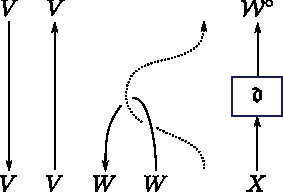
\includegraphics[scale=.8]{../assets/2518/wen_figures/DAB.pdf}
\end{array}
\label{DAB}
\end{equation}
evaluated at various inputs. We~can define a product $*$ of two such morphisms by
\[
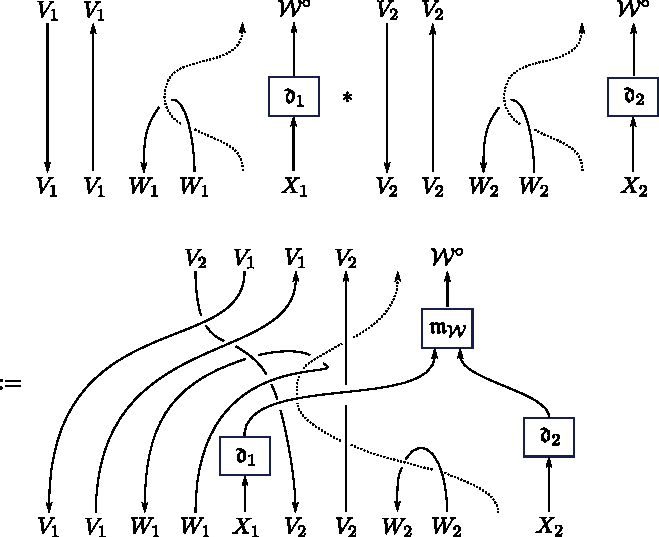
\includegraphics[scale=.8]{../assets/2518/wen_figures/StarProd.pdf}
\]
This yields the product in $\MM$ upon evaluation.

More generally, the diagram of a morphism $\mathfrak{D}:W_1\otimes W_2\to\MM$ is called \textit{admissible} if it is of the form
\begin{equation}
\begin{array}{c}
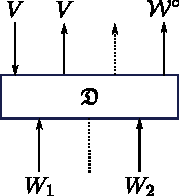
\includegraphics[scale=.8]{../assets/2518/wen_figures/D1.pdf}
\end{array}
\label{Admiss}
\end{equation}
where the ghost strand only undergoes braidings.
For such a $\mathfrak{D}$, we~define
\[
\overline{\mathfrak{D}}:\OO\to\WWo\otimes W_2^*\otimes\UU\otimes W_1^*
\]
to be the morphism given by
\[
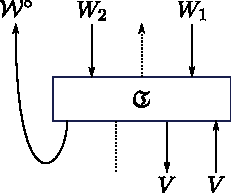
\includegraphics[scale=.8]{../assets/2518/wen_figures/DBar.pdf}
\]
where every morphism inside $\mathfrak{D}$ is replaced with its adjoint and the orientation of the ghost strand is reversed.
While $\WWo$ is infinite-dimensional, it is locally finite and thus the coevaluation is done on a finite-dimensional subrepresentation.
Specializing $\UU$ to act on a finite-dimensional module $U$, $\overline{\mathfrak{D}}$ is obtained from $\mathfrak{D}$ in terms of partial adjoints.
Thus, this is an operation on morphisms, not just diagrams.

Finally, for a diagram $\mathfrak{D}_1$ like \eqref{DAB} and a general admissible diagram $\mathfrak{D}_2$, we~define the product $\mathfrak{D}_1*\mathfrak{D}_2$ by:
\[
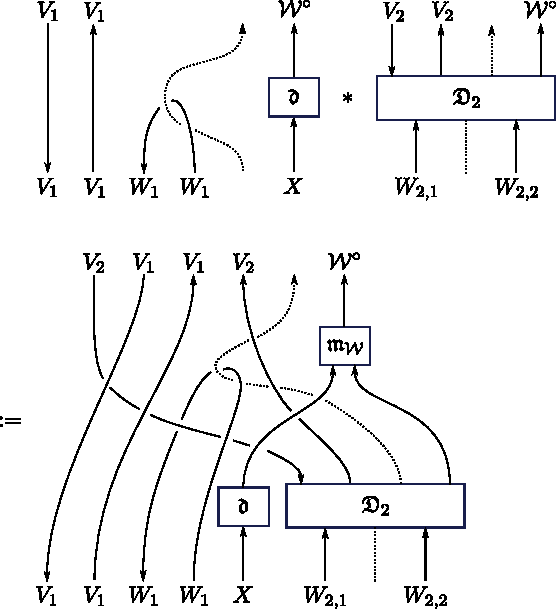
\includegraphics[scale=.8]{../assets/2518/wen_figures/StarProd2.pdf}
\]
Observe that $\mathfrak{D}_1*\mathfrak{D}_2$ is also admissible.

\subsubsection{Action on linear maps}
Let
\begin{multline}
\mathfrak{tHom}_\alpha
:=
\bigoplus_{\substack{M\text{ highest weight}\\ U\text{ finite-dimensional}}}
\Hom_\UU\left(M, M\otimes W_{\alpha}\otimes U^*\right) \Big/\\
\Bigl\langle
(f\otimes 1\otimes 1)\circ \psi -\psi \circ f\Bigm|
\begin{array}{l}
\psi\in\Hom_\UU\left(M', M\otimes W_{\alpha}\otimes U^*\right),\\
f\in\Hom_\UU(M,M')
\end{array}
\Bigr\rangle.
\label{tHomRel}
\end{multline}
The relations \eqref{tHomRel} are analogous to the coend relations \eqref{Coend}---the ``t'' stands for homomorphisms identified if they have the same trace.
One should view the extra tensorand $U^*$ as something we will contract away to yield an $K$-linear map $M\to M\otimes W_{\alpha}$.
Since the Verma module $M_{\lambda}^{\alpha}$ is simple, the intertwiners $\{\widetilde{\Phi}_\lambda^\alpha\}$ are linearly independent in $\mathfrak{tHom}_\alpha$.

Let $\mathfrak{a}_\WW:\WWo\otimes W_\alpha\to W_\alpha$ be the action map.
For an admissible diagram $\mathfrak{D}:W_1\otimes W_2\to \MM$ as in \eqref{Admiss} and
\[
\phi\in\Hom_\UU\left(M, M\otimes W_{\alpha}\otimes U^*\right)\subset\mathfrak{tHom}_\alpha,
\]
we define
\[
\mathfrak{D}\star\phi: V\otimes M\to (V\otimes M)\otimes W_{\alpha} \otimes (W_1\otimes W_2\otimes U)^*
\]
to be the class of the morphism:
\begin{equation}
\begin{array}{c}
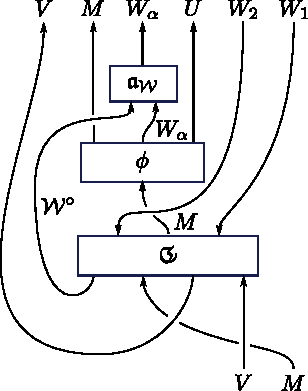
\includegraphics[scale=.8]{../assets/2518/wen_figures/DiaAct.pdf}
\end{array}
\label{DiaAct}
\end{equation}
Such a morphism is well-defined for infinite-dimensional $M$ because $M$ only undergoes braidings.
Moreover, any $f$ as in the relations \eqref{tHomRel} can pass through such braidings.
This implies that $\mathfrak{D}\star\phi$ is independent of the representative of the class of $\phi$. We~leave it as a drawing exercise to see that for a diagram $\mathfrak{D}_1$ of the form \eqref{DAB} and an admissible diagram $\mathfrak{D}_2$, we~have
\begin{equation}
\mathfrak{D}_1\star\left(\mathfrak{D}_2\star\phi \right)=\left(\mathfrak{D}_1*\mathfrak{D}_2 \right)\star\phi.
\label{MProdAct}
\end{equation}

Consider now the space of $K$-linear maps:
\begin{multline}
\mathrm{tHom}_\alpha:=\bigoplus_{M\text{ is highest weight}}\Hom_{R_q}\left(M, M\otimes W_{\alpha}\otimes\mathbbm{1}_{1-\alpha}\right)\Big/\\
\Bigl\langle
(f\otimes 1)\circ \psi -\psi \circ f\Bigm|
\begin{array}{l}
\psi\in\Hom_{R_q}\left(M', M\otimes W_{\alpha}\otimes\mathbbm{1}_{1-\alpha}\right),\\
f\in\Hom_\UU(M,M')
\end{array}
\Bigr\rangle.
\label{tHomLinRel}
\end{multline}
For the class of $\phi:M\to M\otimes W_{\alpha}\otimes\mathbbm{1}_{1-\alpha}$ in $\mathrm{tHom}_\alpha$, we~define an operation by each of the three tensor components of $\MM\cong\OO\otimes\partial_{\triangleright}(\OO)\otimes \WWo$:
\begin{itemize}
\item for $v^*\otimes v\in V^*\otimes V\subset\OO\otimes1\subset\DD$, define
\begin{equation}
\begin{gathered}
(v^*\otimes v)\star\phi:V\otimes M\to V\otimes M\otimes W_{\alpha}\otimes\mathbbm{1}_{1-\alpha}\\
\big((v^*\otimes v)\star\phi\big)(x\otimes m)=v^*(\tensor[_s]{r}{}x)\bigl[S(\tensor[_t]{r}{})v\otimes\phi(\tensor[]{r}{_t}\tensor[]{r}{_s}m)\bigr];
\end{gathered}
\label{tHomActA}
\end{equation}
\item for $\kappa(v^*\otimes v)\in 1\otimes\partial_{\triangleright}(\OO)\subset\DD$, define
\begin{equation}
\begin{gathered}
\kappa(v^*\otimes v)\star\phi:M\to M\otimes W_{\alpha}\otimes\mathbbm{1}_{1-\alpha}\\
\big(\kappa(v^*\otimes v)\star\phi\big)(m)=v^*\left(S(\tensor[_t]{r}{}\tensor[]{r}{_s})v\right)\phi(\tensor[]{r}{_t}\tensor[_s]{r}{}m);
\end{gathered}
\label{tHomActB}
\end{equation}
\item for $w\in \WWo$ define
\begin{equation}
\begin{gathered}
w\star\phi:M\to M\otimes W_{\alpha}\otimes\mathbbm{1}_{1-\alpha}\\
\big(w\star\phi\big)(m)=\left(\tensor[]{r}{_t}\otimes (\tensor[_t]{r}{}S(\tensor[_s]{r}{})\bullet w) \otimes 1\right)\blacktriangleright\phi(\tensor[]{r}{_s}m),
\end{gathered}
\label{tHomActW}
\end{equation}
where the $\blacktriangleright$ means acting on the output of $\phi$ via the $\UU$- and $\WWo$-actions.
\end{itemize}
Because the input of $\phi$ and $M$-tensorand of the output of $\phi$ is only acted on by elements of $\UU$, these operations are well-defined on the quotient \eqref{tHomLinRel}.
{A priori}, we~do not know that they piece together to form an action of $\MM$.
To that end, let:
\begin{itemize}
\item $\mathrm{tHom}_\alpha^{D}$ be the subspace of $\mathrm{tHom}_\alpha$ generated by these operations from the intertwiners $\{ \widetilde{\Phi}_{\lambda}^\alpha \}_{\lambda\in P}$ (the $D$ is for ``diagram'');
\item $\mathrm{Int}_\alpha\subset\mathrm{tHom}_\alpha^{D}$ be the span of $\{ \widetilde{\Phi}_{\lambda}^\alpha \}_{\lambda\in P}$;
\item $\mathrm{Int}_\alpha^+\subset\mathrm{Int}_\alpha$ be the span of $\{\widetilde{\Phi}_\lambda^\alpha\}_{\lambda\in P^+}$.
\end{itemize}
Finally, we~set
\begin{align*}
\MM_{[t]}&:= \CC(q)[t^{\pm 1}] \otimes\MM,\\
\MM_K&:= K\otimes\MM=\CC(q,t)\otimes\MM.
\end{align*}

\begin{lem}
The operations \eqref{tHomActA}--\eqref{tHomActW} define actions of $\MM_{[t]}$ and $\MM_K$ on $\mathrm{tHom}_\alpha^D$.
Under this action, $\MM^\UU$ preserves $\mathrm{Int}_\alpha$.
\end{lem}

\begin{rem}
The formulas \eqref{tHomActA}--\eqref{tHomActW} should define an action of $\MM$ on the entire space $\mathrm{tHom}_\alpha$. We~leave the proof to a more skillful scholar of the Yang-Baxter equation.
\end{rem}

\begin{proof}
On $\mathrm{tHom}_\alpha^D$, the operations \eqref{tHomActA}--\eqref{tHomActW} are obtained by contracting the diagram actions on $\mathfrak{tHom}_\alpha$ with $\phi$ set equal to an intertwiner $\widetilde{\Phi}_\lambda^\alpha$.
Equation \eqref{MProdAct} implies that the diagram actions yield an $\MM$-action upon contraction.
From the diagram action \eqref{DiaAct} with $W_1=W_2=\mathbbm{1}$, it is evident that $\MM^\UU$ sends $\widetilde{\Phi}_\lambda^\alpha$ to some other intertwiner.
As pointed out in the proof of Lemma \ref{DGenerate}, $\MM^\UU\subset\DD\otimes\WWo_0$, and thus acting with an element of $\MM^\UU$ sends $\widetilde{\Phi}_\lambda^\alpha$ to some intertwiner
\[
V\otimes M_{\lambda}^{\alpha}\to V\otimes M_{\lambda}^{\alpha}\otimes W_{\alpha}^0\otimes\mathbbm{1}_{1-\alpha}
\]
for some finite-dimensional $V$.
Using the modified coend relation \eqref{tHomLinRel}, this can be rewritten as a linear combination of $\{\widetilde{\Phi}_\lambda^\alpha\}_{\lambda\in P}$.
\end{proof}

\subsubsection{Radial parts at generic parameters}
Let us now discuss quantum Hamiltonian reduction.
Consider the left ideal $\mathcal{I}_\alpha\subset\MM_{[t]}$ given by
\[
\mathcal{I}_\alpha:=\MM_{[t]}\left(\mu_\MM(M)-q^2t^{-2}I \right)\subset\MM_{[t]}.
\]

\begin{lem}
The $\MM_{[t]}^\UU$ action on $\mathrm{Int}_\alpha$ factors through the subspace $\mathcal{I}_{\alpha}^\UU$.
\end{lem}
\begin{proof}
We approach this similarly to how we proved Proposition \ref{AkFact}.
Namely, we~prove that the action map
\[
\MM_{[t]}\otimes\mathrm{Int}_\alpha\to\mathrm{tHom}_\alpha^D
\]
factors through $\mathcal{I}_\alpha$.
To that end, we~compute the action of $\mu_\MM(M)$ on $\widetilde{\Phi}_\lambda^\alpha$.
Using \eqref{DMomentDia}, we~get:
\[
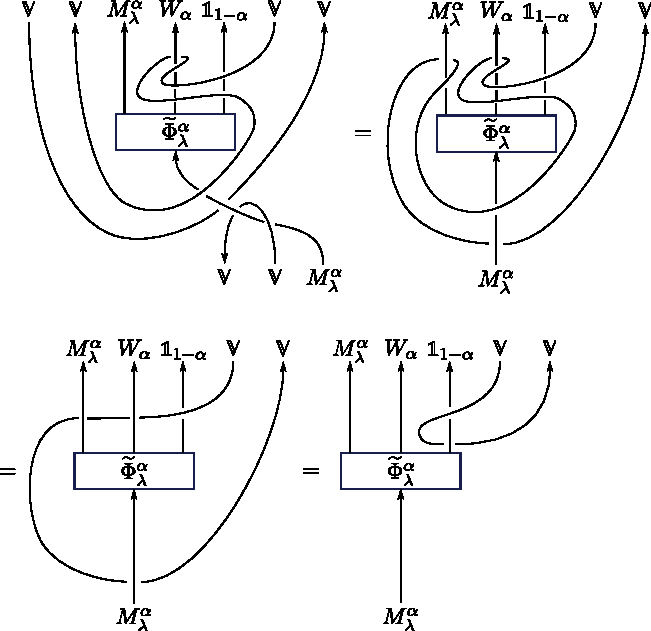
\includegraphics[scale=.8]{../assets/2518/wen_figures/tMoment.pdf}
\]
For the first equality, we~applied the modified coend relation \eqref{tHomLinRel}.
From \eqref{RFactor}, one can see that the final diagram is equal to the action of the diagram for $q^2t^{-2}\mathrm{ev}_{\mathbb{V}}$, which yields the entries of $q^2t^{-2}I$ upon contraction.
\end{proof}

We define
\begin{equation*}
\AAA_\alpha^{[t]}:=(\MM_{[t]}\big/\mathcal{I}_\alpha)^\UU,
\quad\AAA_\alpha:=K\otimes\AAA_\alpha.
\end{equation*}
Like in Proposition \ref{RedAlgProp}, $\AAA_\alpha^{[t]}$ and $\AAA_\alpha$ are in fact algebras.
Let us also define
\begin{align*}
\MM_{\mathrm{IV}}^{[t]}&:=\CC(q)[t^{pm 1}]\otimes \MM_{\mathrm{IV}},\\
\AAA_{\alpha,\mathrm{IV}}^{[t]}&:= \bigl(\MM_{\mathrm{IV}}^{[t]}\big/(\MM_{\mathrm{IV}}^{[t]}\cap\mathcal{I}_\alpha) \bigr)^\UU.
\end{align*}

\begin{prop}\label{AqtGen}
$\AAA_\alpha$ is generated by
\[
\bigl\{ \mathrm{qcoev}_{\wedge^r_q\mathbb{V}}(1), \partial_{\triangleright}\mathrm{qcoev}_{\wedge_q^r\mathbb{V}^*}(1) \bigr\}_{r=1}^n\cup
\bigl\{ \textstyle \det_q(A)^{-1}, \textstyle \det_q(B) \bigr\}.
\]
\end{prop}

\begin{proof}
Because tensoring is right exact, there is a surjective map
\[
\AAA_{k,\mathrm{IV}}\to \bigl[ \CC(q)[t^{\pm 1}]\big/ (t-q^k) \bigr]\otimes\AAA_{\alpha,\mathrm{IV}}^{[t]}.
\]
For $k>n$, the analogous generation statement for $\AAA_k$ is true due to Theorem \ref{qkCaseThm} and Lemma \ref{GenLem}.
The result follows from applying Nakayama's Lemma to each (finitely generated) bigraded piece and then localizing.
\end{proof}

\begin{lem}
The actions of $\AAA_\alpha^{[t]}$ and $\AAA_\alpha$ on $\mathrm{Int}_\alpha$ preserve the subspace $\mathrm{Int}_\alpha^+$.
\end{lem}

\begin{proof}
It suffices to prove the statement for $\AAA_\alpha$. We~then consider each of the generators given in Proposition \ref{AqtGen}.
The elements $\partial_\triangleright\mathrm{qcoev}_{\wedge_q^r\mathbb{V}^*}(1)$ and $\det_q(B)$ act by inserting central elements of $\UU$ into $\widetilde{\Phi}_\lambda^\alpha$, and thus they act diagonally.
For $\mathrm{qcoev}_{\wedge^r_q\mathbb{V}}(1)$ and $\det_q(A)^{-1}$, note that the action of either on $\widetilde{\Phi}_\lambda^\alpha$ yields the intertwiner
\[
\mathrm{id}_V\otimes\widetilde{\Phi}_\lambda^\alpha: V\otimes M_\lambda^\alpha\to V\otimes M_\lambda^\alpha\otimes W_\alpha^0
\]
for some finite-dimensional $\UU$-module $V$.
By \cite[Lem.\,5]{BGGHWt}, $V\otimes M_\lambda^\alpha$ decomposes into a direct sum of $\{M_\mu^\alpha\}$ for finitely many $\mu\in P$, and thus
\[
\mathrm{id}_V\otimes\widetilde{\Phi}_\lambda^\alpha=\sum_{\mu}c_{\lambda\mu}(q,t)\widetilde{\Phi}_\mu^\alpha
\]
for some $\{c_{\lambda\mu}(q,t)\}\subset K$. We~will show that we can set $c_{\lambda\mu}(q,t)=0$ for any $\mu\not\in P^+$ and for $\mu\in P^+$, $c_{\lambda\mu}(q,t)$ is a Pieri coefficient \cite[VI.6]{MacBook}.

To do so, let us review some details from the proof of Theorem 2 of \cite{EtKirQuant}.
Let $\rU_q(\mathfrak{n}_-)\subset\UU$ be the subalgebra generated by the $\{F_i\}$ and let $\{\beta_a\}$ be a weight basis of $\rU_q(\mathfrak{n}_-)$.
Picking a highest weight vector $v_\nu^\alpha$ for $M_\nu^\alpha$, we~obtain a weight basis $\{\beta_a v_\nu^\alpha\}$ for $M_\nu^\alpha$. We~will also make use of the natural monomial basis $\{m_c\}$ of $W_\alpha^0$, which is also a weight basis.
An intertwiner is determined by the coefficients $\{ {}_\nu\widetilde{R}_{bc}^a(q,t)\}\subset K$ such that:
\[
\widetilde{\Phi}_\nu^\alpha(\beta_a v_\nu^\alpha)=\sum_{b,c}{}_\nu\widetilde{R}_{bc}^a(q,t)\beta_b v_\nu^\alpha\otimes m_c.
\]
Given $k>0$ and $\nu\in P^+$, the subset of $\{\beta_a\}$ such that
\[
\nu-\mathrm{wt}(\beta_a)=\sum_{i}n_i\epsilon_i
\]
with $0\le n_i\le k$ likewise provides a basis for the finite-dimensional module $V_\nu^k$.
Likewise, an appropriate subset of the monomials $\{m_c\}$ give a basis of $\rU_k$.
The intertwiner~$\Phi_\nu^k$ is determined by the coefficients $\{ {}_\nu^kR_{bc}^a(q)\}\subset\CC(q)$:
\[
\Phi_\nu^k(\beta_a v_\nu^k)=\sum_{b,c}{}_\nu^k R_{bc}^a(q)\beta_b v_\nu^k\otimes m_c.
\]
In loc.\,cit., the authors showed that given $(\nu, a, b, c)$, we~have
\[
{}_\nu\widetilde{R}_{bc}^a(q,q^k)= {}_\nu^kR_{bc}^a(q)
\]
for all $k$ sufficiently large for the right-hand-side to make sense.

Now, let $v\in V$ be a weight vector and consider $v\otimes\beta_{a_\lambda}v_\lambda^\alpha$. We~can write this tensor~as
\[
v\otimes\beta_{a_\lambda}v_\lambda^\alpha = \sum_{\mu}\sum_{\ell}d_{a_\mu^\ell}(q,t)\beta_{a_\mu^\ell}v_\mu^\alpha
\]
for some coefficients $\{d_{a_\mu^\ell}(q,t)\}\subset K$.
Consider any $k$ large enough that:
\begin{itemize}
\item ${}_\lambda\widetilde{R}_{bc}^{a_\lambda}(q,q^k)= {}_\lambda^kR_{bc}^{a_\lambda}(q)$ for the $bc$-indices appearing in $\widetilde{\Phi}_\lambda^\alpha(\beta_{a_\lambda}v_\lambda^\alpha)$;
\item for $\mu\in P^+$, ${}_\mu\widetilde{R}_{bc}^{a_\mu^\ell}(q,q^k)= {}_\mu^k R_{bc}^{a_\mu^\ell}(q)$ for the $bc$-indices appearing in the evaluations $\widetilde{\Phi}_\mu^\alpha(\beta_{a_\mu^\ell}v_\mu^\alpha)$;
\item $d_{a_\mu^\ell}(q,q^k)$ is well-defined for all $a_\mu^\ell$.
\end{itemize}
The Pieri rules for $P_\lambda(q,q^k)$ yield the equality
\[
v\otimes\widetilde{\Phi}_\lambda^\alpha(\beta_{a_\lambda}v_\lambda^\alpha)\Big|_{t\mto q^k}
=
\sum_{\mu} c_{\lambda\mu}(q,t)\sum_{a_\mu^\ell}d_{a_\mu^\ell}(q,t)\widetilde{\Phi}_\mu^\alpha(\beta_{a_\mu^\ell}v_\mu^\alpha)\Big|_{t\mto q^k}.
\]
Here, by $t\mto q^k$, we~mean specialize the coefficients of the output basis $\{\beta_b v_\mu^\alpha\otimes m_c\}$.
Since this equality holds at $t=q^k$ for infinitely many values of $k$, it also holds for general $t$.
\end{proof}

The action on $\mathrm{Int}_\alpha^+$ yields an algebra homomorphism
\[
\mathfrak{rad}_\alpha:\AAA^{[t]}_\alpha\to\mathrm{End}_K(\Lambda^\pm_n(q,t))
\]
that we also call the \textit{radial parts} map.
Through analysis similar to what was done in Section~\ref{EtKirDAHA}, the analogue of Proposition \ref{DAHAContain} and its proof holds in this case as~well:
\begin{prop}\label{tDAHAContain}
Upon base change to $K$, the image of $\mathfrak{rad}_\alpha$ contains the image of $\SHH_n(q,t)$ under $\rrr$:
\[
\mathfrak{rad}_k\left(\AAA_\alpha \right)\supset\rrr\bigl(\SHH_n(q,t) \bigr).
\]
This inclusion respects the bigradings and
\begin{equation*}
\begin{aligned}
\mathfrak{rad}_\alpha\bigl(\mathrm{qcoev}_{\wedge_q^r\mathbb{V}}(1) \bigr)&= \rrr(\ee e_r(\boldsymbol{X}_n)\ee),\\
\mathfrak{rad}_\alpha\bigl(\partial_\triangleright\mathrm{qcoev}_{\wedge_q^r\mathbb{V}^*}(1) \bigr)&= q^{r(n-1)}\rrr\bigl(\ee e_r(\boldsymbol{Y}^{-1}_n)\ee \bigr),\\
\mathfrak{rad}_\alpha\bigl(\textstyle\det_q(A)^{-1}\bigr)&= \rrr(\ee \boldsymbol{X}^{-1}_n\ee),\\
\mathfrak{rad}_\alpha\bigl(\textstyle\det_q(B)\bigr)&= q^{-n(n-1)}\rrr(\ee \boldsymbol{Y}_n\ee).
\end{aligned}
\end{equation*}
\end{prop}

\begin{thm}
Upon base change to $K$, the radial parts map is an isomorphism onto $\rrr\bigl(\SHH_n(q,t) \bigr)$.
\end{thm}

\begin{proof}
On the generators from Proposition \ref{AqtGen}, one can see that specializing $\mathfrak{rad}_\alpha$ to $t=q^k$ yields $\mathfrak{rad}_k$, and thus this is true for the entirety of $\AAA_{\alpha,\mathrm{IV}}$.
Therefore, a~torsion-free element of a bigraded piece $\AAA^{[t]}_{\alpha,\mathrm{IV}}[a,b]$ in the kernel of $\mathfrak{rad}_\alpha$ must vanish at infinitely many specializations $t=q^k$.
Since $\AAA_{\alpha,\mathrm{IV}}^{[t]}[a,b]$ is finitely generated and $\CC(q)[t^{\pm 1}]$ is a PID, this implies that the kernel is torsion and hence disappears upon base change to $K$.
\end{proof}

\appendix
\refstepcounter{section}
\section*{Appendix. Modular transformations}

Here, we~investigate the relationship between the quantum radial parts map and the $\SL_2(\ZZ)$-action on the DAHA.
The main result is that our isomorphism sends a \textit{slope subalgebra} of $\SHH_n(q,t)$ to a subalgebra of $\AAA_\alpha$ generated by quantum traces of monodromy matrices over a suitable cycle on the torus.

\subsection{$\SL_2(\ZZ)$-action on DAHA}
W begin by reviewing the $\SL_2(\ZZ)$-action on the DAHA, as presented in \cite[\S3.7]{ChereDAHA}.
Recall that $\SL_2(\ZZ)$ has a presentation with generators
\[\arraycolsep3.5pt
\sigma=
\begin{pmatrix}
0 & 1\\
-1 & 0
\end{pmatrix}
,\quad\tau=
\begin{pmatrix}
1 & 0\\
1 & 1
\end{pmatrix}
\]
and relations
\[
\sigma^4=1,\quad (\sigma\tau)^3=\sigma^2.
\]
It acts on $\HH_n(q,t)$ by $R$-algebra automorphisms given by
\begin{align*}\sigma(T_i)&=T_i, &\sigma(X_i)&=Y_i^{-1}, & \sigma(Y_i)&=T_{w_0}^{-1}X_{n-i+1}T_{w_0},\\
\tau(T_i)&=T_i, & \tau(X_1\cdots X_i)&=q^i(Y_1\cdots Y_i)(X_1\cdots X_i), & \tau(Y_i)&=Y_i,
\end{align*}
where $w_0\in\Sigma_n$ is the longest element.
Since the generators fix $\{T_i\}$, it follows that $\SL_2(\ZZ)$ acts on $\SHH_n(q,t)$.

It will be easier to work with a generating set smaller than the one we used previously in \ref{Gen}:

\begin{lem}[{\cite[Lem.\,5.2]{FFJMM}}]
$\SHH_n(q,t)$ is generated by the four elements:
\[
\bigl\{\ee e_1(\boldsymbol{X}_n)\ee,\,\ee e_1(\boldsymbol{X}_n^{-1})\ee,\,\ee e_1(\boldsymbol{Y}_n)\ee,\,\ee e_1(\boldsymbol{Y}_n^{-1})\ee \bigr\}.
\]
\end{lem}

\begin{prop}
We have:
\begin{align*}
\sigma(\ee e_1(\boldsymbol{X}_n)\ee)&=\ee e_1(\boldsymbol{Y}_n^{-1})\ee, &\sigma(\ee e_1(\boldsymbol{Y}_n)\ee)&=\ee e_1(\boldsymbol{X}_n)\ee,\\
\sigma(\ee e_1(\boldsymbol{X}_n^{-1})\ee)&=\ee e_1(\boldsymbol{Y}_n)\ee, &\sigma(\ee e_1(\boldsymbol{Y}_n^{- 1})\ee)&=\ee e_1(\boldsymbol{X}_n^{-1})\ee.
\end{align*}
\end{prop}

\subsection{Gaussian}
The following element can be defined in a suitable completion of $\HH_n(q,t)$:
\begin{equation*}
\gamma:=\frac{24t^n\log(t)^2}{n(n^2-1)\log(q)}\exp\biggl(\sum_{i=1}^n\frac{\log(Y_i)^2}{\log(q)} \biggr).
\end{equation*}
Recall from \ref{PolRep} the polynomial representation $\rrr$ of $\HH_n(q,t)$, which is faithful. We~can view $\SHH_n(q,t)$ via its image $\rrr(\SHH_n(q,t))\subset\mathrm{End}(\Lambda_n^\pm(q,t))$.
Thus, rather than go into detail about the completion, we~will just confirm that $\rrr(\gamma)$ is a well-defined operator.

\begin{prop}[\cite{DiKedqt}]\label{GaussProp}
The following hold:
\begin{enumerate}
\item The action of $\gamma$ on $\Lambda_n^\pm(q,t)$ is well-defined:
\begin{equation}
\rrr(\gamma)P_\lambda(q,t)=\prod_{i=1}^nq^{\lambda_i^2}t^{(n-2i)\lambda_i}P_\lambda(q,t).
\label{GaussEigen}
\end{equation}
\item The action of $\tau\in \SL_2(\ZZ)$ on $\SHH_n(q,t)$ is equal to $\mathrm{ad}_\gamma$.
\end{enumerate}
\end{prop}

\subsection{Fourier transform}
Lemma \ref{DGenerate} can also be adapted to the case of generic~$t$.
It implies that we can define an algebra automorphism on $\AAA_\alpha$ by defining it on $\DD$ provided that it preserves invariants as well as the image of the moment map.
The analogue of the automorphism $\sigma$ is given by Definition-Proposition 6.11 of \cite{JordanMult}:
\begin{prop}
The following defines an algebra automorphism $\mathfrak{F}$ of $\DD$:
\begin{align*}
(1\otimes \mathfrak{F})(A^{\pm 1})&= B^{\pm 1}, \\
(1\otimes\mathfrak{F})(B^{\pm 1})&=q^{\mp 2n}BA^{\mp 1}B^{-1}.
\end{align*}
\end{prop}
Observe that the moment map $\mu_\DD$ \eqref{MomentDEq} is left unchanged by $\mathfrak{F}$.
It is also clear that $\mathfrak{F}$ sends quantum trace elements to other quantum trace elements.
A corollary of Proposition \ref{QTraceProp} is that $\DD^\UU$ is generated by quantum trace elements, so this implies that $\mathfrak{F}$ preserves $\DD^\UU$.
Therefore, $\mathfrak{F}$ descends to an automorphism of $\AAA_k$.

\begin{lem}
We have the following equalities in $\DD$:
\begin{align*}
\mathfrak{F}\left(\tr_q(A^{\pm 1}) \right)&= \tr_q(B^{\pm 1}),\\
\mathfrak{F}\left(\tr_q(B^{\pm 1}) \right)&= \tr_q(A^{\mp 1}).
\end{align*}
\end{lem}

\begin{proof}
Only the identities in the second row are nontrivial.
Notice we have:
\[
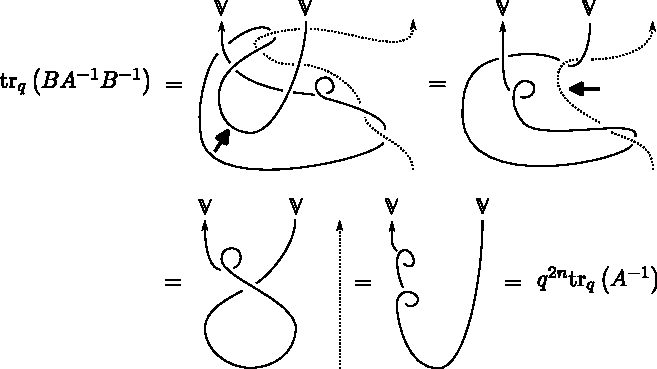
\includegraphics[scale=.8]{../assets/2518/wen_figures/fouriercalc.pdf}
\]
The constant $q^{2n}$ comes from using Proposition \ref{DrinProp} to compute $\nu^2$ on $\mathbb{V}=V_{\omega_1}$.
For $\tr_q(BAB^{-1})=q^{-2n}\tr_q(A)$, the calculations are similar.
\end{proof}

\begin{cor}\label{FourCor}
Under the isomorphism $\mathfrak{rad}_\alpha$, $\mathfrak{F}$ induces the automorphism $\sigma$ on $\rrr\bigl(\SHH_n(q,q^k)\bigr)$.
\end{cor}

\subsection{$B$-Dehn twist}
Here, we~will view the ribbon element $\nu$ as $1\otimes \nu\otimes 1\in\OO\rtimes\widetilde{\UU}^2$.
In this manner, we~can make sense of $\mathfrak{rad}_\alpha(\nu)$ by having it act on intertwiners, whereby it acts by insertion into the input.
Combining Proposition \ref{DrinProp} and Theorem \ref{EtKirMac} gives~us:
\begin{equation}
\begin{aligned}
\mathfrak{rad}_\alpha(\nu)P_\lambda(q,t)&=q^{-\langle\lambda,\lambda\rangle - \alpha\langle\lambda,2\rho\rangle -(\alpha-1)(\alpha+1)\langle\rho,\rho\rangle}P_\lambda(q,t)\\
&= q^{-(\alpha-1)(\alpha+1)\langle\rho,\rho\rangle}\prod_{i=1}^nq^{-\lambda_i^2}t^{-\lambda_i(n-2i)}P_\lambda(q,t).
\end{aligned}
\label{RibbonEigen}
\end{equation}
Comparing the $\lambda$-dependent parts of the eigenvalue with \eqref{GaussEigen} gives us:
\begin{prop}\label{GaussRibbon}
We have
\[
q^{-(\alpha-1)(\alpha+1)\langle\rho,\rho\rangle}\mathfrak{rad}_\alpha(\nu^{-1})=\rrr(\gamma).
\]
\end{prop}
From \eqref{RibbonEigen}, it is clear that conjugation by $\nu$ preserves the $\ker(\mathfrak{rad}_\alpha)$ and thus defines an algebra automorphism of $\AAA_\alpha$.
Moreover, by Propositions \ref{GaussProp} and \ref{GaussRibbon}, this action coincides with $\tau^{-1}$ on $\rrr(\SHH_n(q,t))$.
An analogue of the following lemma was proved in \cite{FaitgMod} in the setting of finite-dimensional Hopf algebras, although we note that our proof is quite different:
\begin{lem}\label{DehnD}
Conjugation by $\nu$ yields the algebra automorphism on $\DD$ induced by:
\[
(1\otimes \ad_\nu) (A)=q^n B^{-1}A,\quad
(1\otimes \ad_\nu) (B)= B.
\]
\end{lem}

\begin{proof}
Only the first equation is nontrivial. We~use \eqref{RibbonCo} to commute $\nu$ past an $A$-matrix element:
\[
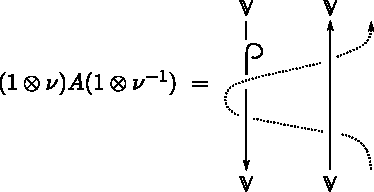
\includegraphics[scale=.8]{../assets/2518/wen_figures/Dehn1.pdf}
\]
On the other hand, we~have:
\[
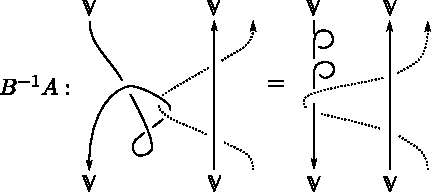
\includegraphics[scale=.8]{../assets/2518/wen_figures/DMoment1.pdf}
\]
The $q^n$ compensates for the extra loop.
\end{proof}

\subsection{Slope versus cycles}
Let
\begin{equation*}
\begin{aligned}
\SHH_n(q,t)_0&:=\bigl\langle\ee e_r(\boldsymbol{X}_n)\ee,\,\ee e_r(\boldsymbol{X}_n^{-1})\ee\bigm| 1\le r\le n\bigr\rangle,
\\
\SHH_n(q,t)_\infty&:=\bigl\langle\ee e_r(\boldsymbol{Y}_n)\ee,\, \ee e_r(\boldsymbol{Y}_n^{-1})\ee\bigm| 1\le r\le n\bigr\rangle.
\end{aligned}
\end{equation*}
For $\sfrac{b}{a}\in\QQ$ with $a$ and $b$ relatively prime, define
\[
\SHH_n(q,t)_{\sfrac{b}{a}}:=g\bigl(\SHH_n(q,t)_0\bigr)
\]
for any $g\in \SL_2(\ZZ)$ such that $g(1,0)=(a,b)$.
Such a $g$ can always be constructed using the Euclidean algorithm.
On the other hand, the definition does not depend on~$g$ since the stabilizer of $(1,0)$ is generated by
\[\arraycolsep3.5pt
\eta:=
\begin{pmatrix}
1 & -1\\
0 & 1
\end{pmatrix}
=\sigma\tau\sigma^{-1}
\]
and $\eta$ acts trivially on $\SHH_n(q,t)_0$. We~call $\SHH_n(q,t)_{\sfrac{b}{a}}$ the \textit{slope $\sfrac{b}{a}$ subalgebra}.

Analogously, we~consider the following subalgebras of $\AAA_\alpha$:
\begin{align*}
\AAA_\alpha^{(1,0)}&:=\bigl\langle\tr_q(A^m)\bigm| m\in\ZZ\bigl\rangle\cong\OO^\UU,\\
\AAA_\alpha^{(0,1)}&:=\bigl\langle\tr_q(B^m)\bigm| m\in\ZZ\bigr\rangle\cong\partial_{\triangleright}(\OO^\UU).
\end{align*}
If we view $\AAA_\alpha$ as a quantized character variety for the torus (\cf \cite{AlekScho, BBJ1, BBJ2}), then these subalgebras are generated by quantized traces of monodromy matrices over the $a$- and $b$-cycles, respectively.
Our analysis in \ref{EtKirThy} shows that:
\begin{align*}
\mathfrak{rad}_\alpha\bigl(\AAA_\alpha^{(1,0)}\bigr)&=\rrr\bigl(\SHH_n(q,t)_0\bigr),\\
\mathfrak{rad}_\alpha\bigl(\AAA_\alpha^{(0,1)}\bigr)&= \rrr\bigl(\SHH_n(q,t)_\infty\bigr).
\end{align*}
For $\sfrac{b}{a}\in\QQ$ with $a$ and $b$ relatively prime, we~define
\[
\AAA_{\alpha}^{(a,b)}:=\mathfrak{rad}_\alpha^{-1}\bigl(\rrr\bigl(\SHH_n(q,t)_{\sfrac{b}{a}} \bigr) \bigr).
\]
By Corollary \ref{FourCor} and Proposition \ref{GaussRibbon}, we~can obtain $\AAA_{\alpha}^{(a,b)}$ by applying the appropriate combinations of $\mathfrak{F}$ and $\ad_{\nu}$ to $\AAA_{\alpha}^{(1,0)}$.
Since $\sigma$ and $\tau$ generate $\SL_2(\ZZ)$, we~can make sense of the action of any $g\in \SL_2(\ZZ)$ on $\AAA_k$ in this manner.

We end with an observation relating $\sfrac{b}{a}$ and the $(a,b)$-cycle on the torus.
For a product $\Pi$ of $A$- and $B$-matrices, we~define its \textit{support}
\[
\mathrm{supp}(\Pi):=(a,b)\in\ZZ^2,
\]
where:
\begin{itemize}
\item $a$ is the sum of all exponents of $A$-matrices appearing in $\Pi$;
\item $b$ is the sum of all exponents of $B$-matrices appearing in $\Pi$.
\end{itemize}
Thus, if $\Pi$ can be viewed as a monodromy over the $(a,b)$-cycle.
The following is an easy consequence of the definition of $\mathfrak{F}$ and Lemma \ref{DehnD}:

\begin{cor}
For $g\in \SL_2(\ZZ)$, we~have
\[
g\left(\tr_q(A^m) \right)=c\tr_q(\Pi^m)
\]
for some $c\in K$ and product $\Pi$ of $A$- and $B$-matrices such that $\mathrm{supp}(\Pi)=g(1,0)$.
\end{cor}
Thus, $\AAA_\alpha^{(a,b)}$ is generated by certain quantum traces of monodromy matrices supported on the $(a,b)$-cycle.

% End literal retained input author-body.tex

\begin{thebibliography}{99}
\bibitem{AlekScho} A. Y. Alekseev \& V. Schomerus - “Representation theory of Chern-Simons observables” , Duke Math. J. 85 (1996) no. 2, p. 447-510
\bibitem{BCMN} L. Bittmann, A. Chandler, A. Mellit \& C. Novarini - “Type $A$ DAHA and doubly periodic tableaux” , Adv. Math. 416 (2023), article ID 108919, 58 pages
\bibitem{BFG} R. Bezrukavnikov, M. Finkelberg \& V. Ginzburg - “Cherednik algebras and Hilbert schemes in characteristic $p$ ” , Represent. Theory 10 (2006), p. 254-298
\bibitem{BGGHWt} I. N. Bernšteĭn, I. M. Gelʼfand \& S. I. Gelʼfand - “Structure of representations that are generated by vectors of highest weight” , Funkcional. Anal. i Priložen. 5 (1971) no. 1, p. 1-9
\bibitem{BalJor} M. Balagovic \& D. Jordan - “The Harish-Chandra isomorphism for quantum $GL_2$ ” , J. Noncommut. Geom. 12 (2018) no. 3, p. 1161-1197
\bibitem{BakKir} B. Bakalov \& A. Kirillov - Lectures on tensor categories and modular functors , University Lect. Series , vol. 21 , American Mathematical Society, Providence, RI, 2001
\bibitem{BBJ1} D. Ben-Zvi, A. Brochier \& D. Jordan - “Integrating quantum groups over surfaces” , J. Topology 11 (2018) no. 4, p. 874-917
\bibitem{BBJ2} D. Ben-Zvi, A. Brochier \& D. Jordan - “Quantum character varieties and braided module categories” , Selecta Math. (N.S.) 24 (2018) no. 5, p. 4711-4748
\bibitem{ChereAnnals} I. Cherednik - “Double affine Hecke algebras and Macdonald’s conjectures” , Ann. of Math. (2) 141 (1995) no. 1, p. 191-216
\bibitem{ChereDAHA} I. Cherednik - Double affine Hecke algebras , London Math. Soc. Lect. Note Series , vol. 319 , Cambridge University Press, Cambridge, 2005
\bibitem{DiKedqt} P. Di Francesco \& R. Kedem - “ $(t,q)$ -deformed Q-systems, DAHA and quantum toroidal algebras via generalized Macdonald operators” , Comm. Math. Phys. 369 (2019) no. 3, p. 867-928
\bibitem{DonMudRET} J. Donin \& A. Mudrov - “Reflection equation, twist, and equivariant quantization” , Israel J. Math. 136 (2003), p. 11-28
\bibitem{DrinAlmost} V. G. Drinfel’d - “Almost cocommutative Hopf algebras” , Algebra i Analiz 1 (1989) no. 2, p. 30-46
\bibitem{DrinQuasi} V. G. Drinfel’d - “Quasi-Hopf algebras” , Algebra i Analiz 1 (1989) no. 6, p. 114-148
\bibitem{EtGinz} P. Etingof \& V. Ginzburg - “Symplectic reflection algebras, Calogero-Moser space, and deformed Harish-Chandra homomorphism” , Invent. Math. 147 (2002) no. 2, p. 243-348
\bibitem{EGGO} P. Etingof, W. L. Gan, V. Ginzburg \& A. Oblomkov - “Harish-Chandra homomorphisms and symplectic reflection algebras for wreath-products” , Publ. Math. Inst. Hautes Études Sci. 105 (2007), p. 91-155
\bibitem{EtKirQuant} P. I. Etingof \& A. A. Kirillov - “Macdonald’s polynomials and representations of quantum groups” , Math. Res. Lett. 1 (1994) no. 3, p. 279-296
\bibitem{EtLatBook} P. Etingof \& F. Latour - The dynamical Yang-Baxter equation, representation theory, and quantum integrable systems , Oxford Lect. Series in Math. and its Applications , vol. 29 , Oxford University Press, Oxford, 2005
\bibitem{FaitgMod} M. Faitg - “Modular group representations in combinatorial quantization with non-semisimple Hopf algebras” , SIGMA Symmetry Integrability Geom. Methods Appl. 15 (2019), article ID 077, 39 pages
\bibitem{FFJMM} B. Feigin, E. Feigin, M. Jimbo, T. Miwa \& E. Mukhin - “Quantum continuous $\mathfrak{gl}_\infty $ : semiinfinite construction of representations” , Kyoto J. Math. 51 (2011) no. 2, p. 337-364
\bibitem{FGCurve} M. Finkelberg \& V. Ginzburg - “Cherednik algebras for algebraic curves” , in Representation theory of algebraic groups and quantum groups , Progress in Math. , vol. 284 , Birkhäuser/Springer, New York, 2010, p. 121-153
\bibitem{GanGinz} W. L. Gan \& V. Ginzburg - “Almost-commuting variety, $\mathcal{D}$ -modules, and Cherednik algebras” , Internat. Math. Res. Papers (2006), article ID 26439, 54 pages
\bibitem{GanJorSaf} I. Ganev, D. Jordan \& P. Safronov - “The quantum Frobenius for character varieties and multiplicative quiver varieties” , J. Eur. Math. Soc. (JEMS) 27 (2025) no. 7, p. 3023-3084
\bibitem{GJV} S. Gunningham, D. Jordan \& M. Vazirani - “Quantum character theory” , 2023
\bibitem{GorStaff2} I. Gordon \& J. T. Stafford - “Rational Cherednik algebras and Hilbert schemes. II. Representations and sheaves” , Duke Math. J. 132 (2006) no. 1, p. 73-135
\bibitem{GiaZhaQW} A. Giaquinto \& J. J. Zhang - “Quantum Weyl algebras” , J. Algebra 176 (1995) no. 3, p. 861-881
\bibitem{HaimPoly} M. Haiman - “Hilbert schemes, polygraphs and the Macdonald positivity conjecture” , J. Amer. Math. Soc. 14 (2001) no. 4, p. 941-1006
\bibitem{HCLie} Harish-Chandra - “On representations of Lie algebras” , Ann. of Math. (2) 50 (1949), p. 900-915
\bibitem{HCInvDiff} Harish-Chandra - “Invariant differential operators and distributions on a semisimple Lie algebra” , Amer. J. Math. 86 (1964), p. 534-564
\bibitem{HottKash} R. Hotta \& M. Kashiwara - “The invariant holonomic system on a semisimple Lie algebra” , Invent. Math. 75 (1984) no. 2, p. 327-358
\bibitem{JosLetztLocal} A. Joseph \& G. Letzter - “Local finiteness of the adjoint action for quantized enveloping algebras” , J. Algebra 153 (1992) no. 2, p. 289-318
\bibitem{JordanEll} D. Jordan - “Quantum $D$ -modules, elliptic braid groups, and double affine Hecke algebras” , Internat. Math. Res. Notices (2009) no. 11, p. 2081-2105
\bibitem{JordanMult} D. Jordan - “Quantized multiplicative quiver varieties” , Adv. Math. 250 (2014), p. 420-466
\bibitem{JorVaz} D. Jordan \& M. Vazirani - “The rectangular representation of the double affine Hecke algebra via elliptic Schur-Weyl duality” , Internat. Math. Res. Notices (2021) no. 8, p. 5968-6019
\bibitem{JorWhite} D. Jordan \& N. White - “The center of the reflection equation algebra via quantum minors” , J. Algebra 542 (2020), p. 308-342
\bibitem{KirLec} A. A. Kirillov - “Lectures on affine Hecke algebras and Macdonald’s conjectures” , Bull. Amer. Math. Soc. (N.S.) 34 (1997) no. 3, p. 251-292
\bibitem{KashRouq} M. Kashiwara \& R. Rouquier - “Microlocalization of rational Cherednik algebras” , Duke Math. J. 144 (2008) no. 3, p. 525-573
\bibitem{LevStafJams} T. Levasseur \& J. T. Stafford - “Invariant differential operators and an homomorphism of Harish-Chandra” , J. Amer. Math. Soc. 8 (1995) no. 2, p. 365-372
\bibitem{LevStafKer} T. Levasseur \& J. T. Stafford - “The kernel of an homomorphism of Harish-Chandra” , Ann. Sci. École Norm. Sup. (4) 29 (1996) no. 3, p. 385-397
\bibitem{MacBook} I. G. Macdonald - Symmetric functions and Hall polynomials , Oxford Classic Texts in the Physical Sciences , The Clarendon Press, Oxford University Press, New York, 2015
\bibitem{MajidBraided} S. Majid - “Braided groups” , J. Pure Appl. Algebra 86 (1993) no. 2, p. 187-221
\bibitem{MortSamDAHA} H. R. Morton \& P. Samuelson - “DAHAs and skein theory” , Comm. Math. Phys. 385 (2021) no. 3, p. 1655-1693
\bibitem{ObDAHA} A. Oblomkov - “Double affine Hecke algebras and Calogero-Moser spaces” , Represent. Theory 8 (2004), p. 243-266
\bibitem{ReshTurRibbon} N. Y. Reshetikhin \& V. G. Turaev - “Ribbon graphs and their invariants derived from quantum groups” , Comm. Math. Phys. 127 (1990) no. 1, p. 1-26
\bibitem{SchiffVassMac} O. Schiffmann \& E. Vasserot - “The elliptic Hall algebra, Cherednik Hecke algebras and Macdonald polynomials” , Compositio Math. 147 (2011) no. 1, p. 188-234
\bibitem{VarVassRoot} M. Varagnolo \& E. Vasserot - “Double affine Hecke algebras at roots of unity” , Represent. Theory 14 (2010), p. 510-600
\bibitem{WallachInv} N. R. Wallach - “Invariant differential operators on a reductive Lie algebra and Weyl group representations” , J. Amer. Math. Soc. 6 (1993) no. 4, p. 779-816
\bibitem{WeylInv} H. Weyl - The classical groups. Their invariants and representations , Princeton University Press, Princeton, NJ, 1939
\end{thebibliography}
\end{document}
